% =====================================================================
%  Semester thesis — X. Lu, TUM CIT, Chair of Robotics, Artificial
%  Intelligence and Real-time Systems (Prof. Knoll)
%  Layout follows the TUM CIT thesis look (Charter body, Helvetica
%  headings, TUM blue title page). Build:  latexmk -pdf main.tex
% =====================================================================
\documentclass[11pt,a4paper,oneside,chapterprefix=true,headings=big,parskip=false,numbers=noenddot,bibliography=totoc,listof=totoc]{scrreprt}

% ---------- fonts and language ----------
\usepackage[charter]{mathdesign}
\usepackage[UTF8,scheme=chinese,heading=false,fontset=none,zihao=false]{ctex}
\setmainfont{XCharter}[Extension=.otf,UprightFont=*-Roman,BoldFont=*-Bold,ItalicFont=*-Italic,BoldItalicFont=*-BoldItalic]
\setsansfont{TeX Gyre Heros}[Scale=0.92]
\setCJKmainfont{Noto Serif CJK SC}[BoldFont=Noto Serif CJK SC Bold]
\setCJKsansfont{Noto Sans CJK SC}[BoldFont=Noto Sans CJK SC Bold]
\setCJKmonofont{Noto Sans CJK SC}
\linespread{1.25}

% ---------- page geometry and headers ----------
\usepackage[a4paper,left=30mm,right=30mm,top=32mm,bottom=32mm,headsep=10mm]{geometry}
\usepackage[automark,headsepline=false]{scrlayer-scrpage}
\clearpairofpagestyles
\ihead{\sffamily\itshape\small\headmark}
\ohead{\sffamily\bfseries\small\pagemark}
\renewcommand*{\chaptermarkformat}{}
\automark[section]{chapter}
\setkomafont{pageheadfoot}{\normalfont}
\setkomafont{disposition}{\sffamily\bfseries}
\setkomafont{chapterprefix}{\huge}
\renewcommand*{\chapterformat}{第\,\thechapter\,章}
\RedeclareSectionCommand[beforeskip=40mm,afterskip=18mm,innerskip=10mm]{chapter}
\RedeclareSectionCommand[beforeskip=-4ex plus -1ex minus -.2ex,afterskip=2.2ex]{section}

% ---------- math, units, tables, figures ----------
\usepackage{amsmath}
\usepackage{bm}
\usepackage{siunitx}
\sisetup{per-mode=power,range-phrase=\,--\,,range-units=single,detect-all,list-separator={、},list-final-separator={和},list-pair-separator={和}}
\usepackage{booktabs,tabularx,multirow,array}
\usepackage{graphicx}
\graphicspath{{../figures/}}
\usepackage[font=small,labelfont={bf,sf},format=hang]{caption}
\usepackage{subcaption}
\usepackage{float}
\usepackage{xcolor}
\definecolor{TUMblue}{HTML}{0065BD}
\definecolor{todo}{HTML}{C0392B}
\usepackage{tikz}
\usetikzlibrary{arrows.meta,positioning,calc,fit,backgrounds,decorations.pathmorphing,patterns}
\usepackage{enumitem}
\setlist{itemsep=2pt,topsep=4pt}
\usepackage{csquotes}

% ---------- bibliography ----------
\usepackage[backend=biber,style=alphabetic,maxbibnames=99,maxcitenames=2,giveninits=true,doi=true,url=false,isbn=false,eprint=true]{biblatex}
\addbibresource{../refs.bib}
\AtEveryBibitem{\clearfield{note}}

% ---------- cross references ----------
\usepackage[hidelinks,pdfusetitle]{hyperref}
\usepackage[capitalise,noabbrev,nameinlink]{cleveref}
\crefformat{chapter}{第~#2#1#3~章}\Crefformat{chapter}{第~#2#1#3~章}
\crefrangeformat{chapter}{第~#3#1#4~章至第~#5#2#6~章}
\crefmultiformat{chapter}{第~#2#1#3~章}{和第~#2#1#3~章}{、第~#2#1#3~章}{和第~#2#1#3~章}
\crefformat{section}{#2#1#3~节}\Crefformat{section}{#2#1#3~节}
\crefmultiformat{section}{#2#1#3~节}{和~#2#1#3~节}{、#2#1#3~节}{和~#2#1#3~节}
\crefrangeformat{section}{#3#1#4~节至~#5#2#6~节}\Crefrangeformat{section}{#3#1#4~节至~#5#2#6~节}
\crefrangeformat{figure}{图~#3#1#4~至~#5#2#6}\crefrangeformat{table}{表~#3#1#4~至~#5#2#6}
\crefmultiformat{subsection}{#2#1#3~节}{和~#2#1#3~节}{、#2#1#3~节}{和~#2#1#3~节}
\crefformat{appendix}{附录~#2#1#3}\crefmultiformat{appendix}{附录~#2#1#3}{和附录~#2#1#3}{、附录~#2#1#3}{和附录~#2#1#3}
\crefformat{subsection}{#2#1#3~节}\Crefformat{subsection}{#2#1#3~节}
\crefformat{figure}{图~#2#1#3}\Crefformat{figure}{图~#2#1#3}
\crefmultiformat{figure}{图~#2#1#3}{和~#2#1#3}{、#2#1#3}{和~#2#1#3}
\crefformat{table}{表~#2#1#3}\Crefformat{table}{表~#2#1#3}
\crefmultiformat{table}{表~#2#1#3}{和~#2#1#3}{、#2#1#3}{和~#2#1#3}
\crefformat{equation}{式~(#2#1#3)}\Crefformat{equation}{式~(#2#1#3)}
\crefrangeformat{equation}{式~(#3#1#4)~至~(#5#2#6)}
\crefformat{appendix}{附录~#2#1#3}\Crefformat{appendix}{附录~#2#1#3}

% ---------- helpers ----------
\setlength{\emergencystretch}{3em}
\newcommand{\TODO}[1]{\textcolor{todo}{\textbf{[TODO:} #1\textbf{]}}}
\newcommand{\U}{U}                          % swimming / tow speed
\newcommand{\Tm}{\bar{T}}                   % cycle-mean thrust
\newcommand{\Pm}{\bar{P}}                   % cycle-mean input power
\newcommand{\etaF}{\eta}                    % Froude efficiency
\newcommand{\mNs}{\si{\milli\newton}}
\newcommand{\ms}{\si{\metre\per\second}}
\newcommand{\sfit}[1]{\textsf{#1}}

% ---------- title data ----------
\newcommand{\thesistype}{Semester Thesis in Mechatronics, Robotics, and Biomechanical Engineering（中文译本）}
\newcommand{\thesistitle}{Hydrodynamic Modeling and Trajectory Optimization of Paddling Propulsion for a Quadruped Robot}
\newcommand{\thesistitlezh}{四足机器人划水推进的水动力建模与轨迹优化}
\newcommand{\thesisauthor}{Xiaotian Lu}
\newcommand{\thesissupervisor}{Prof.\ Dr.-Ing.\ habil.\ Alois C.\ Knoll}
\newcommand{\thesisadvisor}{Qian Huang, M.Sc.}
\newcommand{\thesisdate}{2026 年 10 月}      % TODO: 提交日期
\hypersetup{pdftitle={\thesistitle},pdfauthor={\thesisauthor}}

\begin{document}
\renewcommand{\contentsname}{目录}
\renewcommand{\listfigurename}{插图目录}
\renewcommand{\listtablename}{表格目录}
\renewcommand{\figurename}{图}
\renewcommand{\tablename}{表}
\renewcommand{\appendixname}{附录}
\pagenumbering{roman}
% ---------------- 封面（TUM CIT 样式，中文译本） ----------------
\begin{titlepage}
\newgeometry{left=25mm,right=25mm,top=20mm,bottom=25mm}
\sffamily
\begin{minipage}[t]{0.7\textwidth}
  {\color{TUMblue}\small TUM School of Computation, Information and Technology\\
  Technical University of Munich}
\end{minipage}\hfill
\begin{minipage}[t]{0.25\textwidth}\raggedleft
  \IfFileExists{../figures/tum_logo.pdf}{
\includegraphics[height=10.5mm]{tum_logo}}{\color{TUMblue}\fbox{\parbox[c][10mm][c]{24mm}{\centering\tiny TUM logo\\(from template)}}}
\end{minipage}

\vspace*{65mm}
{\large \thesistype\par}
\vspace{8mm}
{\noindent\raggedright\color{TUMblue}\bfseries\fontsize{24}{32}\selectfont \thesistitlezh\par}
\vspace{5mm}
{\noindent\raggedright\hyphenpenalty=10000\color{TUMblue}\fontsize{15}{19}\selectfont \thesistitle\par}
\vfill
\begin{tabular}{@{}p{45mm}l}
\textbf{导师（Supervisor）} & \thesissupervisor\\[3mm]
\textbf{指导（Advisor）}    & \thesisadvisor\\[3mm]
\textbf{作者（Author）}     & \thesisauthor\\[3mm]
\textbf{日期（Date）}       & \thesisdate，慕尼黑
\end{tabular}
\restoregeometry
\end{titlepage}

\thispagestyle{empty}
\vspace*{40mm}
\noindent{\sffamily\bfseries\LARGE 声明\par}
\vspace{14mm}
\noindent 本人确认，本学期论文为本人独立完成，所使用的全部资料与来源均已注明。在撰写过程中，作者使用 Claude（Anthropic）
辅助编写数据后处理脚本、生成图表及润色语言。所有由 AI 辅助生成的文字和代码均经作者审阅、修改和核实。全部技术思路、仿真设置、
分析、结果、图表内容与结论均由作者完成并核实。

\vspace{6mm}
\noindent 本文为英文原稿的中文译本；如有出入，以英文原稿为准。

\vspace{25mm}
\noindent 慕尼黑，\thesisdate\hfill\begin{tabular}[t]{c}\rule{60mm}{0.4pt}\\ \footnotesize(\thesisauthor)\end{tabular}
\cleardoublepage

\thispagestyle{empty}
\vspace*{25mm}
\noindent{\sffamily\bfseries\Large 摘要\par}
\vspace{6mm}
\noindent
两栖四足机器人可以通过摆动腿部来游泳，但为行走而设计的腿并不是好的推进器。本文研究哪种推进原理适合四足机器人BODY2的腿，以及每种推进器应如何运动。本文将采用折扇桨的阻力型划水与装在同一条腿上的小型尾鳍的升力型拍动进行比较。研究采用了三种作用各不相同的仿真工具。首先，将一个含有作用于各连杆的Morison型力和执行器速度限制的MuJoCo降阶模型与CMA-ES步态优化相结合。只要模型中包含升力且升力未被抑制，所有可行的优化步态都是升力推进的，且在相同航速下，升力步态所需功率仅为纯阻力模型中最佳步态的二分之一到三分之一。其次，在OpenFOAM中采用重叠网格CFD对单腿进行仿真。对于折扇桨，采用梯形速度规律、12\,mm的收拢宽度并在减速开始时合扇，可使静止状态下每条腿的推力从机器人当前步态的\SI{23.4}{\milli\newton}提高到\SIrange{73}{83}{\milli\newton}；该范围涵盖了折叠时附加质量的变化，而折扇的两态模型并不解析这一变化。桨的推力在航速约\SI{0.30}{\metre\per\second}时消失，因为其回程阻力以及在迎面来流中开扇的代价不断增大，而划水冲程推力则逐渐衰减。尾鳍在静止时产生相同的单位面积推力，且其推力随航速下降得更慢。二者的推力和效率分别在约\SI{0.24}{}和\SI{0.22}{\metre\per\second}处出现交叉。使尾鳍俯仰角随航速调度，可将攻角保持在\SI{20}{\degree}附近，并使\SI{0.30}{\metre\per\second}时的弗劳德效率从0.24提高到0.40。准定常自航平衡预测尾鳍的巡航速度为\SI{0.30}{\metre\per\second}，优化后的桨为\SIrange{0.26}{0.27}{\metre\per\second}，且采用随航速调度俯仰的尾鳍所需功率低43\,\%。装配尾鳍的机器人在\SI{2}{\hertz}下的首次硬件测试比预测慢1.3至1.6倍，因此这些速度是现有机器人的上限。第三，实时求解器Flare Live提供尾鳍的参考运动，但其格子未能解析翼型、低估了尾鳍推力，因此仅用于趋势分析。所用CFD设置对一项拍动翼实验推力系数的复现误差在8\,\%以内。

\vspace{12mm}
\noindent{\sffamily\bfseries\Large Abstract\par}
\vspace{6mm}
\noindent
Amphibious quadruped robots can swim by moving their legs, but a leg designed for walking makes a poor
propulsor. This thesis asks which propulsion principle suits the legs of the quadruped BODY2 and how each
propulsor should move. Drag-based paddling with a folding fan paddle is compared with lift-based flapping of a
small fluke fitted to the same leg. Three simulation tools with different roles are used. First, a reduced-order
MuJoCo model with Morison-type link forces and an actuator speed limit is combined with CMA-ES gait
optimization. Whenever the model contains lift and lift is not suppressed, every feasible optimized gait is lift-propelled, and at equal speed the lift gaits
need one half to one third of the power of the best gaits of a drag-only model. Second, the single leg is simulated
with overset-grid CFD in OpenFOAM. For the fan paddle, a trapezoidal velocity law, a 12-mm folded width and
closing the fan at the start of the deceleration raise the thrust from \SI{23.4}{\milli\newton} for the robot's
current gait to \SIrange{73}{83}{\milli\newton} per leg at rest; the range bounds the change of added mass at the
fold, which the two-state model of the folding fan does not resolve. The paddle loses its thrust by about
\SI{0.30}{\metre\per\second}, because its recovery drag and the cost of opening the fan in the oncoming flow grow
while its power-stroke thrust decays. The fluke produces the same thrust per area at rest and loses it more slowly with speed.
Thrust and efficiency cross over at about \SI{0.24}{} and \SI{0.22}{\metre\per\second}. Scheduling the fluke pitch with speed keeps the angle of attack near
\SI{20}{\degree} and raises the Froude efficiency at \SI{0.30}{\metre\per\second} from 0.24 to 0.40. A
quasi-steady self-propulsion balance predicts a cruising speed of \SI{0.30}{\metre\per\second} for the fluke and
\SIrange{0.26}{0.27}{\metre\per\second} for the optimized paddle, with 43\,\% less power for the fluke with
speed-scheduled pitch. A first hardware test with flukes at \SI{2}{\hertz} is 1.3 to 1.6 times slower than predicted, so these
speeds are upper bounds for the present robot. Third, the real-time solver Flare Live supplies the reference fluke motion, but its lattice does not resolve the
foil and it underpredicts the fluke thrust, so it is used for trends only. The CFD set-up
reproduces the thrust coefficient of a flapping-foil experiment to within 8\,\%.
\cleardoublepage

\pagestyle{scrheadings}
\tableofcontents
\listoffigures
\listoftables
\chapter*{缩略语与符号}
\addcontentsline{toc}{chapter}{缩略语与符号}
\markboth{缩略语与符号}{缩略语与符号}

\begin{description}[labelwidth=16mm,leftmargin=20mm,itemsep=1pt,font=\normalfont\bfseries]
\item[AR] 展弦比（aspect ratio），$\mathit{AR}=b^2/S$
\item[BL] 体长（body length），速度以BL/s计
\item[CFD] 计算流体力学（computational fluid dynamics）
\item[CMA-ES] 协方差矩阵自适应进化策略（covariance matrix adaptation evolution strategy）
\item[COT] 运输代价（cost of transport）
\item[EMF] 电动势（electromotive force），即舵机电机的反电动势
\item[GCI] 网格收敛指数（grid convergence index）
\item[LSTM] 长短期记忆（long short-term memory），一种循环神经网络
\item[MJCF] MuJoCo的XML模型格式（MuJoCo XML model format）
\item[PIMPLE] PISO与SIMPLE合并的压力--速度耦合算法（merged PISO--SIMPLE pressure--velocity coupling algorithm）
\item[RMS] 均方根（root mean square）
\item[SPH] 光滑粒子流体动力学（smoothed-particle hydrodynamics）
\item[URDF] 统一机器人描述格式（unified robot description format）
\end{description}

\bigskip
\begin{description}[labelwidth=16mm,leftmargin=20mm,itemsep=1pt,font=\normalfont]
\item[$\U$] 前进速度（游动速度或拖曳速度），\si{\metre\per\second}
\item[$f,\;T$] 冲程频率与周期，$T=1/f$
\item[$\tau$] 周期相位$t/T\bmod 1$
\item[$\Tm$] 单腿的周期平均推力，\si{\milli\newton}
\item[$\Pm$] 单腿的周期平均水动力输入功率，\si{\milli\watt}
\item[$\etaF$] 弗劳德效率$\Tm\U/\Pm$
\item[$C_T$] 推力系数$\Tm/(\tfrac12\rho\U^2S)$
\item[$\mathit{St}$] 斯特劳哈尔数$fA/\U$，其中$A$为峰峰值摆幅
\item[$\alpha$] 攻角，即翼型弦线与相对来流之间的夹角
\item[$\gamma$] 沉浮翼型的来流角，$\gamma=\arctan(\dot h/\U)$
\item[$\theta$] 尾鳍俯仰角
\item[$\mathrm{DUTY}$] 占空比，即划水冲程占整个周期的比例
\item[$\tau_o,\tau_c$] 折扇桨开扇和合扇时的相位
\item[$K$] $D=K\U|\U|$中的船体阻力系数，\si{\newton\second\squared\per\metre\squared}
\item[$\rho,\nu$] 水的密度与运动黏度
\end{description}

\bigskip
\noindent\textbf{算例名称}
\begin{description}[labelwidth=16mm,leftmargin=20mm,itemsep=1pt,font=\normalfont\bfseries]
\item[机器人步态] 折扇桨，采用机器人当前的冲程（周期\SI{1.25}{\second}，折叠至\SI{30}{\milli\metre}）
\item[V1--V3] 静止时阻力型冲程的各设计步骤；V3trap：优化后的冲程（梯形速度规律，折叠至\SI{12}{\milli\metre}，提前合扇）
\item[L0] 尾鳍，采用来自Flare Live的参考运动，航速\SI{0.223}{\metre\per\second}；L0c：同一算例在粗网格上的结果
\item[L2] L0运动在其他航速下的算例（\SIlist{0;0.08;0.15;0.30}{\metre\per\second}）
\item[L1] 尾鳍，采用攻角规律（L1a10、L1a28：目标攻角为\SI{10}{}和\SI{28}{\degree}）
\item[L3] 尾鳍，采用随航速调度的俯仰$\theta_0=\gamma_\text{max}/2$（L3U030、L3U040：航速\SI{0.30}{}和\SI{0.40}{\metre\per\second}）
\item[确认] 按Schouveiler等人设置的沉浮加俯仰NACA\,0012翼型算例（\cref{sec:ver-v1}）
\end{description}


\cleardoublepage
\pagenumbering{arabic}
\chapter{引言}
\label{ch:intro}

\section{研究动机}

腿式机器人在陆地上运动灵活，而它们能够发挥作用的许多场所，如海岸线、洪涝区、池塘和河岸，也都存在开阔水域。四足机器人要穿越这类水域，就需要在足部不再接触地面时有某种自我推进的方式。加装推力器（thruster）是一种选择\cite{Yao2023}，但推力器会增加质量、体积和执行器，而这些在陆地上毫无用处。另一种方案是直接用腿本身游泳\cite{Li2019,Qu2025,Han2025,Wang2025}。这样便无需额外硬件，游泳问题就转化为如何驱动现有关节以及足部应采用何种形状的问题。

用腿游泳的动物采用两种不同的物理原理\cite{Fish1996}。狗、麝鼠或鸭子以\emph{划水}（paddling）方式游泳。它们用垂直于运动方向的足向后推水，然后再将足收回到前方\cite{Fish1984,Fish2021DogPaddle}。推力来自划水冲程（power stroke）中足所受的阻力，而回程（recovery stroke）不可避免地会损失一部分推力。海豚、海龟和许多鱼类则横向于游动方向\emph{拍动}（flapping）鳍或尾鳍（fluke）。鳍以较小的攻角（angle of attack）迎向来流并产生升力，升力的前向分量即为推力。阻力型划水（drag-based paddling）结构简单，在静止时即可工作，且加速性能好。升力型拍动（lift-based flapping）在巡航速度（cruising speed）下的效率是前者的两到三倍\cite{Fish1996,Walker2000}。完全转为水生的哺乳动物都从第一种原理过渡到了第二种原理。

大多数游泳腿式机器人采用第一种原理，因为行走用的足本身就是一支桨（paddle）。本文研究这一选择对于小型两栖四足机器人BODY2是否合适，以及在每种原理下腿应如何运动。该机器人的腿是为行走而设计的。每条腿都是由两个航模舵机（servo）驱动的平面两自由度连杆机构（linkage），足部是一支在回程中折叠的扇形桨。其当前的游泳步态（gait）取自机器人的视频，并非针对推力而设计。这支桨能否做到高效，抑或在同一条腿上装一个产生升力的小型尾鳍会更好，仅凭文献无法判断，因为答案取决于腿部几何、执行器限值和游动速度。

\section{问题描述与研究范围}

本文要解决的问题是：对于给定的腿和给定的执行器，找出能最有效地推进机器人的推进器（propulsor）及周期性腿部运动，并量化该答案如何随游动速度变化。以下三个特性使这一问题颇具难度。

第一，流动是非定常且分离的。桨在每个周期内起停两次，每次停止时都会脱落一个涡，并会与自身的尾流相遇。拍动的尾鳍工作在$10^3$--$10^4$的雷诺数范围内，此时前缘涡（leading-edge vortex）以及沉浮（heave）与俯仰（pitch）之间的相位差决定了推力\cite{Triantafyllou1991,Anderson1998}。准定常（quasi-steady）模型能够捕捉这些效应的趋势，但无法给出其量级\cite{Kim2011}。

第二，答案取决于航速。静止时，桨推动的是不动的水，并在划水冲程的大部分时间内产生推力。有航速时，迎面来流会减小划水冲程中的相对速度，并增大回程中的相对速度。升力型翼型（foil）的表现则相反：其攻角由沉浮速度与游动速度之比决定，因此它通过运动学与航速相关。所以，仅在单一航速下进行比较，可能得出偏向任一原理的结论。

第三，没有哪一个模型能同时做到准确且计算代价低。单腿的三维CFD仿真需要数小时到数天，无法嵌入需要数千次评估的优化器中。降阶模型（reduced-order model）可以做到这一点，但其系数未经标定，其升力模型也只是教科书式的平板模型。

因此，本文使用三种仿真工具，各自回答不同的问题，且不要求任何一种工具复现其他工具的数值：
\begin{itemize}
  \item 在MuJoCo中建立的\emph{降阶}整机模型，结合CMA-ES步态优化，回答\emph{机理}问题：在执行器和稳定性约束下，优化器会选择哪种推进原理？其系数未经标定，因此仅用于判断方向，而不用于给出量级；
  \item 在OpenFOAM中采用重叠网格（overset grid）对真实BODY2腿部几何进行的\emph{单腿CFD}，回答\emph{量级}问题：每种推进器在不同前进速度下产生多大的推力和功率，以及一种推进器在何处反超另一种。它已通过一项实验予以确认，并提供了本文的全部定量结果；
  \item \emph{整机}实时求解器Flare Live提供参考尾鳍运动。其尾鳍推力经与CFD对比校核后发现偏低，因此其结果仅用于趋势分析。
\end{itemize}
\Cref{fig:overview}展示了这三种工具及其结果之间的联系。当降阶模型与CFD的结果不一致时，以CFD为准；这种不一致本身将在\cref{sec:disc-models}中分析。

\begin{figure}[t]
  \centering
  \begin{tikzpicture}[>=Latex,font=\small,
      box/.style={draw=TUMblue,thick,rounded corners=2pt,align=center,inner sep=4pt,text width=35mm,minimum height=17mm,fill=TUMblue!6,execute at begin node={\hyphenpenalty=10000\relax}},
      res/.style={draw=black!45,rounded corners=2pt,align=center,inner sep=3pt,text width=35mm,minimum height=9mm,fill=black!3,font=\footnotesize,execute at begin node={\hyphenpenalty=10000\relax}},
      lab/.style={font=\footnotesize\itshape,text=black!60}]
    \node[box,font=\small] (mj) at (0,0) {\textbf{降阶模型}\\MuJoCo，Morison力，\\舵机模型，\\CMA-ES（\cref{ch:mujoco}）};
    \node[box] (cfd) at (5.1,0) {\textbf{单腿CFD}\\OpenFOAM，重叠网格，\\真实腿部几何\\（\cref{ch:cfd,ch:verification}）};
    \node[box] (fl) at (10.2,0) {\textbf{整机模型}\\Flare Live，格子\\玻尔兹曼，实时\\（\cref{sec:cfd-flare}）};
    \node[lab,above=1pt of mj.north] {快速，未标定};
    \node[lab,above=1pt of cfd.north] {解析流场，已确认};
    \node[lab,above=1pt of fl.north] {整机，分辨率粗};
    \node[res] (r1) at (0,-2.3) {机理：优化器\\选择哪种原理（RQ1）};
    \node[res] (r2) at (5.1,-2.3) {推力、功率、效率\\随航速的变化；交叉点（RQ2）};
    \node[res] (r3) at (10.2,-2.3) {尾鳍推力的交叉校核（\cref{sec:ver-flare}）};
    \node[res] (sp) at (5.1,-4.2) {自航估计$4\bar T(U)=D(U)$（RQ3）};
    \node[res] (hw) at (10.2,-4.2) {首次硬件测试\\（\cref{sec:res-hw}）};
    \draw[->] (mj) -- (r1); \draw[->] (cfd) -- (r2); \draw[->] (fl) -- (r3); \draw[->] (r2) -- (sp);
    \draw[->,dashed] (mj.east) -- node[above,lab,fill=white,inner sep=1pt]{升力？} (cfd.west);
    \draw[->,dashed] (fl.west) -- node[above,lab,fill=white,inner sep=1pt]{L0运动} (cfd.east);
    \draw[->,dashed] (r2.east) -- node[above,lab,fill=white,inner sep=1pt]{尾鳍推力} (r3.west);
    \draw[<->,dashed] (sp.east) -- node[above,lab,fill=white,inner sep=1pt]{对比} (hw.west);
  \end{tikzpicture}
  \caption[方法概览]{三种仿真工具及其作用的概览。实线箭头：结果；虚线箭头：工具之间传递的信息。降阶模型促成了升力型推进器的引入，Flare Live提供参考尾鳍运动，CFD则为自航估计提供推力曲线，并作为校核Flare Live尾鳍推力的参考。}
  \label{fig:overview}
\end{figure}

研究范围限定如下。
\begin{itemize}
  \item \emph{环境。}机器人在静水水面游动。不考虑波浪、水流以及水陆之间的过渡。所有推进器CFD均为带刚性盖（rigid lid）的单相计算；未对自由液面（free surface）建模。
  \item \emph{运动。}仅考虑稳态、周期性的直线前进游动。不考虑转向、起步和反馈控制。
  \item \emph{推进器。}比较装在同一条腿上的两种推进器：机器人的折扇桨（folding fan paddle，阻力型）和装在销轴关节上的小型后掠尾鳍（swept fluke，升力型）。仿真中尾鳍俯仰角为给定值；硬件上采用的销轴加弹簧的被动实现方式未进行仿真。
  \item \emph{评价。}推力和水动力输入功率（hydrodynamic input power）仅针对推进器本身（折扇或尾鳍）计算，不含连杆。游动速度由准定常力平衡预测，并考虑一定范围的船体阻力（hull resistance）。硬件实验仅限于一次从静止起步的初步计时测试。
\end{itemize}

\section{研究问题与假设}

本文的核心问题是：
\begin{quote}
\itshape 阻力型划水与升力型拍动，哪一种推进原理能让BODY2的腿游得更快、更高效？每种推进器又应如何运动？
\end{quote}
该问题被分解为三个研究问题（research question），每个研究问题对应一个假设（hypothesis）。

\begin{description}[leftmargin=12mm,style=nextline]
\item[(RQ1)] \emph{降阶优化。}在执行器速度限值和姿态限值下，于降阶水动力模型中优化整机步态时，优化器会选择哪种推进机理？该答案是否取决于模型中所包含的物理效应？

  \emph{假设H1。}若模型包含升力项，优化器会采用升力型冲程，且在相同航速下，这些冲程所需功率低于阻力型冲程。

\item[(RQ2)] \emph{不同航速下的阻力与升力。}对于真实的腿部几何，在从静止到\SI{0.4}{\metre\per\second}的范围内，经过优化的阻力型桨和升力型尾鳍的推力、功率和弗劳德效率（Froude efficiency）各有多大？各推进器又受什么因素限制？

  \emph{假设H2。}优化后的桨在低速时推力更大，但由于回程所遭遇的迎面来流不断增强，其推力随航速急剧下降。尾鳍在静止时推力较小，但在有航速时能保留更大比例的推力，并在航速超过某一交叉点（crossover）后推力更大、效率也更高。当尾鳍的俯仰角随航速调整、使攻角保持在拍动翼的高效区间（约\SIrange{15}{25}{\degree}）附近时，尾鳍性能最佳。

\item[(RQ3)] \emph{整机。}由此可得整机的巡航速度和功率是多少？

  \emph{假设H3。}两种优化后的推进器达到相近的巡航速度，该速度由船体和连杆的阻力决定，但尾鳍所需功率更低。
\end{description}

\cref{ch:mujoco}回答RQ1。在\cref{ch:cfd,ch:verification}介绍CFD方法及其验证之后，\cref{ch:results}回答RQ2和RQ3。\Cref{ch:discussion}对各假设进行评价。

\section{贡献}

本文的贡献（contribution）如下：
\begin{enumerate}
  \item \emph{带执行器模型的降阶步态优化流程}（\cref{ch:mujoco}）。
        将带有可选平板升力项的Morison型连杆力、舵机的直流电机转矩--转速模型以及可行性优先（feasibility-first）约束与CMA-ES相结合。在模型含升力且不限制升力占比时得到的全部101个可行最优解中，均由升力提供前向冲量，而阻力与之相抗。借助升力占比限值，可以在同一模型内比较阻力型与升力型划动。
  \item \emph{针对BODY2折扇桨的优化阻力型冲程}（\cref{sec:res-drag}）。对真实腿部进行重叠网格CFD，并以两态合成（two-state composite）描述折扇，得到一种采用梯形速度规律、12\,mm收拢宽度（folded width）和提前合扇的冲程，其在静止时每条腿产生\SIrange{73}{83}{\milli\newton}的推力，是机器人当前步态的3.1--3.5倍。两态合成无法解析的附加质量（added mass）变化，则借助由CFD辨识出的附加质量进行解析界定。
  \item \emph{同一条腿上阻力型与升力型推进器随航速变化的对比}
        （\cref{sec:res-compare}）。计算了从静止到\SI{0.40}{\metre\per\second}范围内的推力、功率和效率。阻力型桨的速度上限被追溯到其回程；推力和效率的交叉点分别位于约\SI{0.24}{}和\SI{0.22}{\metre\per\second}处；随航速调度的尾鳍俯仰（speed-scheduled pitch）使尾鳍在\SI{0.30}{\metre\per\second}时的效率从0.24提高到0.40。
  \item \emph{自航（self-propulsion）估计与保真度评估}（\cref{sec:res-selfprop,ch:verification}）。
        利用一定范围的船体阻力给出巡航速度的界限；以一项拍动翼实验对CFD设置进行确认（validation），并检查了网格收敛与周期收敛（cycle convergence）；同时在相同的尾鳍运动下量化了实时求解器Flare Live的推力不足。
\end{enumerate}

\section{论文结构}

\Cref{ch:related}综述动物和机器人中的阻力型与升力型游泳、拍动翼水动力学以及游泳腿式机器人的仿真方法。\Cref{ch:foundations}介绍全文所用的物理量和简化模型：准定常划水、拍动翼运动学以及自航平衡。\Cref{ch:platform}描述机器人、两种推进器及其腿部运动。
\Cref{ch:mujoco}介绍降阶模型和步态优化。\Cref{ch:cfd}描述单腿CFD和整机Flare Live模型，\cref{ch:verification}对CFD进行验证（verification）与确认，并以其为基准校核实时求解器。
\Cref{ch:results}报告阻力型冲程的设计、升力型尾鳍、二者的比较、尾鳍俯仰角的航速调度规律以及自航估计。
\Cref{ch:discussion}解读结果并说明局限性，\cref{ch:conclusion}总结全文并展望未来工作。附录汇集了补充数据、降阶模型的肢间协调结果（\cref{app:coord}）、Flare Live结果（\cref{app:flare-trends}）以及复现本工作所需的信息。

\chapter{相关工作}
\label{ch:related}

本章综述以下内容：关于动物和翼型的阻力型（drag-based）与升力型（lift-based）游泳的已有认识，游泳腿式机器人是如何设计和仿真的，以及本文所针对的研究空白。

\section{动物的阻力型与升力型游泳}
\label{sec:rw-bio}

Fish \cite{Fish1996}按照产生推力的力的类型对哺乳动物的游泳方式进行了分类。麝鼠、水貂或狗等划水型游泳者在划水冲程（power stroke）中将足或手逆着水向后移动，并在回程（recovery stroke）中将其收回。它们的推进效率最高仅约0.33。横向于游动方向摆动尾鳍（fluke）或鳍状肢（flipper）的游泳者则产生升力，效率可超过0.8。Fish认为，水生哺乳动物在演化中从划水向升力型游泳的转变正是由这一效率差异所驱动的，而中间形态则兼具两种原理。

麝鼠是记录最为详尽的划水型游泳者\cite{Fish1984}。其划水冲程持续\SI{0.18}{\second}，回程持续\SI{0.22}{\second}，占空比（duty factor）为0.45。在回程中它将脚趾并拢，使足的迎流面积减小55.5\,\%，但回程阻力仍约为划水冲程推力的三分之一。其最大机械效率为0.33。狗采用一种固定模式的对角划水步态，其中每只足沿封闭轨迹运动，且对侧的前肢与后肢同步运动\cite{Fish2021DogPaddle}。鸭子用蹼足划水，其水动力性能更接近船桨而非三角翼\cite{Ribak2023}。

鲸目动物是升力型游泳的参照。宽吻海豚游动的推进效率约为0.8\cite{Fish1993}。齿鲸类以$0.26\pm0.05$的斯特劳哈尔数（Strouhal number）巡航\cite{Rohr2004}；而一般而言，飞行和游泳动物都在$0.2<\mathit{St}<0.4$范围内巡航，这正是振荡翼型功率效率较高的区间\cite{Taylor2003}。Walker和Westneat \cite{Walker2000}用叶素模型（blade-element model）比较了划桨式（rowing）与拍动式（flapping）附肢，得出结论：划桨式在低速以及机动和加速方面更有利，而拍动式在较高速度下效率更高。对BODY2而言，这提示了本文所检验的分工：桨用于起动和低速，尾鳍用于巡航；而其中一者超过另一者的速度则成为待求的量。

\section{拍动翼水动力学}
\label{sec:rw-foil}

以一定相位差做沉浮（heave）和俯仰（pitch）运动的翼型（foil），通过每个半冲程上的前缘涡（leading-edge vortex）及其尾流中的反卡门涡街（reverse von K\'arm\'an street）产生推力\cite{Triantafyllou1991}。尾流稳定性分析预测最高效率出现在$0.25\lesssim\mathit{St}\lesssim0.35$范围内\cite{Triantafyllou1991}。Anderson等人\cite{Anderson1998}测得NACA\,0012翼型的效率最高可达0.87，对应工况为沉浮幅值$0.75$倍弦长、最大攻角（angle of attack）约\SI{20}{\degree}、俯仰相位超前\SI{75}{\degree}。Read等人\cite{Read2003}扩展了这些测量，发现当最大攻角介于\SI{15}{\degree}与\SI{25}{\degree}之间时存在一个0.5--0.6的宽阔效率平台；而最大的推力系数（thrust coefficient）约为2.4，出现在$\mathit{St}\approx0.6$、攻角为\SIrange{30}{35}{\degree}时，此时效率降至0.5以下。Hover等人\cite{Hover2004}表明，攻角的时间历程与其最大值同样重要：在整个冲程中保持攻角近似恒定，可将高效区间扩展到更高的斯特劳哈尔数和推力。Schouveiler等人\cite{Schouveiler2005}给出了一系列斯特劳哈尔数和攻角下带误差棒的推力系数和效率；\cref{sec:ver-v1}将其中一个数据点用作确认（validation）算例。Floryan等人\cite{Floryan2017}推导了标度律（scaling law）：推力随斯特劳哈尔数的平方增长，而效率则有利于低频下的大幅值。对于自航（self-propelled）游动体，斯特劳哈尔数并非自由参数，而是由推力与阻力的平衡决定\cite{Eloy2012}。在低展弦比（aspect ratio）下，三维效应会降低推力；鲸目动物尾鳍的展弦比约为2--6\cite{Ayancik2020}。对BODY2的尾鳍而言，这些结果确定了目标：攻角约为\SIrange{15}{25}{\degree}，斯特劳哈尔数为0.2--0.4，其俯仰角必须在游动速度变化时保持这一目标。

\section{划水力学}
\label{sec:rw-paddle}

桨（paddle）只有依靠划水冲程与回程之间的不对称性才能产生净推力，这种不对称可以是空间上的（回程时面积更小），也可以是时间上的（回程更慢）\cite{HerreraAmaya2024}。Kim和Gharib \cite{Kim2011}测量了做划水转动的平板周围的流场，表明推力跟随起动涡（starting vortex）的增长与脱落（shedding），而非准定常（quasi-steady）意义下平板速度的平方。受甲壳动物启发的推进器（propulsor），在附肢于划水冲程开始时迅速张开、并在回程早期闭合时性能最佳\cite{Santos2026}。一种缩短机器人蹼足在张开与折叠状态之间过渡时间的肌腱耦合机构，使其推进效率提高了一倍\cite{Lin2024}。对于仿河狸机器人，已有研究用准定常方法对可弯曲蹼足的水动力进行了建模，并在水槽中进行了测量\cite{Chen2021,Chen2022}。因此，对BODY2的折扇桨（fan paddle）而言，可调节的杠杆是收拢面积、折叠时机和划水冲程的速度规律；这三者均在\cref{sec:res-drag}中加以变化。

\section{游泳腿式机器人}
\label{sec:rw-robots}

Picardi等人\cite{Picardi2023}综述了水下腿式机器人；其中大多数在水底行走，能游泳的很少。Li等人\cite{Li2019}分析了以刚性肢体划水的机器狗的运动学和水动力学。Qu等人\cite{Qu2025}制作了一台两栖机器狗，并针对不同划水冲程占比的划水步态测量了单腿推力和整机推力；较短的划水冲程产生的推力更大，但横滚也更大。Wang等人\cite{Wang2025}采用浸入边界（immersed-boundary）CFD求解器对四足划水进行了仿真。他们在零前进速度下改变刚性、不可折叠腿的初始摆角、摆动幅值和划水冲程占比，发现四条腿的推力比单腿推力的四倍最多高出87\,\%。Han等人\cite{Han2025}基于水池测量数据训练了腿部受力的LSTM模型，并将其用于多目标步态优化。Yao等人\cite{Yao2023}则为四足机器人加装了推力器，并通过学习得到推进控制器。

升力型推进已在配备专用鳍状肢的机器人上得以实现。Baines等人\cite{Baines2022}制作了一台具有变形肢体的海龟机器人，同一肢体既能划水也能拍动；拍动步态在冲程的大部分时间内产生推力，且运输代价（cost of transport）更低，而划水则能提供更大的加速度。DuckyDog机器人采用带被动鳍的变刚度腿\cite{Wang2025DuckyDog}。在本文所在的同一教席，Heber \cite{Heber2026}基于经SPH仿真标定的降阶水动力模型，采用直接配点法（direct collocation）优化了一台两栖四足机器人的阻力型划水步态。\Cref{tab:rw-robots}汇总了这些研究。其中大多数在静止状态下测量或仿真推力，且没有一项在同一条腿上跨前进速度比较阻力型与升力型推进器，而这正是为BODY2选择推进器所需要的。

\begin{table}[htb]
  \centering
  \caption[游泳腿式机器人]{游泳腿式机器人与本文。速度按原文报道；$^\dagger$由报道的航程长度与时间推得；--为未报道。}
  \label{tab:rw-robots}
  \footnotesize
  \begin{tabularx}{\textwidth}{@{}>{\raggedright\arraybackslash}p{30mm}>{\raggedright\arraybackslash}p{34mm}>{\raggedright\arraybackslash}p{30mm}>{\raggedright\arraybackslash}X>{\raggedright\arraybackslash}p{24mm}@{}}
    \toprule
    研究 & 推进器 & 方法 & 推力随前进速度变化 & 游动速度 \\
    \midrule
    Li等人\cite{Li2019} & 刚性划水腿（气动软执行器） & 运动学与阻力分析，样机 & 否 & -- \\
    Qu等人\cite{Qu2025} & 刚性两段式划水腿 & 静止受力测量，自由游动 & 否 & \SI{0.16}{\metre\per\second}（0.54\,BL/s） \\
    Wang等人\cite{Wang2025} & 刚性划水腿 & 浸入边界CFD，系留 & 否 & -- \\
    Han等人\cite{Han2025} & 带蹼板的划水腿 & 水池测量，LSTM模型，步态优化 & 是，\SIrange{0}{0.3}{\metre\per\second} & $\approx$\SI{0.1}{\metre\per\second}$^\dagger$ \\
    Baines等人\cite{Baines2022} & 变形肢体：划水与拍动 & 静止受力测量，单一速度下的CFD & 否 & -- \\
    DuckyDog \cite{Wang2025DuckyDog} & 带被动鳍的腿 & 自由游动 & 否 & 0.30\,BL/s \\
    Heber \cite{Heber2026} & 刚性划水腿 & 降阶模型，直接配点法 & 否 & -- \\
    \midrule
    本文 & 同一条腿上的折扇桨与尾鳍 & 降阶优化，重叠网格CFD，硬件试验 & 是，\SIrange{0}{0.4}{\metre\per\second} & CFD \SIrange{0.26}{0.30}{\metre\per\second}（1.1--1.3\,BL/s）；硬件\SI{0.14}{} / \SI{0.26}{\metre\per\second}（2 / 4\,Hz下自静止起步的平均值） \\
    \bottomrule
  \end{tabularx}
\end{table}


\section{游泳机器人的仿真方法}
\label{sec:rw-sim}

各类仿真方法的计算代价相差数个数量级。降阶模型（reduced-order model）对每个连杆施加准定常阻力、附加质量（added mass）和浮力\cite{Morison1950,Fossen1994}。这类模型的速度足以用于优化\cite{Chen2021,Heber2026,Lee2025}，但其系数必须经过辨识，而且单纯的阻力模型不包含升力。SPH等粒子方法和基于网格的CFD能够解析流场，但仿真一秒的物理时间需要数分钟到数小时。重叠网格（overset/Chimera grid）是在OpenFOAM中仿真大幅度给定物体运动的成熟方法\cite{Weller1998,Windt2020}；浸入边界法是另一种选择\cite{Wang2025}。基于自适应块网格的格子玻尔兹曼（lattice Boltzmann）求解器，如商业软件Flare Live \cite{FlareLive}，以牺牲分辨率换取实时速度，能够仿真包含关节和执行器的整台机器人。对本文而言，由此得出的便是\cref{ch:intro}所述的工具分工：降阶模型用于搜索，CFD用于给出数值。

\section{研究空白}
\label{sec:rw-gap}

已有文献表明，在动物中升力型拍动比阻力型划水效率更高，并且划水可以通过折叠、时机控制和速度曲线设计加以改进。机器人腿式游泳的研究主要集中在两方面：一是刚性足或折叠足的阻力型冲程，且大多在零前进速度下进行\cite{Wang2025,Qu2025}；二是降阶模型，而其中的升力成分要么缺失，要么未经标定。
据作者所知，尚无研究在同一条腿式机器人的腿上，借助解析流场的仿真，在不同前进速度下比较优化后的阻力型桨与升力型尾鳍，找出限制各推进器的因素，并将结果转化为整机的游动速度。因此，以下几方面的组合尚属空白，也正是本文所要解决的：
\begin{itemize}
  \item 包含执行器速度限值和升力项的降阶优化，以考察优化器会选择哪种原理；
  \item 对同一机器人腿分别装配两种推进器、且各自采用优化运动的单腿CFD，覆盖从静止到巡航速度的范围；
  \item 自航估计，以及与整机实时求解器的交叉校核。
\end{itemize}

\chapter{基础理论}
\label{ch:foundations}

本章介绍运动附肢（appendage）所受的力、阻力型（drag-based）与升力型（lift-based）推力的两个简单模型、用于比较推进器（propulsor）的性能指标，以及将单腿推力转化为游动速度的力平衡关系。这些模型用于解释仿真结果，而非取代仿真。

\section{运动附肢所受的力}
\label{sec:fund-forces}

刚性附肢以相对于水的速度$\bm v$在静水中运动时，会受到压力和剪切力的作用。该力沿$\bm v$方向和垂直于$\bm v$方向的分量分别为阻力（drag）和升力（lift）。对于薄板，阻力在很大程度上取决于其朝向：板面正对运动方向运动时，阻力系数约为1.2--2\cite{Newman1977}；沿板边方向运动时，仅受表面摩擦阻力（skin friction）。使平板加速的同时也会使周围的水加速，这表现为一个与加速度成正比的附加质量（added mass）力。降阶模型（reduced-order model）将各刚体上的这些分量叠加\cite{Morison1950,Fossen1994}：
\begin{equation}
  \bm F = -\tfrac12\rho\, C_D A\, |\bm v|\,\bm v \;+\; \bm L \;-\; C_a \rho V \dot{\bm v} \;+\; \bm F_\text{b},
  \label{eq:morison}
\end{equation}
式中，$\rho$为密度，$A$为参考面积，$V$为体积，$C_a$为附加质量系数，$\bm F_\text{b}$为浮力。纯阻力模型（$\bm L=\bm 0$）只能向后推水，它对应的是\emph{桨}（paddle）的模型。加入垂直于$\bm v$的升力项后，主要沿横向于游动方向运动的翼型（foil）也能产生推力，这对应的是\emph{鳍}（fin）或\emph{尾鳍}（fluke）的模型。

本文所研究的流动是非定常的分离流动。桨尖速度约为\SI{0.35}{\metre\per\second}、扇面半径为\SI{42}{\milli\metre}时，桨的工作雷诺数（Reynolds number）为$\mathit{Re}=vc/\nu\approx1.5\times10^4$。尾鳍弦长（chord）为\SI{34}{\milli\metre}、速度为\SI{0.22}{\metre\per\second}时，其工作雷诺数为$\mathit{Re}\approx7.6\times10^3$。在这样的雷诺数下，起动的桨会形成一个涡，涡的增长决定了作用力的大小\cite{Kim2011}；而拍动翼上则附着有前缘涡（leading-edge vortex）\cite{Triantafyllou1991,Anderson1998}。采用常系数的式\eqref{eq:morison}无法反映这两种效应。因此，本文仅用它推导变化趋势，而量值则由CFD给出。

\section{准定常划水}
\label{sec:fund-paddle}

考虑一支桨：它以速度$v_p$和面积$A$向后扫过长度为$L$的路径（划水冲程，power stroke），再以速度$v_r=x\,v_p$和减小后的面积$aA$返回（回程，recovery stroke），其中$0<a\le 1$。在前进速度为零时，两个冲程的准定常（quasi-steady）冲量分别为$\tfrac12\rho C_D A v_p L$和$-\tfrac12\rho C_D\,aA\,x v_p L$，周期为$L(1+x)/(x v_p)$。周期平均推力为
\begin{equation}
  \Tm = \tfrac12\rho C_D A v_p^2\;\frac{x\,(1-a x)}{1+x}.
  \label{eq:paddle-mean}
\end{equation}
Herrera-Amaya和Byron\cite{HerreraAmaya2024}所指出的两种不对称性在此式中均有体现：空间不对称（$a<1$）和时间不对称（$x\neq1$）。划水冲程速度固定是转速受限的舵机（servo）的自然约束；在此条件下，式\eqref{eq:paddle-mean}在
\begin{equation}
  x^* = \sqrt{1+1/a}-1, \qquad \mathrm{DUTY}^* = \frac{x^*}{1+x^*},
  \label{eq:duty-opt}
\end{equation}
时取得最大值，其中占空比DUTY为一个周期中划水冲程所占的时间比例。折叠效果好的桨（$a$较小）应快速回程，折叠效果差的桨则应缓慢回程。麝鼠的足面积在回程中减小55.5\,\%（$a=0.445$），由\eqref{eq:duty-opt}可得$\mathrm{DUTY}^*=0.445$，与实测值0.45接近\cite{Fish1984}。对于BODY2的折扇桨（fan paddle），有效面积比$a$由CFD确定（见\cref{sec:res-drag}）；当$x^*>1$时，回程须快于划水冲程，此时DUTY由舵机的转速限值决定，而不再由\eqref{eq:duty-opt}决定。

由同一模型还可得出以下三点结论。
\begin{itemize}
  \item \emph{速度规律。}在峰值速度和冲程时间给定时，梯形速度曲线（trapezoidal velocity profile，即加减速段短、中间段匀速）产生的冲量$\int v^2\,\mathrm dt$大于正弦速度曲线。在冲量给定时，由H\"older不等式可知，当$v$为常数时能量$\int v^3\,\mathrm dt$最小。
  \item \emph{前进速度。}当机器人以速度$\U$运动时，划水冲程作用于相对速度$v_p-\U$，回程则作用于$v_r+\U$。随着$\U$增大，划水冲程的推力下降，回程的阻力上升。桨仅应在$v>\U$时张开。
  \item \emph{效率。}有用功率为$\Tm\U$，而桨在划水冲程中传递给水的功率为$\Tm v_p$。因此，阻力型冲程的弗劳德效率（Froude efficiency）以$\U/v_p<1$为上限，且以大面积桨慢速划动时效率最高\cite{Fish1996,Walker2000}。
\end{itemize}

\section{拍动翼运动学}
\label{sec:fund-foil}

以前进速度$\U$随体运动、同时以竖直位置$h(t)$做沉浮（heave）运动的翼型，与水流相遇时的来流角（inflow angle）为
\begin{equation}
  \gamma(t) = \arctan\frac{\dot h(t)}{\U}.
  \label{eq:gamma}
\end{equation}
若弦线相对于游动方向的俯仰角（pitch）为$\theta(t)$，则有效攻角（angle of attack）为
\begin{equation}
  \alpha(t) = \gamma(t) - \theta(t),
  \label{eq:alpha}
\end{equation}
其中符号的约定使$\theta$与$\gamma$的转向相同（见\cref{fig:foil-sketch}）。升力$L$垂直于相对来流，阻力$D$沿相对来流方向；推力为
\begin{equation}
  F_x = L\sin\gamma - D\cos\gamma .
  \label{eq:foil-thrust}
\end{equation}
只要升力向前倾斜的程度足以克服阻力，就能产生推力。由于升力要乘以$\sin\gamma$，同一翼型在相同的$\alpha$下，只要做沉浮运动就会产生向前的力；与桨不同，它不需要逆着水流的回程。

\begin{figure}[t]
  \centering
  \begin{tikzpicture}[scale=1.1,>=Latex]
    \draw[->,gray] (1.8,-2.0) -- (-1.2,-2.0) node[left,font=\small,black]{游动方向$x$};
    \draw[gray,dashed] (-3.4,0) -- (2.2,0);
    \begin{scope}[rotate=-15]
      \fill[TUMblue!75] (-1.3,0) .. controls (-1.2,0.2) and (-0.4,0.16) .. (1.3,0)
                        .. controls (-0.4,-0.12) and (-1.2,-0.18) .. (-1.3,0);
      \draw[TUMblue!40!black,dotted] (-2.2,0) -- (2.0,0);
    \end{scope}
    \draw[->] (1.9,0) arc (0:-15:1.9); \node[font=\small] at (2.15,-0.28) {$\theta$};
    \draw[->,thick] (-3.3,1.87) -- (-1.55,0.40) node[pos=0.25,above right,font=\small]{相对来流};
    \draw[->] (-2.35,0) arc (180:140:0.9); \node[font=\small] at (-2.55,0.35) {$\gamma$};
    \draw[->,thick,TUMblue] (0.9,0.35) -- (0.9,1.25) node[above,font=\small]{沉浮$\dot h$};
    \draw[->,very thick,todo] (0,0) -- (-0.84,-1.0) node[below left,font=\small]{$L$};
    \draw[->,very thick,todo!55] (0,0) -- (0.54,-0.45) node[right,font=\small]{$D$};
  \end{tikzpicture}
  \caption[拍动翼的角度]{做沉浮与俯仰运动的翼型的各角度。相对来流相对于游动方向向下倾斜，倾角为来流角$\gamma=\arctan(\dot h/\U)$；弦线沿同一转向俯仰$\theta$；弦线与来流之间的攻角为$\alpha=\gamma-\theta$。升力$L$垂直于相对来流，阻力$D$平行于相对来流；推力为二者沿$x$方向的合分量。图示为上行冲程（upstroke）。}
  \label{fig:foil-sketch}
\end{figure}

斯特劳哈尔数（Strouhal number）$\mathit{St}=fA/\U$（其中$A$为尾缘的峰峰值位移）表示沉浮速度与前进速度之比。本文中$A$取销轴的位移，它可由给定运动得出；尾缘处的值略大一些。高效巡航对应于$0.2<\mathit{St}<0.4$\cite{Taylor2003,Triantafyllou1991}。由转速受限的舵机驱动的腿，其沉浮速度$\dot h_\text{max}$近似固定。于是，斯特劳哈尔数以及随之变化的来流角均随游动速度的增大而减小：
\begin{equation}
  \gamma_\text{max}(\U) = \arctan\frac{\dot h_\text{max}}{\U}.
  \label{eq:gammamax}
\end{equation}
若在$\U$变化时保持俯仰规律$\theta(t)$不变，攻角也会随之变化。静止时（$\U\to0$），来流为竖直方向，$\gamma=\SI{90}{\degree}$，尾鳍处于失速状态，相当于一支小桨。高速时，$\gamma_\text{max}$变小，固定的俯仰幅值可能使$\alpha$过小甚至为负。

使$\alpha$保持在\SIrange{15}{25}{\degree}这一高效区间内\cite{Read2003,Hover2004}的一种简单方法，是令俯仰角随来流角按比例缩放：
\begin{equation}
  \theta(t) = \theta_0\,\frac{\dot h(t)}{\dot h_\text{max}}, \qquad \theta_0=\tfrac12\,\gamma_\text{max}(\U),
  \label{eq:l3}
\end{equation}
这样，在冲程中点处（此时$\dot h=\dot h_\text{max}$），翼型以来流角的一半作为俯仰角，另一半作为攻角。这种\emph{随航速调度的俯仰}（speed-scheduled pitch）将在\cref{sec:res-l3}中进行评估。该方法每个航速只需一个参数，且无需任何流场知识。对于BODY2的腿，$\dot h_\text{max}\approx\SI{0.28}{\metre\per\second}$，因此在\SIlist{0.223;0.30;0.40}{\metre\per\second}下分别有$\gamma_\text{max}=\SI{52}{\degree}$、\SI{43}{\degree}和\SI{35}{\degree}。

\section{性能指标}
\label{sec:fund-metrics}

所有单腿物理量均为在完整冲程周期$T=1/f$上求得的周期平均值。设推进器参考点的位置为$\bm x_H(t)$，角速度为$\bm\omega(t)$，流体作用力为$\bm F$，对该参考点的流体力矩为$\bm M_H$，则有：
\begin{align}
  \Tm &= \big\langle F_x \big\rangle, \label{eq:thrust}\\
  \Pm &= -\big\langle \bm F\cdot\dot{\bm x}_H + \bm M_H\cdot\bm\omega \big\rangle, \label{eq:power}\\
  \etaF &= \frac{\Tm\,\U}{\Pm}, \qquad C_T=\frac{\Tm}{\tfrac12\rho\U^2S}. \label{eq:eta}
\end{align}
$x$轴指向游动方向，因此$\Tm>0$表示推力，$\Pm>0$表示传递给流体的功率。$\Pm$为水动力输入功率（hydrodynamic input power），不包括部件的惯性、摩擦或电机损耗。$\etaF$为弗劳德（推进）效率；它在$\U=0$时为零，此时改为报告单位功率推力$\Tm/\Pm$。$S$为推进器的平面面积（planform area）。对于整机，运输代价（cost of transport，COT）或以单位距离能耗$\Pm/\U$（J/m）表示，或以无量纲形式$\Pm/(mg\U)$表示；每个数值均注明所采用的形式。

对于阻力型桨，还将推力分解为划水冲程和回程的贡献：
\begin{equation}
  \Tm = \Tm_\text{pow} + \Tm_\text{rec}, \qquad
  \Tm_\text{pow} = \frac1T\int_{\text{power}} F_x\,\mathrm dt, \quad
  \Tm_\text{rec} = \frac1T\int_{\text{recovery}} F_x\,\mathrm dt,
  \label{eq:split}
\end{equation}
由此可直接看出，在有航速时是周期中的哪一半限制了推力。

\section{自航力平衡}
\label{sec:fund-selfprop}

机器人稳定游动时的速度，是其腿部推进力恰好等于船体及不参与推进的部件所受阻力时的速度。若四条腿各自产生单独测得的周期平均推力$\Tm(\U)$，且各腿之间无相互作用，则巡航速度（cruising speed）$\U_c$满足
\begin{equation}
  4\,\Tm(\U_c) = D(\U_c),
  \label{eq:selfprop}
\end{equation}
而从静止开始的速度时间历程则由准定常纵荡方程（surge equation）给出：
\begin{equation}
  (m+m_a)\,\dot\U = 4\,\Tm(\U) - D(\U).
  \label{eq:surge}
\end{equation}
式\eqref{eq:selfprop}忽略了两方面的影响：一是腿间相互作用，它可使四条划水腿的推力超过单腿值的四倍\cite{Wang2025}；二是腿部运动对船体阻力（hull resistance）的影响。该式还假设各腿在任何航速下都保持其给定运动。由于BODY2的阻力只能确定在一定范围内，\cref{sec:res-selfprop}针对三条阻力曲线求解\eqref{eq:selfprop}，并以区间形式报告结果。

\chapter{机器人平台与推进器}
\label{ch:platform}

本章介绍四足机器人BODY2、本文所比较的两种推进器（propulsor）以及驱动它们的腿部运动。此处定义的运动是\cref{ch:cfd,ch:results}中CFD仿真的输入。

\section{四足机器人BODY2}
\label{sec:plat-robot}

BODY2是本教研室研制的一台小型两栖四足机器人。其密封的平底船体（hull）内装有电子设备和八个舵机（servo），并为机器人提供浮力（见\cref{fig:robot}）。在设计水线（waterline）处，船体长\SI{232}{\milli\metre}、宽\SI{99}{\milli\metre}，吃水（draft）为\SI{25}{\milli\metre}，排水量（displacement）约为\SI{385}{\gram}。整机实测质量为\SI{418.8}{\gram}，因此比设计水线深\SIrange{1}{2}{\milli\metre}，与硬件上观察到的水线一致。机器人在水面游动：船体漂浮在水面上，腿部向下伸入水中。

每条腿都是一个具有两个自由度的平面连杆（linkage）机构，在平行于船体对称面的竖直平面内运动。每条腿由两个PTK\,7465W舵机驱动，在\SIrange{6.0}{8.4}{\volt}电压下，其堵转力矩（stall torque）为\SIrange{0.44}{0.57}{\newton\metre}，空载转速（no-load speed）为\SIrange{650}{860}{\degree\per\second}。第一个舵机驱动曲柄（crank）绕髋（hip）轴$O_2$转动（角度$\psi$）；第二个舵机设定承载足部的平行四边形（parallelogram）机构的构型（角度$\phi$）。平行四边形的末端点$E$上安装推进器。行走时，足部为下文所述的折扇桨（fan paddle）。游动时，可在相同的安装点上为腿装配该桨或尾鳍（fluke），从而在同一条腿上比较两种推进原理。

\begin{figure}[t]
  \centering
  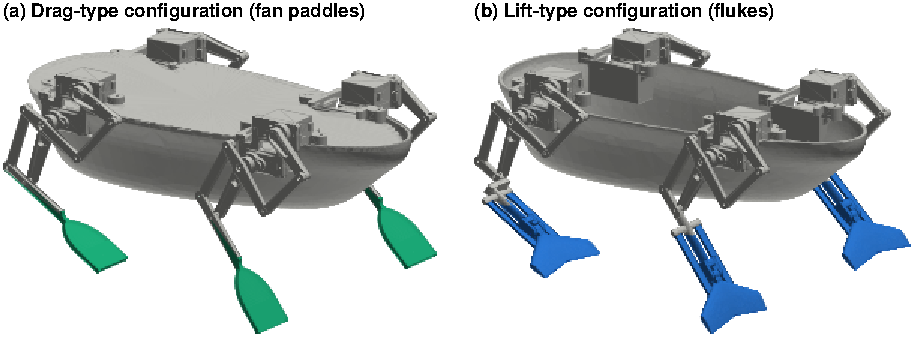
\includegraphics[width=\textwidth]{fig_robot}
  \caption[装配折扇桨与装配尾鳍的BODY2]{BODY2的两种游动构型，由CAD模型渲染而成。(a)阻力型构型，装有用于行走和划水的折扇桨（绿色）。(b)升力型构型，每条腿的直足杆上装有一个尾鳍（蓝色）。}
  \label{fig:robot}
\end{figure}

\section{推进器}
\label{sec:plat-propulsors}

\Cref{fig:propulsors}和\cref{tab:propulsors}对两种推进器进行了汇总。

\paragraph{阻力型：折扇桨。}足部是一个位于\SI{50}{\milli\metre}长杆末端、半径为\SI{42}{\milli\metre}的\SI{120}{\degree}扇面；\emph{扇面}（fan）仅指可折叠的叶片本身，\emph{桨}（paddle）则指叶片连同其杆。扇面张开时面积为\SI{18.5}{\square\centi\metre}（含杆为\SI{20.5}{\square\centi\metre}）。回程（recovery stroke）时由一根拉索将其折叠。在当前硬件中，折叠后的扇面宽度仍有\SI{30}{\milli\metre}（\SI{12.5}{\square\centi\metre}，为张开面积的68\,\%），因而空间不对称性较弱。\cref{sec:res-drag}中的优化冲程假设收拢宽度（folded width）为\SI{12}{\milli\metre}（\SI{5.9}{\square\centi\metre}）。扇面始终垂直于冲程方向；其开扇与合扇被视为两种刚性形状之间的瞬时切换（见\cref{sec:cfd-composite}）。

\paragraph{升力型：尾鳍。}尾鳍（设计方案“A2”）是一个小型后掠翼，展长（span）为\SI{60}{\milli\metre}，根弦长（root chord）为\SI{34}{\milli\metre}，平面面积（planform area）为\SI{11.2}{\square\centi\metre}，展弦比（aspect ratio）约为3.2。其截面为类似NACA\,0021的厚对称翼型。尾鳍通过靠近其前缘的销轴（pin）安装在直足杆的下端，从而可以绕展向轴俯仰（pitch）。在硬件上，俯仰是被动的，俯仰角由水动力矩与一片板簧（leaf spring）及两个限位（end stop）的约束共同决定。在本文的仿真中，俯仰角$\theta(t)$是给定的；被动尾鳍能在多大程度上跟随给定的俯仰规律，本文不作研究。

\begin{figure}[t]
  \centering
  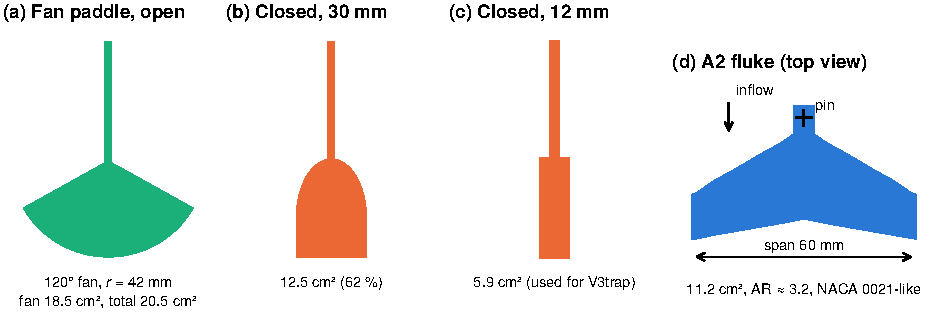
\includegraphics[width=\textwidth]{fig_propulsors}
  \caption[推进器几何形状]{CFD中使用的推进器几何形状，按比例绘制。(a)张开的折扇桨。(b)当前硬件的折叠扇面，宽\SI{30}{\milli\metre}。(c)优化冲程所假设的宽\SI{12}{\milli\metre}的折叠扇面。(d)尾鳍A2的俯视图及其销轴轴线。}
  \label{fig:propulsors}
\end{figure}

\begin{table}[t]
  \centering
  \caption[推进器参数]{推进器参数。面积为不含连杆的推进器平面面积。}
  \label{tab:propulsors}
  \small
  \begin{tabularx}{\textwidth}{@{}l>{\raggedright\arraybackslash}X>{\raggedright\arraybackslash}X@{}}
    \toprule
    & 折扇桨（阻力型） & 尾鳍A2（升力型） \\
    \midrule
    形状 & \SI{120}{\degree}扇面，$r=\SI{42}{\milli\metre}$，装于\SI{50}{\milli\metre}杆上 & 后掠翼，类似NACA\,0021 \\
    面积 & 张开时\SI{18.5}{\square\centi\metre}；折叠时\SI{12.5}{}或\SI{5.9}{\square\centi\metre}（宽30或12\,mm） & \SI{11.2}{\square\centi\metre} \\
    尺寸 & 扇面半径\SI{42}{\milli\metre} & 弦长\SI{34}{\milli\metre}，展长\SI{60}{\milli\metre} \\
    原理 & 阻力，折叠回程 & 升力，绕销轴俯仰 \\
    自由度 & $\psi,\phi$ + 开扇/合扇 & $\psi,\phi$ + 俯仰$\theta$ \\
    频率 & \SI{0.8}{\hertz}（机器人步态），\SI{1.39}{\hertz}（V3trap） & \SI{2}{\hertz} \\
    \bottomrule
  \end{tabularx}
\end{table}

\section{腿部运动}
\label{sec:plat-motions}

\Cref{fig:kinematics}给出了所研究的各种运动。

\paragraph{机器人步态。}机器人目前游动时采用的步态（gait）取自机器人的视频：周期为\SI{1.25}{\second}，$\mathrm{DUTY}=0.5$，髋关节做\SI{60}{\degree}的正弦摆动，回程时扇面折叠至\SI{30}{\milli\metre}。该步态原本是为行走而设计的，在此作为基准。

\paragraph{优化阻力型冲程（V3trap）。}\cref{sec:res-drag}中推导出的冲程周期为\SI{0.72}{\second}，$\mathrm{DUTY}=0.382$。髋关节以竖直方向为中心摆动\SI{50}{\degree}（\SIrange{120}{70}{\degree}），使桨几乎沿直线向后运动，并始终垂直于其运动路径。髋关节角速度遵循梯形规律，斜坡段约为\SI{45}{\milli\second}。回程时，平行四边形机构将桨向上卷收，扇面折叠至\SI{12}{\milli\metre}。扇面在$\tau_c=0.33$（即划水冲程减速段的起点）合扇，在$\tau_o=0$（即回程结束时的换向点）开扇（见\cref{fig:kinematics}a）。

\paragraph{尾鳍运动。}尾鳍腿保持髋关节固定，使足杆绕膝（knee）关节摆动，从而使尾鳍的销轴沿一段平缓的圆弧上下运动：摆角为$\pm\SI{24.9}{\degree}$，频率为\SI{2}{\hertz}，竖直行程为\SI{39.2}{\milli\metre}，峰值沉浮（heave）速度约为\SI{0.28}{\metre\per\second}（见\cref{fig:kinematics}b）。参考运动称为L0，取自整机Flare Live模型（见\cref{sec:cfd-flare}）：在\SI{0.223}{\metre\per\second}的航速下，控制尾鳍俯仰角以保持目标攻角（angle of attack），同时记录一条腿的关节角和尾鳍俯仰角，再对所记录的各周期进行相位平均。由此得到该航速下$|\alpha|$的第75百分位数为\SI{19.9}{\degree}。由L0派生出三个运动族：
\begin{itemize}
  \item \emph{L2，固定俯仰规律：}在\SIlist{0;0.08;0.15;0.30}{\metre\per\second}下保持L0运动不变，这与螺旋桨在固定转速、变进速条件下进行试验的做法相同。由于$\gamma$随$\U$变化（见\cref{eq:gammamax}），攻角在低速时较大，在高速时较小。
  \item \emph{L1，攻角规律：}根据沉浮速度计算俯仰规律，以保持目标$\alpha$：在\SI{0.223}{\metre\per\second}下为\SI{10}{\degree}或\SI{28}{\degree}，在\SI{0.40}{\metre\per\second}下为\SI{20}{\degree}。这些算例所用的铰链（hinge）轨迹与L0略有不同，因此并非严格意义上的攻角扫描。
  \item \emph{L3，随航速调度的俯仰（speed-scheduled pitch）：}采用L0的铰链轨迹和俯仰规律\eqref{eq:l3}，$\theta_0=\gamma_\text{max}/2$，航速为\SIlist{0.30;0.40}{\metre\per\second}（$\theta_0=\SI{21.6}{\degree}$和\SI{17.6}{\degree}）。
\end{itemize}

\begin{figure}[t]
  \centering
  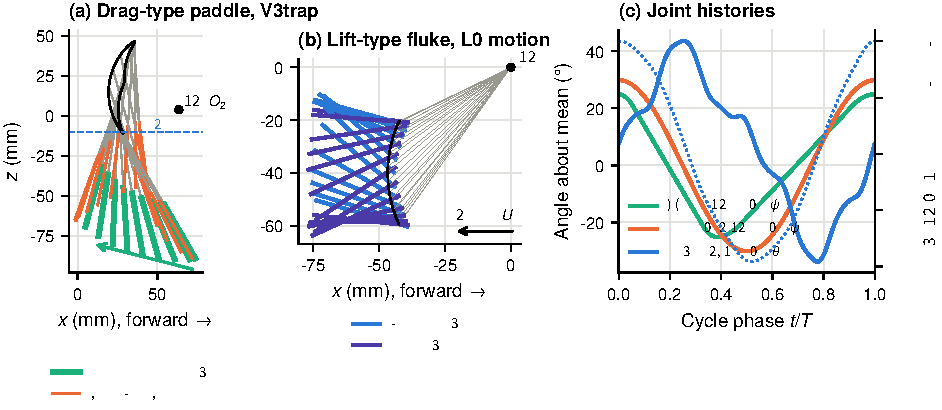
\includegraphics[width=\textwidth]{fig_kinematics}
  \caption[腿部运动]{船体坐标系中的腿部运动。(a)优化阻力型冲程V3trap：每个周期25个时刻的桨位置，包括张开（粗线）和合拢（细线）状态，以及连杆末端点$E$的轨迹。(b)尾鳍运动L0：一个周期内下行冲程和上行冲程的弦线位置，以及铰链轨迹。(c)关节时间历程：V3trap和机器人步态的髋关节角（相对于各自均值），以及L0的尾鳍俯仰角和铰链沉浮位移（点线，右轴）。}
  \label{fig:kinematics}
\end{figure}

这一设置本身决定了两种推进器之间存在两点差异，全文始终对此予以考虑。第一，两种推进器的面积（\SI{18.5}{}对\SI{11.2}{\square\centi\metre}）和频率均不同，因此本文同时报告单腿推力、单位面积推力和单位功率推力。第二，阻力型冲程经过了多轮优化，而L0是取自另一模型的运动，并未针对推力进行优化；L3是对尾鳍运动唯一的系统性改进。静止时，两种推进器每条腿所需的水动力输入功率（hydrodynamic input power）相近，为\SIrange{18}{22}{\milli\watt}，因此两者是在相近的功率预算下进行比较的。

\section{硬件样机}
\label{sec:plat-hw}

升力型构型已制成硬件（见\cref{fig:hardware}）。四条腿均装有打印制作的尾鳍，尾鳍安装在带板簧的被动销轴上。固件以每周期七个控制点驱动每条腿：大腿保持固定，足杆绕水平方向摆动$\pm\SI{25}{\degree}$，各腿按对角小跑（trot）协调。在\SI{2}{\hertz}下，这一运动与L0接近：销轴的竖直行程为\SI{38.0}{\milli\metre}（L0：\SI{39.2}{\milli\metre}），平均沉浮速度约为\SI{0.15}{\metre\per\second}（L0：\SI{0.157}{\metre\per\second}），但由于控制点之间以直线段连接，其峰值沉浮速度约低15\,\%。与仿真不同，硬件上的船体是反装的，因此机器人以钝端在前游动。在水中，装配尾鳍的BODY2明显比装配折扇桨、以当前步态游动时更快。\cref{sec:res-hw}将首次计时测试与自航估计进行比较。优化后的桨未作测试，因为它需要可控的折叠和梯形速度规律，而现有硬件不具备这些条件。

\begin{figure}[t]
  \centering
  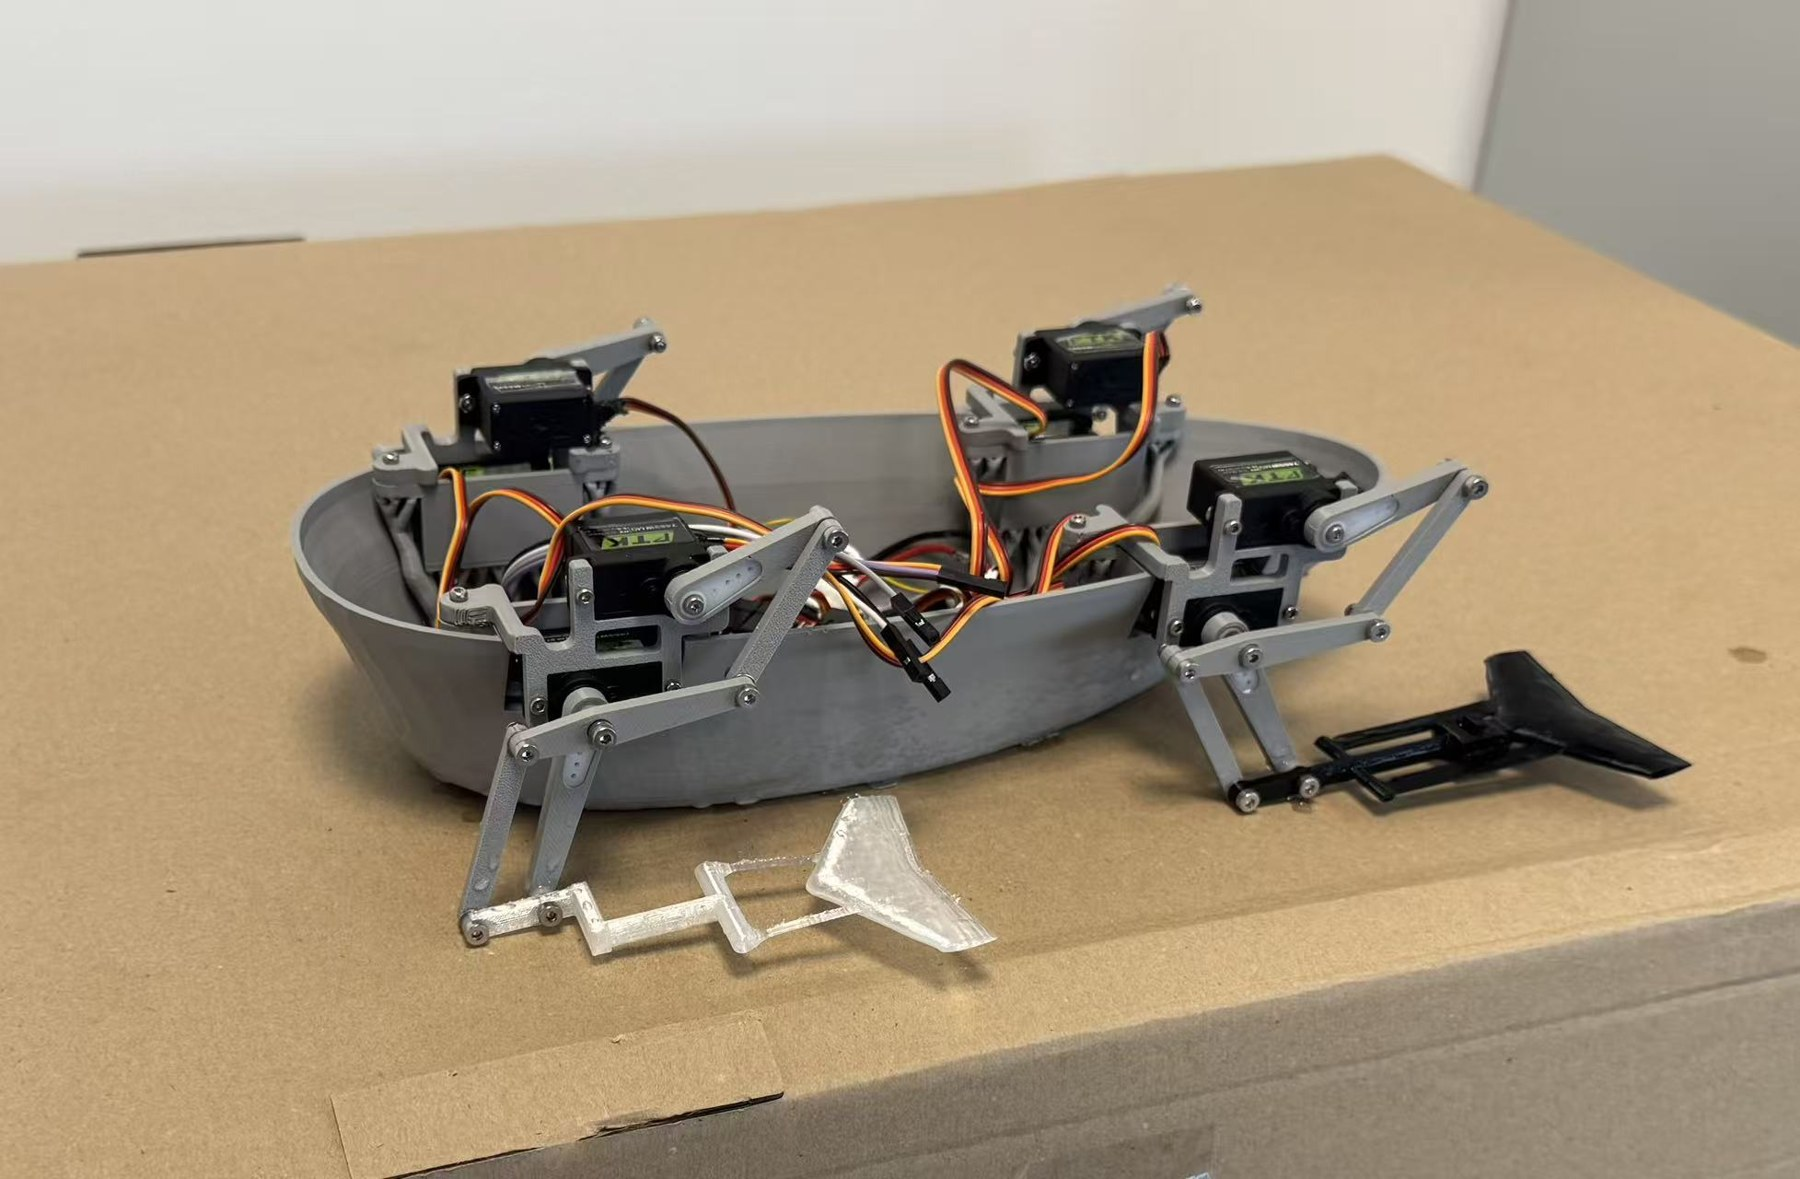
\includegraphics[width=0.78\textwidth]{fig_hardware.jpg}
  \caption[装配尾鳍的BODY2硬件]{BODY2的硬件样机，打印制作的尾鳍脚安装在腿部连杆上；图中另有两只尾鳍脚放在桌面上。每条腿由两个PTK\,7465W舵机驱动。}
  \label{fig:hardware}
\end{figure}

\chapter{基于降阶模型的步态优化}
\label{ch:mujoco}

本章回答RQ1。在MuJoCo~\cite{Todorov2012}中建立一个各连杆受准定常（quasi-steady）力作用的整机模型，并在执行器约束和姿态约束下用CMA-ES~\cite{Hansen2001,Hansen2016}优化其步态。该模型的计算代价足够低，可进行数千次评估，但其系数未经标定。其目的在于揭示优化器会选择哪种推进原理，以及这一答案如何取决于模型所包含的物理，而不是预测BODY2的速度。

\section{模型}
\label{sec:mj-model}

\subsection{机器人}

BODY2无法直接使用：由CAD导出的模型是一棵开链运动学树（kinematic tree），其中的平行四边形连杆并未闭合，而且其浮力分布尚未测量。因此，优化采用一个尺寸相近的简化四足模型\texttt{toy\_quad}（\cref{fig:mj-model}、\cref{tab:mj-robot}）。每条腿有三个绕横轴的铰链关节：髋、膝和脚蹼腕关节，共计十二个执行器。脚蹼为\qtyproduct{52 x 36}{\milli\metre}的薄板，其面积\SI{18.7}{\square\centi\metre}与BODY2张开状态下折扇桨的面积相近；全文将其称为\emph{脚蹼}（flipper），以区别于真实机器人的折扇桨和尾鳍：根据所包含的物理，它既可划水也可拍动，而BODY2的两种推进器各自只针对一种原理而设计。干质量为\SI{0.78}{\kilo\gram}；完全浸没时，机器人的排水体积为\SI{1126}{\cubic\centi\metre}，因此它像BODY2一样漂浮在水面上。体长\SI{0.239}{\metre}用于将速度表示为每秒体长数（body lengths per second）。

\begin{figure}[t]
  \centering
  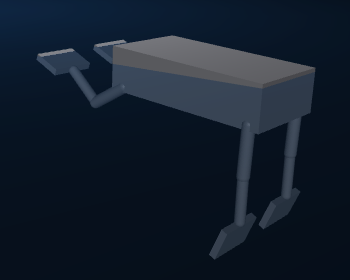
\includegraphics[width=0.42\textwidth]{fig_mj_model.png}
  \caption[MuJoCo模型]{漂浮在水面上的MuJoCo模型\texttt{toy\_quad}（仿真渲染图）。每条腿有一个髋关节、一个膝关节和一个脚蹼关节。}
  \label{fig:mj-model}
\end{figure}

\begin{table}[t]
  \centering
  \caption[MuJoCo机器人模型]{降阶（reduced-order）机器人模型\texttt{toy\_quad}。}
  \label{tab:mj-robot}
  \small
  \begin{tabular}{@{}llll@{}}
    \toprule
    部件 & 几何形状 & 尺寸 & 质量 \\
    \midrule
    躯干 & 长方体 & \qtyproduct{0.20 x 0.10 x 0.05}{\metre} & \SI{0.600}{\kilo\gram} \\
    大腿（$\times4$） & 胶囊体 & $r=\SI{7}{\milli\metre}$, $l=\SI{55}{\milli\metre}$ & \SI{0.020}{\kilo\gram} \\
    小腿（$\times4$） & 胶囊体 & $r=\SI{6}{\milli\metre}$, $l=\SI{50}{\milli\metre}$ & \SI{0.015}{\kilo\gram} \\
    脚蹼（$\times4$） & 板 & \qtyproduct{8 x 52 x 36}{\milli\metre} & \SI{0.010}{\kilo\gram} \\
    \midrule
    \multicolumn{4}{@{}l}{关节范围：髋和膝$\pm\SI{1.3}{\radian}$，脚蹼$\pm\SI{1.6}{\radian}$；
      腿位于$\pm\SI{0.085}{\metre}$（前后向）、$\pm\SI{0.045}{\metre}$（横向）处} \\
    \multicolumn{4}{@{}l}{干质量\SI{0.78}{\kilo\gram}；附加质量\SI{0.28}{\kilo\gram}；体长
      \SI{0.239}{\metre}；时间步长\SI{2}{\milli\second}，隐式积分器} \\
    \bottomrule
  \end{tabular}
\end{table}

\subsection{水动力}

每个几何体$k$受到一个准定常力，该力按其浸没比例$f_k$缩放，并作用于其中心：
\begin{equation}
  \bm F_k = \rho g V_k f_k\,\bm e_z
  \;-\; \tfrac12\rho f_k \sum_{i=1}^{3} C_{D,i} A_i\, v_i|v_i|\,\bm e_i
  \;-\; c_v f_k\,\bm v \;+\; \bm L_k .
  \label{eq:mj-force}
\end{equation}
式中，$\bm v$为物体中心相对于静水的速度，$v_i$为其沿体轴$\bm e_i$的分量，$A_i$为投影面积；$c_v$为一个很小的线性阻尼系数（脚蹼、连杆和躯干分别为0.05、0.02和\SI{0.10}{\newton\second\per\metre}），仅在速度很低时起作用。阻力是各向异性（anisotropic）的：脚蹼在板面法向和沿板面方向上的$C_D=(2.2,\,0.10,\,0.10)$，连杆为$(0.5,0.5,0.25)$，躯干为$(0.9,1.6,1.8)$。在纯阻力（drag-only）模型中，这种各向异性是推力的唯一来源。浸没比例根据每个物体实际的竖直范围计算，因此露出水面的脚蹼会失去其受力。附加质量（added mass）$m_a=C_a\rho V$（脚蹼$C_a=1.0$，连杆为0.3，躯干为0.2）被计入物体惯量，同时施加一个恒定的向上力$m_a g$以抵消其重量。与显式的$\dot{\bm v}$项不同，这种各向同性近似是无条件稳定的。这些系数为文献值，与河狸机器人模型\cite{Chen2021,Chen2022}中的取值处于同一水平；它们未经标定。

\paragraph{升力。}式~\eqref{eq:mj-force}中除$\bm L_k$以外的所有项都与相对流动的某一分量方向相反。脚蹼上可选择性地施加一个失速后平板升力（post-stall flat-plate lift）：
\begin{equation}
  C_L(\alpha) = c_l \sin 2\alpha, \qquad |\bm L| = \tfrac12\rho\,C_L\,A_\text{face}|\bm v|^2 f,
  \label{eq:mj-lift}
\end{equation}
其方向垂直于$\bm v$，位于$\bm v$与板法线所张成的平面内，其中$\alpha$为$\bm v$与板面之间的夹角。$c_l=1.1$是教科书中的平板取值，未作展弦比（aspect ratio）修正。在小$\alpha$时，升力随$\alpha$增长，而阻力随$\alpha^2$增长，因此快速、浅角度、顺桨的划动在纯阻力模型中几乎不产生推力，而在含升力时则产生很大的推力。关闭升力后，升力型步态不可能胜出，因为使其胜出的机制并不存在。

\paragraph{推力分解。}为识别步态的推进机制，在评分窗口内分别累积升力项和阻力项（包括线性项）沿游动方向的带符号冲量。升力冲量为正、阻力冲量为负的步态称为\emph{升力推进的}（lift-propelled）：升力提供向前的冲量，而阻力只起阻碍作用。该分解通过滑行试验（coasting test）进行了检验，在该试验中初始动量等于各冲量之和。为量化升力在推进中所占的份额，定义\emph{升力推力占比}（lift thrust share）
\begin{equation}
  s_L = \frac{I_L}{|I_\text{trunk}|}
  \label{eq:liftshare}
\end{equation}
即升力项的前向冲量$I_L$与躯干阻力冲量之比；腿部自身的阻力冲量单独累计。划水型划动的$s_L\approx0$；升力推进的划动$s_L>1$，因为升力还需克服腿部自身的阻力。该占比也可作为附加限值$s_L\le s_\text{max}$，从而在含升力的模型中强制出现阻力型划动（\cref{sec:mj-liftshare}）。

\subsection{舵机模型}
\label{sec:mj-servo}

执行器为位置控制舵机，刚度为\SI{60}{\newton\metre\per\radian}，采用临界阻尼。实际的航模舵机无法以任意快的速度运动。因此，为每个执行器赋予直流电机的力矩--转速特性：
\begin{equation}
  \tau = \tau_s\,u - \frac{\tau_s}{\omega_\text{max}}\,\omega, \qquad |u|\le1,
  \label{eq:servo}
\end{equation}
其中堵转力矩（stall torque）$\tau_s=\SI{3}{\newton\metre}$，空载转速（no-load speed）$\omega_\text{max}=\SI{400}{\degree\per\second}$。这些取值是在确定BODY2所用舵机之前选定的；PTK\,7465W的堵转力矩更低、空载转速更高（\cref{sec:plat-robot}），其影响在\cref{sec:disc-limits}中讨论。反电动势（back-EMF）项是一个黏性阻尼$b=\tau_s/\omega_\text{max}\approx\SI{0.43}{\newton\metre\second\per\radian}$，它被加入关节阻尼，并由MuJoCo隐式积分；结果与时间步长无关。两种更简单的方案均告失败：仅限制指令的变化率时，腿会被向后拖动，然后以\SI{1500}{\degree\per\second}的速度猛然弹向前方；而在每一步重写力矩限值则相当于一个显式阻尼，会以高达\SI{3000}{\degree\per\second}的速度振荡，并使结果随时间步长相差六倍。

本章报告两种功率度量。优化采用电机轴上的平均机械功率$\sum_j\langle|\tau_{m,j}\,\omega_j|\rangle$，其中电机力矩$\tau_m=\tau-b\,\omega$，且不回收制动能量。电功率在此基础上加上同一电机模型的铜损（copper loss），即$\sum_j\langle\max(\tau_{m,j}\omega_j,0)+\tau_{m,j}^2\,\omega_\text{max}/\tau_s\rangle$，它由式~\eqref{eq:servo}得出，无需引入新参数；电功率在优化完成后计算，用作校核。本章中的运输代价（cost of transport）为功率除以速度，单位为\si{\joule\per\metre}。

\section{步态参数化}
\label{sec:mj-gait}

每个执行器$i$跟踪如下目标角度：
\begin{equation}
  q_i(t) = q_{0,i} + r(t)\sum_{h=1}^{H} A_{i,h}\,\sin\!\big(h\,\vartheta(t)+\varphi_{i,h}\big), \qquad H=2,
  \label{eq:gait}
\end{equation}
其中$q_{0,i}$为偏置，$A_{i,h}$为幅值，$\varphi_{i,h}$为相位，$r(t)$为在前\SI{1.5}{\second}内从0升至1的斜坡函数。占空比扭曲（duty warp）$\vartheta(t)$使划水冲程可以快于或慢于回程，同时保持周期不变：设周期进度为$c=(ft)\bmod1$，则
\begin{equation}
  \vartheta = \begin{cases}
    \pi\,c/\mathrm{DUTY}, & c<\mathrm{DUTY},\\
    \pi + \pi\,(c-\mathrm{DUTY})/(1-\mathrm{DUTY}), & c\ge\mathrm{DUTY}.
  \end{cases}
  \label{eq:duty-warp}
\end{equation}
二次谐波在$\pi$相移下保持不变，可用于表达脚蹼的顺桨（feathering）。它并不是产生净推力的必要条件：单一谐波就已能推动模型前进。同类关节共享幅值和偏置。搜索范围为$f\in[0.2,2.5]$\,Hz、$\mathrm{DUTY}\in[0.25,0.75]$、$A\in[0,0.9]$\,rad和$q_0\in[-0.5,0.5]$\,rad，并归一化到$[0,1]$。

腿间协调方式要么是自由的，即每个执行器具有独立的相位（35个参数），要么固定为某一\emph{步态族}（gait family），即每类关节一个相位（17个参数）。各步态族由每条腿相对于左前腿FL的延迟定义，该延迟在占空比扭曲之前施加于时间上：
\begin{center}
  \small
  \begin{tabular}{@{}lll@{}}
    \toprule
    步态族 & 通用名称 & FR、BL、BR的延迟（占周期的比例） \\
    \midrule
    \texttt{diag} & 对角小跑（trot） & 0.5, 0.5, 0 \\
    \texttt{lr} & 同侧步（pace） & 0.5, 0, 0.5 \\
    \texttt{fb} & 跳跃步（bound） & 0, 0.5, 0.5 \\
    \texttt{wave} & 行走步（walk） & 0.5, 0.75, 0.25 \\
    \texttt{inphase} & 四足齐跳（pronk） & 0, 0, 0 \\
    \bottomrule
  \end{tabular}
\end{center}
为对自由步态进行分类，将一次谐波幅值最大的那类关节的延迟与各步态族进行比较，并报告平均圆周距离（circular distance）最小的步态族及该距离（0表示相同，0.5表示相反）。

\section{目标函数、约束与优化器}
\label{sec:mj-objective}

每次评估先让机器人静置稳定\SI{1.0}{\second}，再在\SI{1.5}{\second}内逐步引入步态，然后对随后的\SI{8}{\second}进行评分，该时长向上取整为完整的划动周期。速度定义为沿初始航向的位移除以窗口长度，因此转向会被自动惩罚。本章采用两种目标：最高速度，或在最低速度$v_\text{min}$约束下的最低平均机械功率。全部设置列于\cref{tab:app-mujoco}。

稳定性通过限值而非权重来施加。设航向误差、横滚和俯仰的均方根（RMS）值及其限值为$\ell_k$，则惩罚项为
\begin{equation}
  p = \sum_k \frac{\max(0,\mathrm{RMS}_k-\ell_k)}{\ell_k}
    \;\big[+\,\text{出水项与}\,v_\text{min}\,\text{项}\big], \qquad
  \text{适应度} = \begin{cases} \text{目标值}, & p=0,\\ -1000-p, & p>0. \end{cases}
  \label{eq:feasibility}
\end{equation}
因此，任何不可行步态的得分都低于所有可行步态；速度无法弥补对限值的违反。早先对速度和姿态采用加性加权的做法，在腿可以自由运动后便失效了：速度占据主导，最优步态的横滚达\SI{42}{\degree}，偏航达\SI{44}{\degree}。共使用两组限值：适中限值，即航向/横滚/俯仰为$10/10/\SI{15}{\degree}$，用于本章；以及严格限值，即$10/5/\SI{5}{\degree}$，用于\cref{app:coord}中的腿间协调研究。在特别说明之处，任一肢体浸没不足一半的时间占比（出水，surfacing）被限制在5\,\%以内，因为该模型不包含自由液面物理。

优化器为CMA-ES，种群规模为16，在归一化空间中的初始步长为0.25；除非另有说明，每次运行2500次评估，每种条件使用多个随机种子（seed）。每个结果都是模型所允许范围的一个界：对最高速度而言是下界，对最低功率而言是上界。数值以各种子上的均值$\pm$标准差给出。

\section{结果}
\label{sec:mj-results}

\subsection{基线与舵机限制}

一个手工设计的\SI{1.2}{\hertz}对角小跑步态以\SI{0.070}{\metre\per\second}（每秒0.29个体长）的速度游动，俯仰RMS为\SI{26.7}{\degree}，舵机在85\,\%的时间内处于饱和。在没有舵机模型时，优化器找到的步态关节速度为\SIrange{2700}{4200}{\degree\per\second}，约为舵机限值的七到十倍。在加入舵机模型后重放，其中最好的步态并不向前运动（\SI{-0.001}{\metre\per\second}）。在含舵机模型的条件下重新优化后，三次自由相位（free phase）搜索达到\SIrange{0.11}{0.25}{\metre\per\second}，且均接近某一边界。因此，舵机限制必须纳入模型；以下所有结果均包含该限制。

\subsection{等速条件下阻力与升力的比较}

比较两种物理模型下的最快步态是不公平的，因为功率随速度急剧上升，而各最快步态的速度并不相同。因此，比较在等速条件下进行：在适中限值且出水比例不超过5\,\%的条件下，针对五个步态族和两个种子，求达到$v_\text{min}\in\{0.10,0.20,0.30\}$\,m/s所需的最低机械功率（\cref{tab:mj-pareto}、\cref{fig:mj-pareto}）。

\begin{table}[t]
  \centering
  \caption[等速下的最低功率：阻力与升力对比]{达到所需速度的最低平均机械功率，适中限值，取五个步态族和两个种子中的最优值（括号内为最优解所属的步态族，以及十次搜索中可行的次数）。左：不含升力模型中的阻力型划动；中：在含升力模型中以$s_L\le0.1$强制的阻力型划动（\cref{sec:mj-liftshare}）；右：含升力模型中不加约束的划动。}
  \label{tab:mj-pareto}
  \small
  \begin{tabular}{@{}cccc@{}}
    \toprule
    所需速度 & 纯阻力模型 & 升力模型，$s_L\le0.1$ & 升力模型，无约束 \\
    \midrule
    \SI{0.10}{\metre\per\second} & \SI{0.23}{\watt}（行走步） & \SI{0.42}{\watt}（跳跃步；2/10） & \SI{0.10}{\watt}（跳跃步；10/10） \\
    \SI{0.20}{\metre\per\second} & \SI{1.04}{\watt}（跳跃步） & \SI{5.50}{\watt}（四足齐跳；1/10） & \SI{0.55}{\watt}（四足齐跳；8/10） \\
    \SI{0.30}{\metre\per\second} & \SI{3.10}{\watt}（对角小跑） & 无（0/10） & \SI{0.97}{\watt}（跳跃步；4/10） \\
    \bottomrule
  \end{tabular}
\end{table}

有三项结果是稳健的。第一，只要模型中包含升力且未被压制，每个可行最优解都是升力推进的：在本实验全部22个含升力的可行最优解中，升力冲量均为正（前沿上为\SIrange{0.46}{2.2}{\newton\second}），阻力冲量均为负。只要能够拍动，优化器就从不划水。第二，在全部三个速度下，等速条件下升力推进步态所需的功率约为最佳纯阻力步态的二分之一到三分之一。第三，每个最优解都依赖于其所在的物理模型：去除升力后，升力最优解仅保留其速度的35--58\,\%；而加入升力后，27个阻力最优解中有26个不再满足姿态限值，因为升力还会对躯干产生力矩（\cref{sec:mj-liftshare}）。该比值的大小并不可靠：搜索尚未收敛（第二个种子将\SI{0.20}{\metre\per\second}下的纯阻力功率从2.99降至\SI{1.04}{\watt}），因此两条前沿均为上界。若改用计入舵机铜损的电功率，排序同样不变：纯阻力前沿所需功率分别为0.22、1.14和\SI{2.80}{\watt}，升力前沿分别为0.10、0.47和\SI{0.86}{\watt}。

\begin{figure}[t]
  \centering
  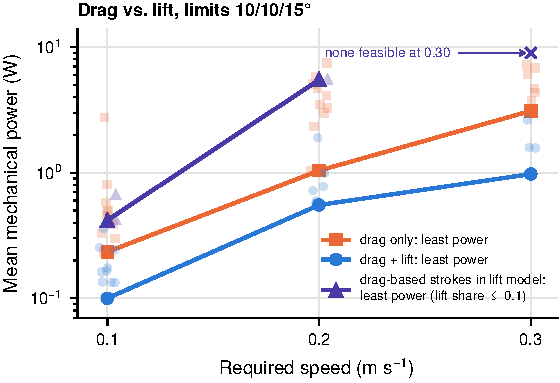
\includegraphics[width=0.62\textwidth]{fig_mj_pareto}
  \caption[等速下的最低功率]{达到所需速度的最低机械功率，适中限值：纯阻力模型、含升力模型，以及在含升力模型中以$s_L\le0.1$强制的阻力型划动。浅色标记为各步态族和各种子的单个最优解。}
  \label{fig:mj-pareto}
\end{figure}

\subsection{升力模型内的阻力型划动}
\label{sec:mj-liftshare}

\Cref{tab:mj-pareto}中纯阻力模型与升力模型之间的比较，既是两种推进原理的比较，也在同等程度上是两个模型的比较。对RQ1更直接的检验是在同一模型内比较两种原理。为此，在升力模型的最低功率搜索中加入附加限值$s_L\le0.1$（见式\eqref{eq:liftshare}），只允许从阻力获得推力的划动，速度、限值、步态族和种子均与不加约束的搜索相同（共30次搜索）。

结果见\cref{tab:mj-pareto}的中间一列和\cref{fig:mj-pareto}。30次搜索中只有3次找到了可行的阻力型划动；其余大多满足占比限值，但达不到所需速度。基于这一有限的样本，阻力型划动在\SI{0.10}{\metre\per\second}时所需功率为升力推进划动的4.2倍（\SI{0.42}{}对\SI{0.10}{\watt}），在\SI{0.20}{\metre\per\second}时为10倍（\SI{5.50}{}对\SI{0.55}{\watt}）；没有任何阻力型划动能达到\SI{0.30}{\metre\per\second}，最接近的只达到\SI{0.26}{\metre\per\second}。可行域很窄，因此该倍数中可能有一部分源于搜索困难而非物理本身；在两个种子、2500次评估的条件下，方向是可靠的，但数值并不可靠。

两种比较给出了答案的上下界。在纯阻力模型中，划水型划动无须压制其脚蹼本应产生的升力，这对它有利；在升力模型中则必须压制，而且带约束的搜索很困难，这对它不利。综合来看，在该模型中阻力型划动在相同速度下所需功率约为升力型划动的二至十倍，并且达不到升力推进步态仍能巡航的速度。

另一项补充检验将纯阻力模型的27个可行最优解在开启升力的条件下重新仿真（回放）。其中21个的升力推力占比超过0.1（中位数1.26），即一旦存在升力，同样的腿部动作主要依靠升力推进；26个不再保持直行和平稳。因此，一个划动是阻力型还是升力型，在同等程度上取决于物理模型和动作本身：只要脚蹼斜着划过水，无论模型是否包含升力，它都会产生升力。在纯阻力模型中找到的划水型划动不能原样搬到真实脚蹼上。

\section{小结}
\label{sec:mj-summary}

在该模型范围内，RQ1的答案在方向上是明确的。当物理模型包含升力且升力未被压制时，优化器在全部101个可行最优解（本章22个，其余来自\cref{app:coord}中的腿间协调研究）中都选择了升力推进的划动。在等速条件下，其所需功率为纯阻力模型中最佳划动的二分之一到三分之一；而在升力模型内强制采用阻力型划动时，少数可行的划动（30次搜索中的3次）所需功率为升力推进划动的四至十倍，且达不到\SI{0.30}{\metre\per\second}；因此在该模型中，阻力型划动的代价至少约为升力型的两倍，最高可达十倍。划动属于阻力型还是升力型取决于物理模型：纯阻力模型中的大多数划水型划动在加入升力后变为升力推进。哪种腿间协调方式最优是另一个问题，它主要取决于姿态限值，见\cref{app:coord}。有三点注意事项将上述结论限定在该模型之内：系数和升力斜率未经标定；尽管脚蹼的$\mathit{AR}\approx1.4$，平板升力却未作展弦比修正；且搜索未完全收敛，尤其是针对阻力型划动的带约束搜索。因此，\Cref{ch:cfd,ch:results}将通过对真实腿部的流场解析仿真（resolved flow simulations），检验这一核心论断，即升力型拍动优于阻力型划水。

\chapter{流动仿真方法}
\label{ch:cfd}

本文使用了两种流动求解器。基于OpenFOAM的单腿仿真解析单个推进器（propulsor）周围的流动，
并提供\cref{ch:results}中的推力（thrust）与功率数据。采用实时格子玻尔兹曼（lattice Boltzmann）求解器Flare Live进行的整机仿真，
则提供尾鳍的参考运动以及自由游动机器人的定性趋势（\cref{app:flare-trends}）。本章对二者分别加以介绍。

\section{基于重叠网格的单腿CFD}
\label{sec:cfd-of}

\subsection{控制方程与求解器}

水（$\rho=\SI{1000}{\kilo\gram\per\cubic\metre}$，$\nu=\SI{1.0e-6}{\square\metre\per\second}$）的流动被建模为不可压缩、层流、单相流动。
雷诺数为$10^3$--$10^4$（见\cref{sec:fund-forces}），处于层流至转捩的范围，在该范围内作用力主要由边缘处的分离涡主导；
本文不使用湍流模型。不可压缩Navier--Stokes方程采用OpenFOAM v2606 \cite{Weller1998}中的\texttt{overPimpleDyMFoam}求解，
该求解器是一种有限体积（finite-volume）求解器，采用PIMPLE压力--速度耦合（pressure--velocity coupling）以及重叠网格（overset/Chimera grid）\cite{Windt2020}。
时间步长按最大库朗数（Courant number）0.8自适应调整。

之所以选用重叠网格，是因为推进器在每个周期内相对于船体（hull）的转角可达\SI{120}{\degree}。
贴体（body-fitted）的部件网格（component mesh）在静止的背景网格（background mesh）内随推进器作刚体运动。
在每个时间步中，被推进器覆盖的背景网格单元被移除，即挖洞（hole cutting），各网格上的解通过插值边界单元（fringe cells）处的插值相互耦合。
计算采用反距离（inverse-distance）插值模板（stencil）；对于部分算例，计算在模板更新时崩溃，
这些算例随后改用跟踪式反距离（tracking inverse-distance）变体，从最后一次保存的时刻继续计算。
为防止挖洞失败，在第一个时间步中检查洞单元的数量，若其超过全部单元的3\,\%或少于50个，则换用另一种模板重新启动该算例。

\subsection{计算域、边界条件与运动}

仿真在随船体运动的参考系中进行。前进速度$\U$以均匀来流的形式从上游边界进入；
下游边界采用固定压力，速度采用入口--出口（inlet--outlet）条件。
计算域顶部为位于尾鳍（fluke）上方\SI{12}{\centi\metre}处的滑移壁面（slip wall），即代表无自由液面（free surface）深水的刚性盖（rigid lid）；
侧面和底部边界同样为远离推进器的滑移壁面。推进器的刚体运动以位置与姿态数据表的形式给定，数据来自\cref{sec:plat-motions}中的腿部运动学。
为避免突然启动引起的压力尖峰和时间步长骤减，尾鳍运动从静止开始，在前半个周期内以平滑阶跃过渡。
共仿真三个周期；尾鳍取后两个周期的平均值，折扇桨（fan paddle）取第三个周期的平均值。

仅对推进器本身进行仿真：尾鳍不含其脚杆，折扇桨包含其\SI{3}{\milli\metre}的细杆，但不含曲柄（crank）和平行四边形（parallelogram）机构。
连杆（linkage）只贡献阻力，假定该阻力对两种推进器相同，并已计入自航（self-propulsion）平衡的阻力项中（见\cref{sec:res-selfprop}）。
细杆约贡献桨推力的1\,\%。此外，\cref{sec:res-selfprop}中使用的船体阻力取自另行开展的含自由液面的裸船体两相流仿真，此处不再详述。

\subsection{网格}

两套网格均由推进器表面通过\texttt{snappyHexMesh}生成。对于尾鳍，采用经过清理的CFD几何：
去除打印件上的销轴（pin）孔和限位（end stop）臂，并将\SI{0.1}{\milli\metre}的尾缘在95\,\%弦长（chord）处截断，
因为这些细节会产生退化网格单元，使时间步长降至\SI{e-4}{\second}以下。
由此得到的鳍片与Flare几何之间偏差的中位数为\SI{0.12}{\milli\metre}。网格参数列于\cref{tab:meshes}。

\begin{table}[t]
  \centering
  \caption[网格参数]{单腿仿真的网格参数。尺寸为推进器周围加密区域内的网格单元边长。}
  \label{tab:meshes}
  \small
  \begin{tabular}{@{}lccc@{}}
    \toprule
    & 尾鳍（L算例） & 折扇桨（D算例） & 确认用翼型 \\
    \midrule
    部件网格（表面） & \SI{1.2}{\milli\metre}（\SI{0.6}{\milli\metre}） & \SI{2.5}{\milli\metre}（\SI{1.25}{\milli\metre}） & \SI{2.5}{\milli\metre} \\
    背景网格 & \SI{2.5}{\milli\metre} & \SI{4}{\milli\metre} & \SI{5}{\milli\metre} \\
    单位长度表面网格数 & 每弦长$\approx50$ & 每半径$\approx34$ & 每弦长$\approx40$ \\
    单元数，部件+背景 & $1.8\times10^5+5.4\times10^5$ & -- & -- \\
    仿真周期数/平均周期数 & 3 / 2 & 3 / 1 & 3 / 2 \\
    启动方式 & 0.5周期平滑阶跃 & 无 & 无 \\
    \bottomrule
  \end{tabular}
\end{table}

折扇桨网格比尾鳍网格粗。该网格建立较早，当时正在设计桨的冲程，为保持各轮桨设计迭代之间的可比性而沿用至今。
其对比较结果的影响在\cref{sec:ver-drag}中讨论。

\subsection{折扇的两态合成}
\label{sec:cfd-composite}

对折扇的折叠过程进行仿真需要可变形几何。作为替代，每个桨冲程以相同的运动仿真两次：一次为开扇状态，一次为合扇状态。
随后由这两次计算组合得到周期力时程，
\begin{equation}
  \bm F(\tau) = \begin{cases}
    \bm F_\text{open}(\tau), & \tau_o \le \tau < \tau_c,\\
    \bm F_\text{closed}(\tau), & \text{其他情况},
  \end{cases}
  \label{eq:composite}
\end{equation}
式中$\tau$为周期相位，$\tau_o,\tau_c$分别为开扇相位和合扇相位（\cref{fig:composite}）。
因此，开扇与合扇均为瞬时完成，且每次计算各自保留自身的尾流。该两态合成（two-state composite）是折叠过程的一阶模型。
其优点在于，可在仿真完成后对任意$(\tau_o,\tau_c)$组合评估折叠时机，且无需额外计算代价。
该方法存在两项系统误差，二者均使结果偏于乐观。

\paragraph{忽略附加质量（added mass）的变化。}扇面张开时，其周围的水必须被带动起来；扇面合拢时，这部分水被释放。
在式\eqref{eq:composite}中，开扇计算开始时的流场是在扇面张开状态下已经建立起来的流动，而合扇计算结束时无需释放任何东西。
记扇面在水体参考系中的速度为$V$（向前为正），开扇与合扇状态下附加质量之差为$\Delta m_a$，
则每个周期内桨上缺失的冲量介于两个极限之间：
\begin{equation}
  \Delta J = \begin{cases}
    \Delta m_a\,(V_c - V_o) & \text{势流：释放的动量返回到桨上，}\\
    -\Delta m_a\,V_o & \text{完全脱落：释放的动量留在尾流中，}
  \end{cases}
  \label{eq:addedmass}
\end{equation}
式中$V_o$和$V_c$分别为开扇和合扇时刻的速度。在分离流中，释放的动量有一部分以停止涡（stopping vortex）的形式脱落（shedding），
因此真实值介于两个极限之间；开扇代价$-\Delta m_a V_o$则没有这样的出路，在两个极限中均存在。
修正后的平均推力以$\Tm+\Delta J/T$在两个极限下的取值范围给出。
开扇状态的附加质量由$\U=0$时开扇桨仿真的加速阶段辨识得到：将$F_x=-m_a\dot v_x-\tfrac12\rho C_N S\,v_x|v_x|$拟合到力时程上，
根据拟合窗口和参考点的不同，得到$m_a=\SIrange{38}{49}{\gram}$，与同面积圆盘的\SI{38}{\gram}相近。
扇面折叠至\SI{12}{\milli\metre}时附加质量约为\SI{5}{\gram}，据此对V3trap取$\Delta m_a=\SI{38}{\gram}$，
对机器人步态取\SI{20}{\gram}，因为后者的扇面仅折叠至\SI{30}{\milli\metre}；$\Delta m_a$的不确定度约为$\pm15$\,\%。
若扇面在船体参考系中处于静止时切换状态，则该修正在此参考系中不做功，功率$\Pm$亦不作修正。V3trap在$\tau_c=0.33$时合扇，此时扇面仍在运动；相应的功每个周期约为$\tfrac12\Delta m_a V_c^2$量级，未计入$\Pm$。

由此得出两点推论。其一，在髋部运动的换向点处切换（此时$V$等于前进速度$\U$），在$\U=0$时无需修正，
但在有航速时每个周期需付出$\Delta m_a\U$的代价。其二，若在换向之前、即回程（recovery）的减速阶段开扇，
则合成模型会将张开的扇面在减速过程中释放的动量计入桨上，却不计入其先前带动这部分水所付出的代价。
因此，该合成模型会人为地偏向提前开扇；本文中所有桨的结果均采用$\tau_o=0$。

\paragraph{开扇计算的尾流。}在划水冲程（power stroke）中，开扇桨计算会穿过其自身开扇回程所产生的尾流，而该回程已将水向前推动；
真实的桨以折叠状态回程，留下的尾流要弱得多。这使合成模型中划水冲程的相对速度偏高。
该效应未作量化，列为局限性之一。

\begin{figure}[t]
  \centering
  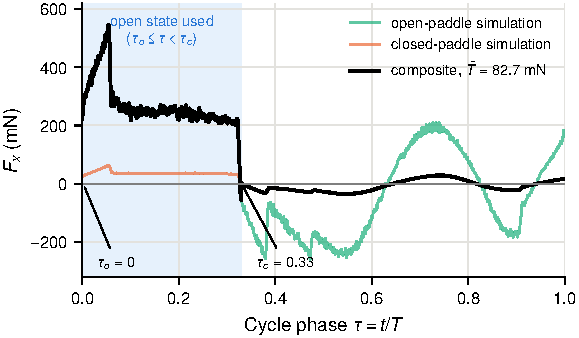
\includegraphics[width=0.62\textwidth]{fig_composite}
  \caption[两态合成]{V3trap在$\U=0$时折扇桨的两态合成。在$\tau_o=0$与$\tau_c=0.33$之间（阴影区域）采用开扇桨仿真结果，
    周期其余部分采用合扇桨仿真结果。在进行式\eqref{eq:addedmass}的附加质量修正之前，
    该合成结果的周期平均推力为\SI{82.7}{\milli\newton}。}
  \label{fig:composite}
\end{figure}

\subsection{后处理}

在每个时间步中，对推进器表面上的压力和黏性力进行积分，力矩取关于髋轴$O_2$的值。
推力、输入功率（input power）和效率由式\eqref{eq:thrust}至\eqref{eq:eta}求得，其中尾鳍销轴或桨参考点的速度以及角速度取自运动表。
关于尾鳍销轴的俯仰力矩给出了俯仰执行器或弹簧所需提供的铰链（hinge）力矩。
攻角由式\eqref{eq:alpha}根据销轴速度和俯仰角计算，并以两种方式之一给出：一是周期内$|\alpha|$的第75百分位数$\alpha_{75}$，
二是每个半冲程中间部分（远离冲程换向点）的中位数。
对于$\alpha=\SI{10}{\degree}$的L1算例，其铰链路径在轨迹的七个控制点处存在速度折点，
由此在力时程中产生的附加质量尖峰在求平均之前经过了滤波；该算例在结果中被标注为可信度较低。

\subsection{算例矩阵}

\Cref{tab:cases}列出了全部单腿仿真算例。每个阻力型（D）条目均包含一次开扇计算和一次合扇计算。

\begin{table}[t]
  \centering
  \caption[单腿仿真算例]{单腿仿真算例。}
  \label{tab:cases}
  \small
  \begin{tabularx}{\textwidth}{@{}l>{\raggedright\arraybackslash}X>{\raggedright\arraybackslash}p{28mm}@{}}
    \toprule
    算例 & 说明 & $\U$（\si{\metre\per\second}） \\
    \midrule
    L0 & 尾鳍，取自Flare Live的参考运动 & 0.223 \\
    L2 & 尾鳍，L0运动保持不变（固定俯仰规律） & 0, 0.08, 0.15, 0.30 \\
    L1 & 尾鳍，攻角控制律$\alpha=\SI{10}{\degree}$、\SI{28}{\degree} / \SI{20}{\degree} & 0.223 / 0.40 \\
    L3 & 尾鳍，随航速调度的俯仰$\theta_0=\gamma_\text{max}/2$ & 0.30, 0.40 \\
    L0c & 在较粗网格上计算的L0（所有网格尺寸$\times1.33$） & 0.223 \\
    机器人步态 & 折扇桨，当前划水动作（收拢宽度30\,mm） & 0, 0.08, 0.15 \\
    V3trap & 折扇桨，优化后的划水动作（收拢宽度12\,mm），$\tau_o=0$，$\tau_c=0.33$ & 0, 0.08, 0.15, 0.223, 0.30 \\
    V & 桨设计迭代V1、V2、V3、V3c12、V3c06（见\cref{sec:res-drag}） & 0 \\
    Val & 确认：NACA\,0012沉浮--俯仰翼型（见\cref{sec:ver-v1}） & 0.40 \\
    \bottomrule
  \end{tabularx}
\end{table}

在八个核上，每个尾鳍算例耗时3--4\,h，每个桨状态约2.5\,h；确认算例的翼型展长为\SI{0.6}{\metre}，耗时约43\,h。

\section{Flare Live中的整机仿真}
\label{sec:cfd-flare}

Flare Live \cite{FlareLive}是一款商业求解器，它将自适应块网格上的格子玻尔兹曼流动求解器与机器人的多体模型相耦合，
并在GPU上以接近实时的速度运行。机器人以由关节连接的刚体形式导入；每个关节由跟踪指令轨迹的位置控制器驱动。
腿和尾鳍浸没在流体中。船体不在流体中解析；其阻力以外力$D=K\,\U|\U|$的形式施加。
$K$取三个值：原始Flare模型中的\SI{3.95}{\newton\second\squared\per\metre\squared}；
\SI{0.65}{}，对应\cref{sec:res-selfprop}中船体加连杆的阻力估计值$D_\text{mid}$；
以及\SI{0.27}{}，对应裸船体。模型质量为\SI{863}{\gram}，约为硬件实测质量（\SI{418.8}{\gram}）的两倍；由于Flare Live仅用于趋势分析，该差异未作修正。
格子间距为\SI{3}{\milli\metre}，并以\SI{2}{\milli\metre}的格子作为敏感性测试。

腿以\SI{2}{\hertz}的对角小跑（trot）步态运动（频率扫描中为\SIrange{2}{3}{\hertz}）。尾鳍俯仰角由攻角控制律主动控制：
根据测得的销轴沉浮（heave）速度和当前游速设定俯仰角，使式\eqref{eq:alpha}给出\SI{10}{\degree}、\SI{18}{\degree}或\SI{28}{\degree}的目标$\alpha$，
且不超出尾鳍\SI{-75}{\degree}与\SI{+60}{\degree}的限位。

共进行两类仿真：
\begin{itemize}
  \item \emph{自航仿真（self-propelled run）。}机器人从静止开始自由游动；速度、功率和姿态在稳态段取平均。
        功率为关节驱动器的机械功率，运输代价（cost of transport，COT）为$P_\text{j}/(mg\U)$，其中$P_\text{j}$为关节驱动功率。
  \item \emph{拖曳仿真（tow run）。}机器人固定于速度为$\U$的均匀来流中，其中一条腿拍动（L0运动），其余腿保持静止。
        尾鳍所受的流体力由销轴处的关节反力求得，变换到尾鳍坐标系中，并在$t=\SIrange{3}{9}{\second}$内取平均。
        尾鳍静止的仿真给出参考阻力。
\end{itemize}
拖曳仿真严格采用CFD算例L0的运动及其航速序列，从而可以直接比较两种求解器得到的尾鳍力（见\cref{sec:ver-flare}）。

\chapter{验证与确认}
\label{ch:verification}

单腿CFD提供了\cref{ch:results}中的全部定量结论。本章从三个方面对其进行检验：与拍动翼（flapping foil）实验进行对比，即确认（validation）；
在较粗的网格上重复计算，检验空间离散（spatial discretization）；以及逐周期比较，检验时间收敛性（temporal convergence）。
本章最后讨论由此对阻力型算例（这些算例未纳入网格研究）产生的影响，并以CFD为基准对实时求解器（real-time solver）Flare Live进行检验。

\section{基于沉浮--俯仰翼型的确认}
\label{sec:ver-v1}

\paragraph{算例。}Schouveiler等人\cite{Schouveiler2005}在拖曳水池（towing tank）中测量了NACA\,0012翼型在沉浮（heave）与俯仰（pitch）复合运动下的推力和效率，并给出了误差棒。
本文采用与尾鳍算例相同的求解器、相同的重叠网格方法以及相当的分辨率，复现了其中一个工况点：
弦长（chord）$c=\SI{0.1}{\metre}$，展长（span）\SI{0.6}{\metre}且翼尖自由，沉浮幅值$h_0/c=0.75$，俯仰轴位于$c/3$处，
俯仰相位超前沉浮\SI{90}{\degree}，$\mathit{St}=0.25$，最大攻角\SI{15}{\degree}，$\U=\SI{0.4}{\metre\per\second}$（$f=\SI{0.667}{\hertz}$），$\mathit{Re}=4\times10^4$。
部件网格的单元尺寸为\SI{2.5}{\milli\metre}（$c/40$），背景网格为\SI{5}{\milli\metre}。共仿真三个周期，未设启动斜坡。

\paragraph{结果。}流向力在第一个周期之后趋于稳定（\cref{fig:verification}a）；第2与第3周期相差不到0.1\,\%。
仿真运动达到$\alpha_{75}=\SI{14.6}{\degree}$，与给定的\SI{15}{\degree}一致，平均侧向力为推力的1.3\,\%。
平均推力为\SI{1415}{\milli\newton}，输入功率为\SI{946}{\milli\watt}。\Cref{tab:v1}将各系数与实验结果进行了比较。

\begin{table}[t]
  \centering
  \caption[与Schouveiler等人实验的确认对比]{与Schouveiler等人\cite{Schouveiler2005}实验的确认对比（NACA\,0012，$\mathit{St}=0.25$，$\alpha_\text{max}=\SI{15}{\degree}$）。}
  \label{tab:v1}
  \small
  \begin{tabular}{@{}lccc@{}}
    \toprule
    & CFD（本文） & 实验 & 偏差 \\
    \midrule
    推力系数$C_T$ & 0.295 & $0.32\pm0.01$ & $-8$\,\% \\
    弗劳德效率$\etaF$ & 0.60 & $0.73\pm0.04$ & $-18$\,\% \\
    \bottomrule
  \end{tabular}
\end{table}

推力系数与测量值的偏差在8\,\%以内，处于拍动翼CFD通常报告的$\pm$10--15\,\%范围之内，并被作为主要判据。
效率偏低18\,\%。有三方面原因的作用方向与观测到的偏差一致。
（i）仿真翼型具有自由翼尖，展弦比（aspect ratio）为6，而实验接近二维；
按有限翼展估计$\mathit{AR}/(\mathit{AR}+2)=0.75$，翼尖损失为10--20\,\%，由于翼尖涡（tip vortex）消耗功率，该损失对效率的影响大于对推力的影响。
（ii）在$\mathit{Re}=4\times10^4$时边界层处于转捩状态；层流模型会使流动更早分离，并高估功率。
（iii）该网格（$c/40$）比尾鳍算例的网格（$c/50$）粗。
由于本文比较的是采用相同求解器和相同设置进行仿真的推进器，此类系统偏差在一阶近似下对两种推进器的影响方向相同；翼尖损失和层流分离主要作用于升力型的尾鳍，因此尾鳍的优势若有偏差，也只会被低估。
效率的绝对值应视为保守估计。

\begin{figure}[t]
  \centering
  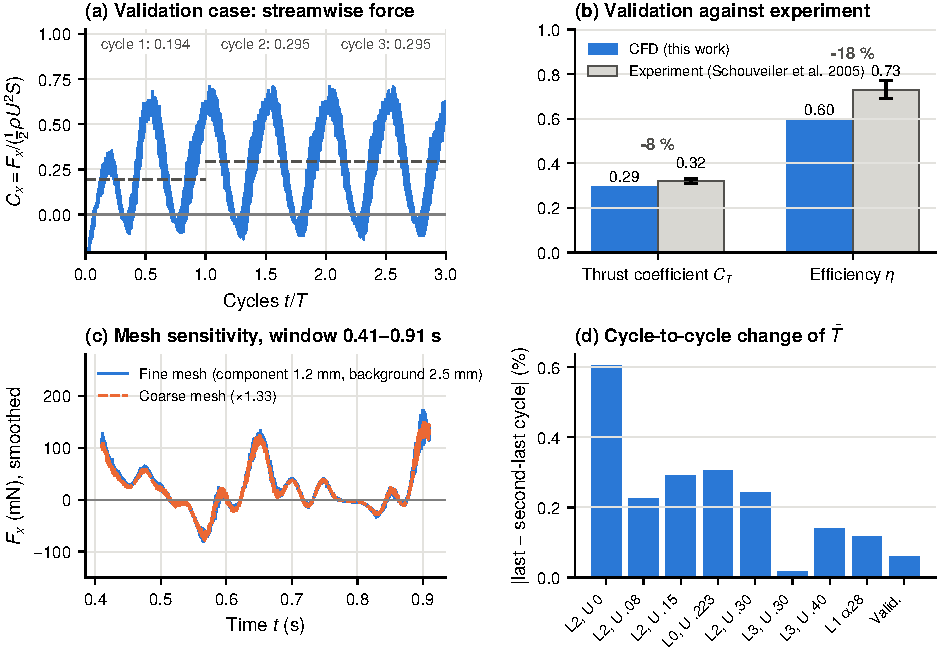
\includegraphics[width=\textwidth]{fig_verification}
  \caption[验证与确认]{单腿CFD的验证（verification）与确认（validation）。(a)确认算例：流向力系数及各周期平均值（虚线）。
    (b)推力系数和效率与Schouveiler等人\cite{Schouveiler2005}实验结果的对比。
    (c)尾鳍L0在细网格和粗网格上于共同时间窗口内的结果。
    (d)所有尾鳍算例及确认算例最后一个周期与倒数第二个周期之间平均推力的变化。}
  \label{fig:verification}
\end{figure}

\section{网格敏感性}
\label{sec:ver-mesh}

参考尾鳍算例L0在一套所有网格尺寸均乘以$r=1.33$的网格上重新计算（部件网格\SI{1.6}{\milli\metre}，背景网格\SI{3.3}{\milli\metre}）。
粗网格计算在$t=\SI{0.91}{\second}$时停止，因此两次计算在共同窗口$t=\SIrange{0.41}{0.91}{\second}$内进行比较。
两者的力时程在形状上几乎相同（\cref{fig:verification}c）。
粗网格得到的推力低7.3\,\%（\SI{19.75}{}对比\SI{21.30}{\milli\newton}），功率低3.9\,\%，效率低3.4\,\%。

仅有两套网格时无法计算收敛阶。假设为二阶收敛（$p=2$），并取安全系数$F_s=1.25$ \cite{Roache1994}，
则细网格上推力的网格收敛指数（grid convergence index，GCI）为
\begin{equation}
  \mathrm{GCI} = F_s\,\frac{|\varepsilon|}{r^p-1} = 1.25\times\frac{0.073}{1.33^2-1} \approx 12\,\%.
  \label{eq:gci}
\end{equation}
因此，尾鳍推力的离散不确定度取约$\pm12$\,\%，功率和效率的离散不确定度取约$\pm6$\,\%。
由于粗网格给出的推力较低，细网格的结果更可能略微偏低而非偏高。

\section{时间收敛性}
\label{sec:ver-time}

对于每个尾鳍算例，最后一个周期的平均推力与倒数第二个周期相差至多0.61\,\%（$\U=0$时的L2），
其余所有算例至多相差0.31\,\%（\cref{fig:verification}d）。确认算例相差不到0.1\,\%。
因此，在半周期启动之后对最后两个周期取平均已经足够；周期性状态在第一个完整周期内即已达到。
折扇桨算例在其第三个周期内进行评估。对于\SI{0.08}{\metre\per\second}下的机器人步态，第2和第3周期分别给出\SI{7.3}{}和\SI{5.2}{\milli\newton}；
该算例推力较小，其不确定度相应较大。

\section{对阻力型算例的影响}
\label{sec:ver-drag}

未对折扇桨单独进行网格研究，且其网格比尾鳍网格粗（\cref{tab:meshes}）。以下三点论据可界定其对结论的影响。
\begin{enumerate}
  \item \emph{流动物理。}桨是一块以板面正对运动方向运动、具有锐利边缘的薄板。其分离线固定在边缘上，
        而尾鳍的推力依赖于前缘涡（leading-edge vortex）和前缘吸力，二者对分辨率更为敏感。
        尾鳍的$\pm12$\,\%对桨而言是一个合理的上界。
  \item \emph{低速。}在\SI{0.15}{\metre\per\second}及以下，优化后的桨所产生的推力是尾鳍的1.6--2.0倍。
        $\pm12$\,\%的误差不会改变这一排序。
  \item \emph{交叉点。}在交叉点（crossover）附近，推力以约\SI{-110}{}（尾鳍）和\SI{-340}{\milli\newton\second\per\metre}（桨）的斜率下降。
        桨推力$\pm12$\,\%的误差（约\SI{2.5}{\milli\newton}）使交叉点移动约\SI{0.01}{\metre\per\second}；
        两侧方向相反的$\pm12$\,\%误差使其移动约\SI{0.02}{\metre\per\second}。
        附加质量修正的不确定度（见\cref{sec:cfd-composite}）带来的额外影响小于\SI{0.01}{\metre\per\second}。
\end{enumerate}
尽管如此，较粗的桨网格仍是一项局限性（limitation），列于\cref{sec:disc-limits}。

\section{实时求解器的交叉检验}
\label{sec:ver-flare}
\label{sec:res-flare}

Flare Live（\cref{sec:cfd-flare}）能够实时仿真整机，但所用格子（lattice）的间距为\SIrange{2}{3}{\milli\metre}。在使用其任何结果之前，先以CFD为基准检验其尾鳍力。在拖曳仿真（tow run）中，尾鳍执行与CFD完全相同的L0运动。其攻角一致（\SI{0.223}{\metre\per\second}时$\alpha_{75}=\SI{19.7}{\degree}$，对比\SI{19.9}{\degree}），但推力并不一致（\cref{fig:flare-fin}）。在\SI{3}{\milli\metre}格子上，Flare Live在\SIlist{0;0.1;0.223}{\metre\per\second}下分别给出\SI{20.0}{}、\SI{8.5}{}和\SI{-0.1}{\milli\newton}，而CFD中为\SI{45.5}{}、约\SI{34}{}（插值）和\SI{21.4}{\milli\newton}（\cref{tab:app-flare}）：分别为其44\,\%、25\,\%和几乎为零。在全部三个航速下，差额均约为\SIrange{21}{26}{\milli\newton}，与升力型推力本身处于同一量级。

保持在零位、不拍动的尾鳍在\SI{0.223}{\metre\per\second}时的阻力为\SI{12.6}{\milli\newton}。在其\SI{-25}{\degree}的入射角下，这相当于基于平面面积约0.45的阻力系数，对失速平板而言属于正常值。拍动相对于不拍动的推力增量为\SI{12.5}{\milli\newton}，仍远低于CFD推力。

在\SI{2}{\milli\metre}格子上，\SI{0.223}{\metre\per\second}时的尾鳍推力升至\SI{4.1}{\milli\newton}（为CFD的19\,\%），不拍动时的阻力几乎不变（\SI{11.6}{\milli\newton}）。该结果尚未收敛，基于两套格子的理查森外推（Richardson extrapolation）也仅给出约\SIrange{8}{12}{\milli\newton}，这表明这两套格子远未进入渐近区间。原因在于分辨率：\SI{34}{\milli\metre}的弦长在\SI{3}{\milli\metre}格子上仅跨越11个单元，在\SI{2}{\milli\metre}格子上为17个，而在$\mathit{Re}\approx7600$时边界层厚度约为\SI{0.4}{\milli\metre}。驱动升力型推力的吸力作用于前缘，而前缘未能被解析。要解析前缘，需要\SI{1}{\milli\metre}或更细的格子，计算代价将成倍增加，这违背了实时求解器的初衷。

\begin{figure}[t]
  \centering
  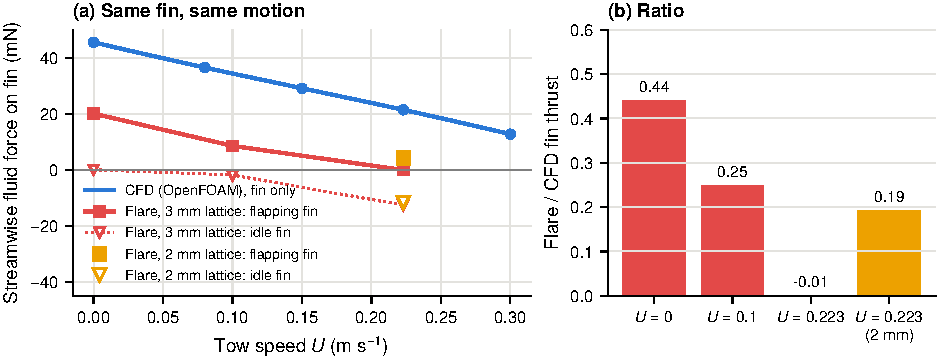
\includegraphics[width=\textwidth]{fig_flare_fin}
  \caption[Flare Live与CFD的对比]{对于相同的尾鳍和运动，Flare Live与CFD中的尾鳍力。(a) 拍动与不拍动时流向力随拖曳速度的变化。(b) Flare推力与CFD推力之比。}
  \label{fig:flare-fin}
\end{figure}

因此，Flare Live仅用于提供尾鳍的参考运动以及自由游动机器人的定性趋势（汇总于\cref{app:flare-trends}）；所有定量结论均以CFD为依据。

\section{小结}
\label{sec:ver-summary}

\Cref{tab:uncertainty}汇总了本章的各项检验。

\begin{table}[H]
  \centering
  \caption[不确定度汇总]{验证与确认汇总。}
  \label{tab:uncertainty}
  \small
  \begin{tabularx}{\textwidth}{@{}l>{\raggedright\arraybackslash}X@{}}
    \toprule
    检验项 & 结果 \\
    \midrule
    确认（翼型实验） & $C_T$ $-8$\,\%，$\etaF$ $-18$\,\%；偏差主要来自自由翼尖和层流模型 \\
    网格敏感性（尾鳍） & 在粗化$\times1.33$的网格上$\Tm$ $-7.3$\,\%，GCI $\approx\pm12$\,\% \\
    时间收敛性 & 尾鳍：最后两个周期相差$\le0.61$\,\%；机器人步态（\SI{0.08}{\metre\per\second}）：7.3对\SI{5.2}{\milli\newton} \\
    阻力型网格 & 未研究；排序不敏感，交叉点变化在$\pm\SI{0.02}{\metre\per\second}$以内 \\
    实时求解器（Flare Live） & 在2--3\,mm格子上尾鳍推力为CFD的0--44\,\%；仅用于趋势分析 \\
    \bottomrule
  \end{tabularx}
\end{table}

单腿CFD能够很好地再现拍动翼的推力，但低估了其效率。其数值不确定度以空间离散为主，推力的不确定度约为$\pm12$\,\%。
因此，在\cref{ch:results}中，推进器之间小于约15\,\%的差异不被视为显著。

\chapter{结果}
\label{ch:results}

本章报告单腿CFD结果，以及由此对整机得出的结论。本章首先设计阻力型划水动作（drag-type stroke）（\cref{sec:res-drag}）并表征尾鳍（fluke）的性能（\cref{sec:res-lift}），随后在不同航速下比较二者（\cref{sec:res-compare}），通过使尾鳍俯仰角随航速调度来改进尾鳍（\cref{sec:res-l3}），预测机器人的巡航速度（cruising speed）（\cref{sec:res-selfprop}），最后将其与首次硬件测试进行比较（\cref{sec:res-hw}）。除非另有说明，所有力和功率均为单腿值，且仅针对推进器本身。

\section{阻力型划水动作的设计}
\label{sec:res-drag}

阻力型划水动作在$\U=0$条件下按每次只改变一个因素的方式进行优化。\cref{sec:fund-paddle}中的准稳态模型（quasi-steady model）作为代理模型（surrogate）提出每一步改动，再由CFD对其进行评估；随后，在两态合成（two-state composite）结果上针对两个切换相位对折叠时机进行了优化。\Cref{tab:drag-design}列出了各个步骤。

\begin{table}[t]
  \centering
  \caption[阻力型划水动作的设计步骤]{$\U=0$时阻力型划水动作的设计步骤。每一步均在前一步的基础上改变一个方面。$\Tm$为两态合成的周期平均推力。除最后一步外，所有步骤均在髋关节运动的换向点切换扇面状态，在该处附加质量修正式\eqref{eq:addedmass}于$\U=0$时为零；对最后一步则给出了该修正的范围。}
  \label{tab:drag-design}
  \small
  \begin{tabularx}{\textwidth}{@{}l>{\raggedright\arraybackslash}Xcccc@{}}
    \toprule
    划水动作 & 改动 & $T$ (s) & DUTY & $\Tm$ (mN) & $\Pm$ (mW) \\
    \midrule
    机器人步态 & 基准；收拢宽度30\,mm，\SI{60}{\degree}正弦摆动 & 1.25 & 0.50 & 23.4 & 6.7 \\
    V1 & 周期更短，推力更大 & 0.89 & 0.49 & 51.2 & -- \\
    V2 & 划水冲程更短 & -- & 0.35 & 34.2 & -- \\
    V3 & 摆动以竖直方向为中心（\SIrange{120}{70}{\degree}），慢速卷收 & 0.81 & 0.45 & 49.3 & 16.2 \\
    V3c12 & 扇收拢至12\,mm而非30\,mm & 0.81 & 0.45 & 56.7 & 13.7 \\
    V3c06 & 收拢并顺桨，迎流宽度5.6\,mm & 0.81 & 0.45 & 58.6 & 13.1 \\
    V3trap & V3c12采用梯形速度规律（\SI{45}{\milli\second}斜坡） & 0.72 & 0.382 & 75.0 & 20.8 \\
    V3trap，调整时机 & 在减速开始时合扇，$\tau_c=0.33$ & 0.72 & 0.382 & \textbf{73--83} & 21.6 \\
    \bottomrule
  \end{tabularx}
\end{table}

\paragraph{划水方向。}使摆动以竖直方向为中心，可使桨几乎笔直地向后运动，且桨面垂直于运动方向。从V1到V3，划水冲程（power stroke）合力相对于游动方向的倾角由\SI{19.5}{\degree}降至\SI{7.9}{\degree}，平均竖直力与平均水平力之比由0.52降至0.28。V2表明，若回程（recovery）无法相应地变得更省力，仅缩短划水冲程会损失推力。

\paragraph{收拢宽度。}将扇收拢至\SI{12}{\milli\metre}而非\SI{30}{\milli\metre}，使回程阻力由\SI{-10.7}{}减小至\SI{-3.2}{\milli\newton}，并使平均推力提高15\,\%。有效面积比（effective area ratio）$a$定义为仅合扇算例与仅开扇算例的平均力之比，其值由0.48降至0.11。取$a=0.11$，由式\eqref{eq:duty-opt}可得$x^*=2.2$和$\mathrm{DUTY}^*=0.69$：回程应远快于划水冲程，而舵机转速不允许这样做。因此，最终冲程的DUTY为0.382，它并非由式\eqref{eq:duty-opt}得出，而是在舵机所允许的关节速度范围内（\cref{tab:actuators}）通过CFD优化求得。将收拢后的扇进一步顺桨（feathering）至\SI{5.6}{\milli\metre}的迎流宽度，仅带来3\,\%的提升：回程阻力与宽度成正比，但在\SI{12}{\milli\metre}时它仅约为平均推力的6\,\%。因此，顺桨机构并不值得采用。

\paragraph{速度规律。}在峰值角速度和摆幅不变的条件下，将余弦型髋关节速度替换为带\SI{45}{\milli\second}斜坡的梯形速度规律（trapezoidal velocity law），使划水冲程冲量提高了18\,\%，与准稳态的$\int v^2\,\mathrm dt$所预测的一致；平均推力则提高了32\,\%，因为周期同时由\SI{0.81}{}缩短至\SI{0.72}{\second}。其代价是更高的髋关节峰值力矩（\SI{35.6}{}而非\SI{19.3}{\milli\newton\metre}，$\times1.84$）、更高的峰值力以及多52\,\%的功率；单位功率推力由\SI{4.1}{}降至\SI{3.6}{\newton\per\watt}。CFD中划水冲程的有效法向力系数为准稳态值的2--3倍，且在冲程开始时最高，这与对突然起动平板的预期相符\cite{Kim2011}；该系数在两种速度规律下相同。

\paragraph{折叠时机。}两态合成方法（\cref{sec:cfd-composite}）允许在仿真完成后对折叠时机进行扫描。不加修正时，最佳组合为$\tau_c=0.33$、$\tau_o=-0.06$，对应\SI{87.2}{\milli\newton}。然而，在换向之前开扇所带来的增益正是\cref{sec:cfd-composite}所述的假象（artefact），因此扇在换向时打开，即$\tau_o=0$。提前合扇，即在划水冲程减速开始时合扇（$\tau_c=0.33$，0.86\,DUTY），可使未经修正的合成结果由\SI{75.0}{}提高至\SI{82.7}{\milli\newton}：处于减速中的张开扇面不再被其自身带动起来的水向后拖拽。这部分水能否保持其动量，取决于其中有多少以停止涡（stopping vortex）的形式脱落，因此附加质量修正（added-mass correction）式\eqref{eq:addedmass}给出了\SIrange{73}{83}{\milli\newton}的范围。因此在静止状态下，提前合扇的收益介于$-2$与$+8$\,mN之间。在有前进速度时，提前合扇从不更差，且最多可高出\SI{10}{\milli\newton}，因为在$\tau\approx0.33$之后，桨向后运动的速度低于迎面来流，张开的扇只会产生阻力；在\SI{0.223}{\metre\per\second}时，于$\tau_c=0.33$合扇得到\SIrange{24}{26}{\milli\newton}，而在换向点合扇则为\SIrange{14}{26}{\milli\newton}。最终的划水动作在本论文后文中称为V3trap（\cref{fig:composite,fig:kinematics}a），它在静止时每条腿产生\SIrange{73}{83}{\milli\newton}，为机器人当前步态的3.1--3.5倍，功率为\SI{21.6}{\milli\watt}，单位功率推力为\SIrange{3.4}{3.8}{\newton\per\watt}。这些规律与在甲壳类动物和蹼足推进器中发现的规律一致：在划水冲程开始时完全张开、提前收拢、并使状态转换保持短暂\cite{Santos2026,Lin2024}。

\section{采用固定俯仰规律的升力型尾鳍}
\label{sec:res-lift}

\Cref{tab:lift}列出了尾鳍采用L0运动时在五个航速下的结果。静止时来流完全沿竖直方向，尾鳍处于失速状态（$\alpha_{75}=\SI{73}{\degree}$），其作用相当于一块小桨；它以\SI{18.1}{\milli\watt}的功率产生\SI{45.5}{\milli\newton}的推力，约为采用折扇桨（fan paddle）的机器人步态推力的两倍。随着航速增加，来流角（inflow angle）和攻角（angle of attack）减小，推力几乎呈线性下降，在\SI{0.30}{\metre\per\second}时降至\SI{12.7}{\milli\newton}。输入功率保持在\SI{15.6}{}至\SI{18.1}{\milli\watt}之间。效率在\SI{0.223}{\metre\per\second}时升至最大值0.29，该航速正是L0的设计航速（基于销轴位移的$\mathit{St}\approx0.35$，$\alpha_{75}=\SI{19.9}{\degree}$）。在\SI{0.30}{\metre\per\second}时，冲程中段的攻角降至约\SI{10}{\degree}，效率降至0.245，并出现\SI{-29}{\milli\newton}的平均竖直力，其大小超过推力的两倍。

\begin{table}[t]
  \centering
  \caption[采用L0运动的尾鳍]{不同航速下采用L0运动（固定俯仰规律，fixed pitch schedule）的尾鳍。$\mathit{St}$基于\SI{39.2}{\milli\metre}的销轴峰峰位移计算。}
  \label{tab:lift}
  \small
  \begin{tabular}{@{}lccccc@{}}
    \toprule
    $\U$ (\si{\metre\per\second}) & 0 & 0.08 & 0.15 & 0.223 & 0.30 \\
    \midrule
    $\Tm$ (mN) & 45.5 & 36.5 & 29.1 & 21.4 & 12.7 \\
    $\Pm$ (mW) & 18.1 & 17.1 & 16.6 & 16.3 & 15.6 \\
    $\etaF$ & -- & 0.171 & 0.263 & 0.293 & 0.245 \\
    $\Tm/\Pm$ (\si{\newton\per\watt}) & 2.51 & 2.13 & 1.75 & 1.31 & 0.81 \\
    $\mathit{St}$ & -- & 0.98 & 0.52 & 0.35 & 0.26 \\
    \bottomrule
  \end{tabular}
\end{table}

\SI{0.223}{\metre\per\second}时的尾流（\cref{fig:wake}）呈现出产生推力的拍动翼所应有的形态：每半个冲程从尾缘脱落一个符号交替的涡，这些涡构成向下游对流的反卡门涡街（reverse von K\'arm\'an street）。

\begin{figure}[t]
  \centering
  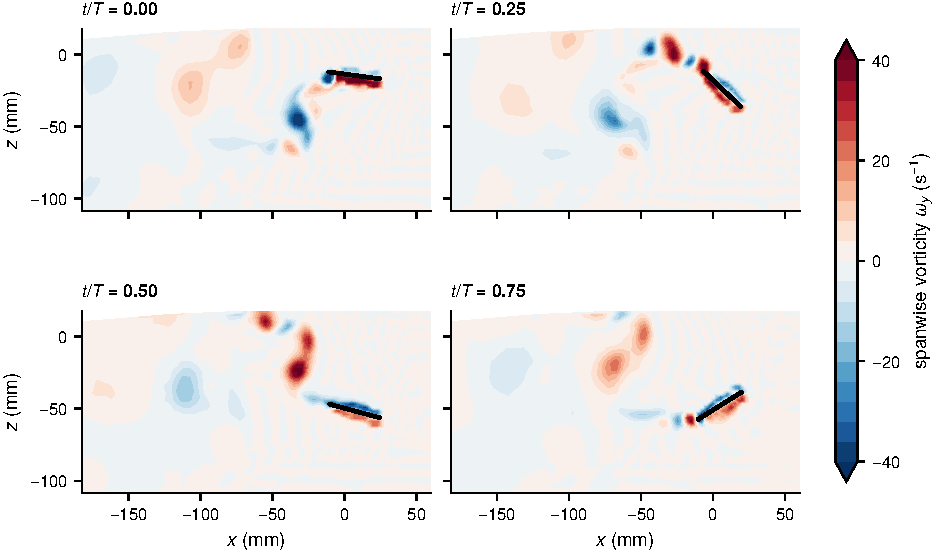
\includegraphics[width=\textwidth]{fig_wake}
  \caption[尾鳍的尾流]{尾鳍展长中面内的展向涡量（L0，$\U=\SI{0.223}{\metre\per\second}$），取第三个周期中的四个相位，船体坐标系；相对于尾鳍，流动方向为从右向左。黑线：尾鳍弦线。}
  \label{fig:wake}
\end{figure}

在\SI{0.223}{\metre\per\second}下，按目标攻角\SI{10}{\degree}和\SI{28}{\degree}设计的另外两种俯仰规律产生的推力均高于L0，但效率较低（分别为0.20和0.24，\cref{tab:app-fluke}）；在该航速下的各算例中，$\alpha_{75}\approx\SI{20}{\degree}$时效率最高，这与拍动翼的高效区间一致\cite{Read2003}。

\section{不同航速下阻力型与升力型推进的对比}
\label{sec:res-compare}

\Cref{fig:thrust-speed}比较了各推进器从静止到\SI{0.40}{\metre\per\second}的推力、功率和效率；\cref{tab:compare}给出了具体数值。

\begin{figure}[t]
  \centering
  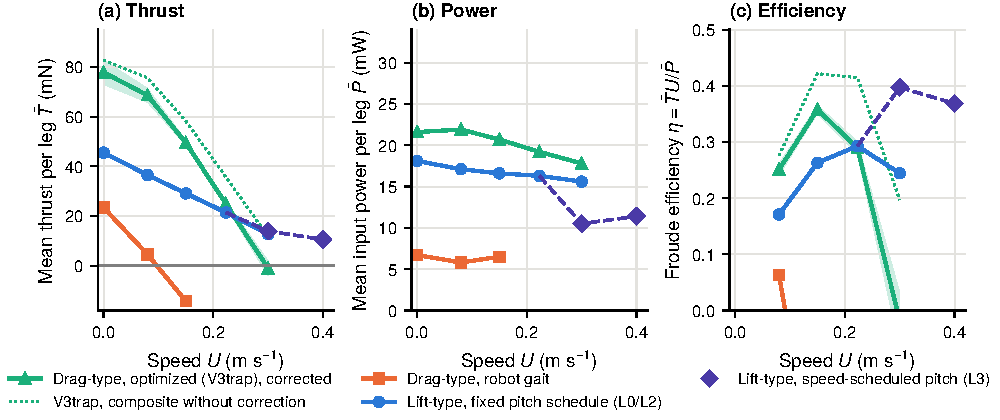
\includegraphics[width=\textwidth]{fig_thrust_speed}
  \caption[推力、功率和效率随航速的变化]{各推进器单腿的(a)推力、(b)输入功率和(c)弗劳德效率随航速的变化。阴影：桨合成结果的附加质量修正式\eqref{eq:addedmass}的范围；点线：未经修正的V3trap合成结果。}
  \label{fig:thrust-speed}
\end{figure}

\begin{table}[t]
  \centering
  \caption[不同航速下的推进器对比]{不同航速下的单腿推力$\Tm$ (mN) / 输入功率$\Pm$ (mW) / 弗劳德效率$\etaF$。桨的数值以范围形式计入附加质量修正式\eqref{eq:addedmass}；V3trap未经修正的合成结果为82.7、75.6、58.2、35.7和\SI{11.7}{\milli\newton}。}
  \label{tab:compare}
  \footnotesize
  \begin{tabular}{@{}ccccc@{}}
    \toprule
    $\U$ (\si{\metre\per\second}) & 桨，机器人步态 & 桨，V3trap & 尾鳍，固定（L0/L2） & 尾鳍，调度（L3） \\
    \midrule
    0     & 23.4 / 6.7 / --         & \textbf{73--83} / 21.6 / --                & 45.5 / 18.1 / --      & -- \\
    0.08  & 4--5 / 5.8 / 0.05--0.07 & \textbf{66--71} / 21.9 / 0.24--0.26        & 36.5 / 17.1 / 0.17    & -- \\
    0.15  & $<0$ / 6.5 / --         & \textbf{48--50} / 20.7 / \textbf{0.35--0.37} & 29.1 / 16.6 / 0.26  & -- \\
    0.223 & --                      & 24--26 / 19.2 / 0.28--0.30               & 21.4 / 16.3 / 0.29    & -- \\
    0.30  & --                      & $-4$--2 / 17.8 / $\approx0$                & 12.7 / 15.6 / 0.24    & \textbf{13.9} / 10.5 / \textbf{0.40} \\
    0.40  & --                      & --                                       & --                    & 10.5 / 11.4 / 0.37 \\
    \bottomrule
  \end{tabular}
\end{table}

\paragraph{低航速。}在约\SI{0.15}{\metre\per\second}以下，优化后的桨明显更优。其推力为尾鳍的1.6--2.0倍，功率高19--28\,\%；在\SI{0.15}{\metre\per\second}时其效率达到0.35--0.37，高于尾鳍的最大值0.29。按单位面积计，静止时二者没有差别：桨为\SIrange{3.9}{4.5}{}，尾鳍为\SI{4.1}{\milli\newton\per\square\centi\metre}。在\SI{0.223}{\metre\per\second}时，尾鳍的单位面积推力已更高（\SI{1.9}{}对\SIrange{1.3}{1.4}{\milli\newton\per\square\centi\metre}）。相比之下，机器人步态的推力几乎随即丧失：在\SI{0.08}{\metre\per\second}时仅剩\SIrange{4}{5}{\milli\newton}，在\SI{0.15}{\metre\per\second}时净力已表现为阻力。

\paragraph{桨的航速上限。}桨的推力随航速急剧下降，并在约\SI{0.30}{\metre\per\second}时消失。将其分解为划水冲程和回程两部分（\cref{fig:drag-split}，数值见\cref{tab:app-split}）即可看出原因。V3trap的划水冲程推力下降了42\,\%，由\SI{88.0}{}降至\SI{50.9}{\milli\newton}，这是因为划水冲程中的相对速度减小。然而，回程阻力增长了七倍以上，由\SI{-5.3}{}增至\SI{-39.1}{\milli\newton}，因为收拢的桨和杆件此时迎着来流向前运动。在有航速时，开扇还会在每个周期损失动量$\Delta m_a\U$，在\SIrange{0.223}{0.30}{\metre\per\second}下相当于\SIrange{12}{16}{\milli\newton}。在\SI{0.30}{\metre\per\second}时，回程与开扇共同耗尽了全部划水冲程推力。对于机器人步态，由于其收拢后的扇更宽、划水动作更慢，回程阻力在约\SI{0.1}{\metre\per\second}时便已超过划水冲程推力。因此，该腿上阻力型桨的航速上限取决于桨在划水冲程之外必须完成的动作，而非桨在划水冲程中的速度。

\begin{figure}[t]
  \centering
  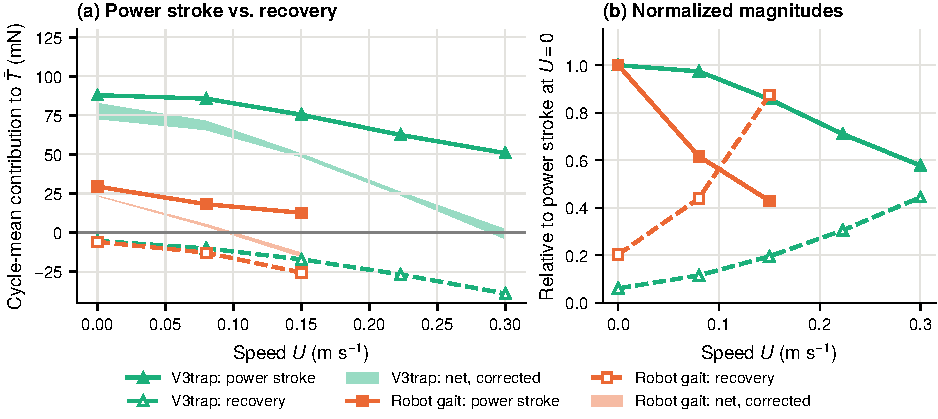
\includegraphics[width=\textwidth]{fig_drag_split}
  \caption[桨的划水冲程与回程]{划水冲程与回程对折扇桨平均推力的贡献。(a) V3trap和机器人步态的绝对值；阴影：计入附加质量修正式\eqref{eq:addedmass}后的净推力。(b) 相对于$\U=0$时划水冲程推力的幅值。}
  \label{fig:drag-split}
\end{figure}

\paragraph{交叉点。}尾鳍的推力下降较慢，因为它既不需要逆流回程，也不改变自身形状：其在\SI{0.30}{\metre\per\second}时的推力为静止时的28\,\%，而桨的推力已接近零。对曲线进行插值可知，尾鳍的推力在\SIrange{0.23}{0.24}{\metre\per\second}以上超过V3trap，其效率则在\SIrange{0.22}{0.23}{\metre\per\second}以上超过后者。这一结论对两种俯仰规律均成立，因为随航速调度的俯仰（speed-scheduled pitch）仅在\SIlist{0.30;0.40}{\metre\per\second}下进行了仿真，在更低航速下沿用L0的数据。计入\cref{sec:ver-drag}中的离散化不确定度后，推力的交叉点（crossover）位于$0.24\pm\SI{0.02}{\metre\per\second}$，效率的交叉点位于$0.22\pm\SI{0.02}{\metre\per\second}$。若不计附加质量修正，交叉点将分别位于\SI{0.295}{}和\SI{0.285}{\metre\per\second}；该修正使交叉点移动了约\SI{0.06}{\metre\per\second}，但并不改变其存在性。

\section{随航速调度的尾鳍俯仰}
\label{sec:res-l3}

采用固定的L0运动时，尾鳍的攻角随航速增加而减小，这解释了其效率在\SI{0.223}{\metre\per\second}以上的下降。随航速调度的俯仰式\eqref{eq:l3}使攻角得以恢复（\cref{fig:l3}）。在\SI{0.30}{\metre\per\second}时，它将俯仰幅值由约\SI{40}{\degree}减小至\SI{21.6}{\degree}，攻角相应增大：$\alpha_{75}$由\SI{13.7}{\degree}增至\SI{21.0}{\degree}（\cref{tab:l3,tab:app-fluke}）。

\begin{table}[t]
  \centering
  \caption[随航速调度的俯仰]{随航速调度的俯仰（L3）与固定L0运动（L2）的对比。$\bar F_z$：平均竖直力；$|M_h|$：绕销轴的铰链峰值力矩。}
  \label{tab:l3}
  \small
  \begin{tabular}{@{}lcccccc@{}}
    \toprule
    算例 & $\U$ (\si{\metre\per\second}) & $\Tm$ (mN) & $\Pm$ (mW) & $\etaF$ & $\bar F_z$ (mN) & $|M_h|$ (\si{\milli\newton\metre}) \\
    \midrule
    L2，固定俯仰 & 0.30 & 12.7 & 15.6 & 0.245 & $-29.4$ & 12.6 \\
    L3，调度俯仰 & 0.30 & \textbf{13.9} & \textbf{10.5} & \textbf{0.398} & $-0.9$ & 7.4 \\
    L3，调度俯仰 & 0.40 & 10.5 & \textbf{11.4} & \textbf{0.368} & $-0.9$ & 7.3 \\
    \bottomrule
  \end{tabular}
\end{table}

在\SI{0.30}{\metre\per\second}时，调度俯仰使推力提高9\,\%、功率降低33\,\%，并使效率由0.245提高至0.40，而桨在该航速下几乎不产生推力。它还消除了平均竖直力（由$-29$降至$\SI{-1}{\milli\newton}$），使铰链峰值力矩降低40\,\%，并使力的时间历程更加平缓：流向力的峰峰值由约\SI{600}{}降至\SI{190}{\milli\newton}。在\SI{0.40}{\metre\per\second}时，效率为0.37。在三个设计航速下，尾鳍效率分别为0.29（L0，0.223）、0.40（L3，0.30）和0.37（L3，0.40），最大值出现在\SI{0.30}{\metre\per\second}附近。在该航速下，基于销轴位移的斯特劳哈尔数（Strouhal number）为0.26，处于动物高效巡航的0.2--0.4范围之内，且接近齿鲸类的实测平均值\cite{Taylor2003,Rohr2004}；若基于尾缘位移计算，则该值略高。该调度规律无需任何流场信息，只需$\dot h_\text{max}$和$\U$。在硬件上，它对应于随航速减小的俯仰幅值；被动弹簧能在多大程度上实现这一规律，将在\cref{sec:disc-limits-prop}中讨论。

\begin{figure}[t]
  \centering
  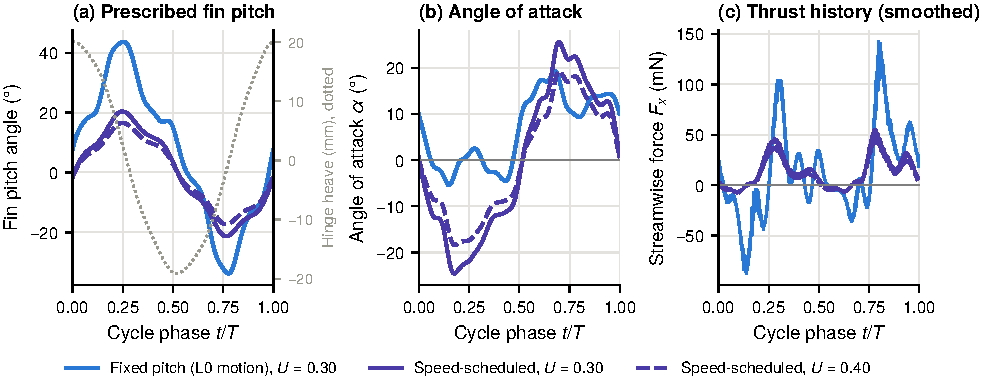
\includegraphics[width=\textwidth]{fig_l3}
  \caption[随航速调度的俯仰]{固定L0运动与随航速调度的俯仰的对比。(a) 给定的尾鳍俯仰角（铰链沉浮以点线表示，右轴）。(b) 由此得到的攻角。(c) 经平滑处理的流向力。}
  \label{fig:l3}
\end{figure}

\section{自航估计}
\label{sec:res-selfprop}

\paragraph{阻力。}三条阻力曲线界定了不含推进器的机器人所受阻力（resistance）的范围（\cref{fig:selfprop}a）：
\begin{itemize}
  \item $D_\text{low}=\SI{10.8}{\milli\newton}\,(\U/\SI{0.2}{\metre\per\second})^{1.72}$：裸船体，来自在\SIlist{0.1;0.2}{\metre\per\second}下单独对船体进行的两相CFD；
  \item $D_\text{mid}=D_\text{low}+\SI{15.2}{\milli\newton}\,(\U/\SI{0.2}{\metre\per\second})^2$：船体加上水下连杆，在\SI{0.2}{\metre\per\second}时约为\SI{26}{\milli\newton}；连杆项相当于$C_DA\approx\SI{7.6}{\square\centi\metre}$，是工程估计值而非测量值；这是最佳估计；
  \item $D_\text{up}=\SI{77.6}{\milli\newton}\,(\U/\SI{0.2}{\metre\per\second})^2$：静止且折扇桨张开状态下的整机，来自CFD；它计入了桨自身的阻力，而该阻力已包含在$\Tm$中，因此是一个上界。
\end{itemize}
推力曲线采用单调三次样条（monotone cubic splines）插值，并在最后一个CFD数据点之外作线性外推。

\begin{figure}[t]
  \centering
  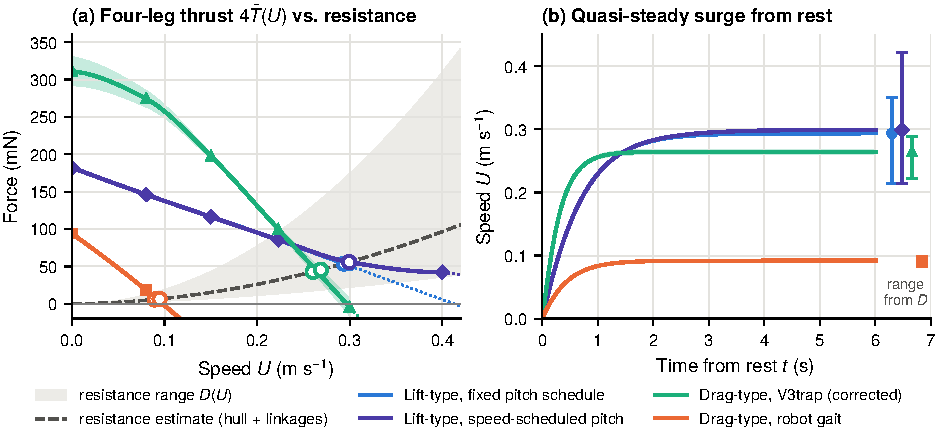
\includegraphics[width=\textwidth]{fig_selfprop}
  \caption[自航估计]{自航估计。(a) 四腿推力与阻力范围的对比；圆圈标出$D_\text{mid}$下的巡航速度；阴影：桨的附加质量修正范围。点线：线性外推。在\SI{0.30}{\metre\per\second}以下未对随航速调度的俯仰进行仿真，其曲线采用固定俯仰的数据。(b) $D_\text{mid}$下从静止开始的准稳态加速过程；右侧竖条给出了从$D_\text{up}$到$D_\text{low}$的巡航速度范围。}
  \label{fig:selfprop}
\end{figure}

\begin{table}[t]
  \centering
  \caption[预测的巡航速度]{$D_\text{mid}$下预测的巡航速度和四腿输入功率，以及从$D_\text{up}$到$D_\text{low}$的范围。桨的数值以附加质量修正的范围形式给出。$^*$：超出CFD数据范围的外推值。$t_{90}$：从静止达到巡航速度的90\,\%所需的时间。}
  \label{tab:selfprop}
  \small
  \begin{tabular}{@{}lccccc@{}}
    \toprule
    推进器 & $\U_c$ (\si{\metre\per\second}) & 范围 (\si{\metre\per\second}) & $4\Pm$ (mW) & $4\Pm/\U_c$ (\si{\joule\per\metre}) & $t_{90}$ (s) \\
    \midrule
    阻力型，机器人步态 & 0.089--0.095 & 0.082--0.098 & 23.3 & 0.25--0.26 & 0.94--0.99 \\
    阻力型，V3trap & 0.260--0.269 & 0.223--0.289 & 73--74 & 0.27--0.28 & 0.67--0.69 \\
    升力型，固定俯仰 & 0.294 & 0.214--0.350$^*$ & 62.7 & 0.21 & 1.46 \\
    升力型，调度俯仰 & \textbf{0.299} & 0.214--0.422$^*$ & \textbf{42.0} & \textbf{0.14} & 1.57 \\
    \bottomrule
  \end{tabular}
\end{table}

\paragraph{巡航速度。}在最佳估计阻力下，尾鳍推动机器人以\SI{0.30}{\metre\per\second}（即每秒1.3倍船体长度）的速度航行，优化后的桨则为\SIrange{0.26}{0.27}{\metre\per\second}（\cref{tab:selfprop}）。两个工作点均略高于交叉点，处于尾鳍更强的一侧，但距交叉点很近，因此速度差异很小。功率则差异明显：随航速调度俯仰的尾鳍需要\SI{42}{\milli\watt}，比固定俯仰的尾鳍（\SI{63}{\milli\watt}）低33\,\%，比桨（\SI{73}{\milli\watt}）低43\,\%，而桨的速度还更慢。机器人当前步态仅能达到约\SI{0.09}{\metre\per\second}。由于阻力存在不确定性，这些范围较宽，而哪种推进器更快取决于阻力曲线与推力曲线的交点位置。在高阻力$D_\text{up}$下，工作点移至交叉点以下，桨略快（\SIrange{0.22}{0.23}{}对\SI{0.21}{\metre\per\second}）；在低阻力$D_\text{low}$下，工作点进一步移至交叉点以上，尾鳍明显更快（\SIrange{0.35}{0.42}{\metre\per\second}，外推值，对\SIrange{0.28}{0.29}{\metre\per\second}）。

\paragraph{加速。}从静止开始的加速过程按实测质量\SI{0.419}{\kilo\gram}外加10\,\%的附加质量进行积分；质量只影响时间尺度，而不影响巡航速度。桨使机器人加速更快：它在\SI{0.68}{\second}后达到其巡航速度的90\,\%，尾鳍则需\SIrange{1.46}{1.57}{\second}（\cref{fig:selfprop}b）。这反映了桨在低航速下更高的推力，并与“划桨式附肢利于加速、拍动式附肢利于巡航”的观察结果相符\cite{Walker2000}。

\section{首次硬件测试}
\label{sec:res-hw}

对装配尾鳍的机器人（\cref{sec:plat-hw}）在一个\SI{1}{\metre}长的水池中进行了计时：机器人从静止起步，起步时尾部贴着一端池壁，船头撞到另一端池壁时停止计时，行程为\SI{0.738}{\metre}（水池长度减去船体总长\SI{262}{\milli\metre}）。冲程频率在固件中分别设为\SI{2}{}和\SI{4}{\hertz}，每个设定值各手动计时一次。同样的过程也用\cref{fig:selfprop}b的准定常模型进行了仿真，采用L0在\SI{2}{\hertz}下的推力和实测质量（\cref{tab:hw}）。

\begin{table}[htb]
  \centering
  \caption[首次硬件测试]{首次硬件测试：从静止起步游过\SI{0.738}{\metre}所用的时间和平均速度。频率为固件中的设定值。模型：L0在\SI{2}{\hertz}下的推力，配合\cref{sec:res-selfprop}中的三条阻力曲线。}
  \label{tab:hw}
  \small
  \begin{tabular}{@{}lccc@{}}
    \toprule
    & 设定频率 (Hz) & 时间 (s) & 平均速度 (\si{\metre\per\second}) \\
    \midrule
    硬件 & 2 & 5.2 & 0.142 \\
    硬件 & 4 & 2.8 & 0.264 \\
    模型，$D_\text{low}$ / $D_\text{mid}$ / $D_\text{up}$ & 2 & 2.9 / 3.2 / 3.9 & 0.25 / 0.23 / 0.19 \\
    \bottomrule
  \end{tabular}
\end{table}

\paragraph{推力。}在\SI{2}{\hertz}下，冲程与L0接近，取$D_\text{mid}$至$D_\text{up}$时，硬件所用时间是预测值的1.3至1.6倍（取$D_\text{low}$时为1.8倍，但$D_\text{low}$不适用于硬件）。仅凭阻力无法解释这一差异：若采用CFD推力，则需要在\SI{0.2}{\metre\per\second}时有\SI{205}{\milli\newton}的阻力，为$D_\text{up}$的2.6倍。这相当于$C_DA\approx\SI{103}{\square\centi\metre}$，按船体\SI{24}{\square\centi\metre}的水下迎流面积（frontal area）计，$C_D\approx4$，远高于任何钝体。$D_\text{up}$本身已相当于$C_D\approx1.6$，即使船体以钝端在前运动，也是一个宽松的上界；而$D_\text{low}$对应尖端在前的裸船体，不适用于硬件。在$D_\text{mid}$与$D_\text{up}$之间，若推力取CFD值的27--47\,\%，即大约四分之一到一半，即可再现该测试，相应的\SI{2}{\hertz}稳态速度约为\SIrange{0.16}{0.20}{\metre\per\second}。其中一部分亏损来自冲程本身：分段线性轨迹的峰值沉浮速度比L0低约15\,\%（\cref{sec:plat-hw}），约损失10--20\,\%的推力。其余约两倍的差距有多种可能原因，这次测试无法将它们区分开：被动俯仰（passive pitch），其弹簧刚度未按L0的攻角验证过；尾鳍冲出水面处的通气（ventilation）；反装的船体；以及腿间相互作用。因此，\cref{tab:selfprop}中的自航速度是现有硬件的上限（upper bound）。

\paragraph{频率。}两次测试之比与推力水平无关。若阻力随$\U^2$增长，且在斯特劳哈尔数固定时推力与冲程速度的平方成正比，则从静止起步游过给定距离所需的时间与频率和幅值的乘积成反比。实测时间之比\SI{5.2}{}比\SI{2.8}{\second}，即1.86，接近舵机在\SI{4}{\hertz}下达到完整幅值时应有的2，尽管由固件轨迹估算的舵机峰值转速约为\SI{800}{\degree\per\second}，已接近其空载转速。更精确的结论无法给出：每次计时\SI{0.2}{\second}的误差就会使该比值在1.67至2.08之间变化；而且被动俯仰随频率变化，因为水动力矩随冲程速度的平方增长，而弹簧力矩不变。若按表面值取用，同样的缩放关系给出\SI{4}{\hertz}下约\SIrange{0.3}{0.4}{\metre\per\second}的稳态速度，高于\SI{2}{\hertz}下基于CFD的估计值，但水动力功率约为其六倍。

\chapter{讨论}
\label{ch:discussion}

\section{对假设的评估}
\label{sec:disc-hyp}

\paragraph{H1（降阶优化）}在模型范围内得到支持。只要模型中包含升力且未被压制，全部101个可行最优解都是升力推进的（lift-propelled）。H1不仅在模型之间得到检验，即升力推进步态（gait）所需功率为最佳纯阻力步态的二分之一到三分之一；也在同一模型内得到检验：以升力占比限值强制的阻力型划动需要四至十倍的功率，且达不到\SI{0.30}{\metre\per\second}，不过这第二个倍数仅基于3个可行划动。如下文所述，这一结论以一个未经标定的升力模型为前提。

\paragraph{H2（阻力与升力随速度的对比）}得到支持。正如预期，经过优化的桨（paddle）在低速下明显更强，其推力（thrust）随速度急剧下降，在\SI{0.30}{\metre\per\second}时降至约零；尾鳍（fluke）则保留了更大比例的推力，并在\SIrange{0.23}{0.24}{\metre\per\second}以上变得更强。桨的速度极限的成因已经明确：一是回程（recovery）阻力，它从静止到\SI{0.30}{\metre\per\second}增大到原来的七倍以上；二是在迎面来流中开扇所需的动量；与此同时，划水冲程（power stroke）推力的下降不到一半。效率的交叉点（crossover）略低于推力的交叉点，位于约\SI{0.22}{\metre\per\second}；在此以下，经过优化的桨比尾鳍更强，效率也更高，在\SI{0.15}{\metre\per\second}时达到$\etaF=0.35$--0.37。这与生物学中的图景不同：在动物中，升力型游动者在所有速度下都比划水者更高效\cite{Fish1996}；而对于配备折叠性能良好的桨的小型机器人腿，这一点仅在交叉点以上成立。H2的第二部分得到证实：调度尾鳍的俯仰角（pitch），使攻角（angle of attack）保持在\SI{20}{\degree}附近，可将\SI{0.30}{\metre\per\second}时的效率从0.24提高到0.40。

桨的效率超过了Fish针对划水动物所报告的约0.33的最大值\cite{Fish1984,Fish1996}。这两个数值不能直接比较：动物的数值是针对整个动物的估计值，而此处的$\etaF$是一个孤立推进器（propulsor）的水动力弗劳德效率（Froude efficiency），该推进器收拢后的扇面所产生的力仅约为张开扇面的九分之一（$a=0.11$，而麝鼠的面积比为0.445）。它也仍低于\SI{0.15}{\metre\per\second}时的准定常上限$\U/v_p\approx0.6$，其中扇面形心的平均划水冲程速度为$v_p\approx\SI{0.25}{\metre\per\second}$。

\paragraph{H3（整机）}基本得到支持。采用阻力（resistance）的最佳估计值时，尾鳍达到\SI{0.30}{\metre\per\second}，桨达到\SIrange{0.26}{0.27}{\metre\per\second}，因此两者速度相近但不相等；而随航速调度俯仰的尾鳍所需功率比桨低43\,\%（\SI{42}{}对\SI{73}{\milli\watt}）。不过，首次硬件测试比预测慢1.3至1.6倍（\cref{sec:res-hw}）。因此，预测速度是现有机器人的上限，而推进器之间的比较以CFD为依据。

\section{降阶模型与CFD为何在低速下存在差异}
\label{sec:disc-models}

降阶模型（reduced-order model）与CFD一致表明：阻力型划水（drag-based paddling）存在速度极限，而升力型拍动（lift-based flapping）在巡航速度（cruising speed）下占优。两者在低速下存在分歧：MuJoCo发现升力推进的步态在\SI{0.10}{\metre\per\second}时就已更为经济，差距约为二至四倍（在\SI{0.20}{\metre\per\second}时可达十倍），而CFD则发现经过优化的桨在约\SI{0.22}{\metre\per\second}以下效率更高。以下四点差异可以解释这一现象。
\begin{enumerate}
  \item \emph{升力模型偏乐观。}平板律$c_l\sin2\alpha$在产生升力时不含有限翼的诱导阻力和翼尖损失，而 toy\_quad 模型中脚蹼的展弦比（aspect ratio）仅为1.4。确认（validation）算例提示，即使在展弦比为6时，有限展长也很可能是高达18\,\%的效率亏损的原因之一，翼尖损失估计为10--20\,\%。该模型也不包含动态失速、环量建立的延迟以及脚蹼与其自身尾流的相互作用。
  \item \emph{对于起动中的桨，阻力模型偏悲观。}恒定的$C_D=2.2$忽略了起动涡（starting vortex）和附加质量（added mass）效应，而在CFD中，这些效应将桨划水冲程的有效力系数提高到其准定常值的2--3倍（\cref{sec:res-drag}）。
  \item \emph{阻力型冲程不同。}MuJoCo中的脚蹼只能通过转动来顺桨（feathering），既不能折叠（fold），也没有受控的折叠时机，并且仅限于式\eqref{eq:gait}的平滑谐波运动。由于斜着划过水的脚蹼会产生升力，升力模型中的阻力型划动实际上是被压制了升力的划动，而纯阻力模型中的大多数划水型划动在加入升力后都变为升力推进（\cref{sec:mj-liftshare}）。相比之下，CFD中的桨是专门的阻力装置：它以板面正对运动方向运动，在经过优化的相位下折叠至12\,mm，并采用梯形速度规律，上述每项特征各自可带来最多约30\,\%的推力提升。因此，MuJoCo比较的是升力型划动与被压制升力的脚蹼划动，而CFD比较的是尾鳍与经过优化的折叠桨。
  \item \emph{优化投入在两个方向上都不对称。}在MuJoCo中，升力步态针对给定所需速度下的功率进行了优化，而纯阻力前沿尚未收敛，升力模型内针对阻力型划动的带约束搜索在30次运行中也只有3次找到可行解。在CFD中，桨经过了多轮优化，而尾鳍运动L0取自另一个模型，之后仅对其俯仰幅值进行了随航速的调度。两者的面积也不同（\SI{18.5}{}对\SI{11.2}{\square\centi\metre}）。
\end{enumerate}
因此，降阶模型最好理解为关于\emph{机理}的论据，即优化器在条件允许时会利用哪种推进原理；而CFD则是关于\emph{量级}以及一种原理超越另一种原理时所处速度的论据。在两者存在分歧之处，以解析了流场且经过确认的CFD为准。以CFD为基准标定降阶模型的系数，尤其是带展弦比修正的$c_l$，将使两者协调一致，这也是顺理成章的下一步。

\section{对BODY2的启示}
\label{sec:disc-design}
\label{sec:disc-limits-prop}

\paragraph{建议。}对于在水面横渡开阔水域的任务，推荐BODY2采用俯仰角随航速减小的尾鳍作为推进器。在最佳估计阻力下，它比经过优化的桨V3trap略快，所需水动力功率（hydrodynamic power）低43\,\%，并且既不需要受控折叠，也不需要梯形速度规律。与机器人目前的配置相比，它使预测的巡航速度提高到约三倍；在硬件上一次未计时的对比中，尾鳍也明显比桨游得快（\cref{sec:plat-hw}）。在加速、低速定点保持或行走较为重要的场合，桨仍是更好的选择；此时需要一种收拢宽度（folded width）减小至约\SI{12}{\milli\metre}、并能在特定相位于\SIrange{45}{60}{\milli\second}内受控完成的折叠，而目前的拉线折叠机构无法做到这一点。这种分工，即划桨用于起步和低速、拍动用于巡航，正是在动物中发现的分工\cite{Walker2000,Fish1996}；一条能够从桨切换为尾鳍的腿（如Baines等人\cite{Baines2022}的可变形龟类肢体）将能够覆盖这两种工况。

\paragraph{尾鳍。}尾鳍在静止时的推力有限，因为它处于失速状态：没有前进速度时，拍动翼（foil）就相当于一个小桨。有航速时，其性能取决于能否使攻角保持在高效范围附近，而固定俯仰规律（fixed pitch schedule）做不到这一点。调度规律$\theta_0=\gamma_\text{max}/2$是一个能够实现这一点的单参数规则，同时还消除了不匹配的规律所产生的较大平均垂向力。在硬件上，俯仰是被动的：它由绕销轴（pin）的水动力力矩（使尾鳍转向来流方向）与板簧（leaf spring）之间的平衡决定。因此，被动尾鳍能够适应航速，但适应的比例并不符合要求。水动力力矩随相对速度的平方增长，而弹簧力矩则不然，因此比值$\theta/\gamma$随航速增大。线性弹簧只能在一个设计航速下满足$\theta_0=\gamma_\text{max}/2$；低于该航速时，尾鳍俯仰不足，攻角过大；高于该航速时，尾鳍与来流过度对齐，攻角降至高效范围以下。要在一段航速范围内实现匹配，需要渐进刚度弹簧、可调预紧力或主动俯仰执行器。硬件测试仅达到CFD推力的大约四分之一到一半（\cref{sec:res-hw}），这与被动俯仰未调至高效攻角相符，但不能排除其他原因。

\paragraph{等面积。}本文所用尾鳍的面积为桨的61\,\%。静止时两者的单位面积推力相同（\SIrange{3.9}{4.5}{}对\SI{4.1}{\milli\newton\per\square\centi\metre}），而在\SI{0.223}{\metre\per\second}时尾鳍已产生更大的单位面积推力（\SI{1.9}{}对\SIrange{1.3}{1.4}{\milli\newton\per\square\centi\metre}）。若推力系数和功率系数保持不变，一个与桨面积相同（\SI{18.5}{\square\centi\metre}）、按相同运动学运动的尾鳍，在静止时将产生约\SI{75}{\milli\newton}的推力，与桨相当，并且从约\SI{0.15}{\metre\per\second}起超过桨。其功率将按相同比例增长，静止时约为\SI{30}{\milli\watt}，因此效率交叉点不会移动。已为该机器人设计了一个具有此面积的月牙形尾鳍（展长\SI{86}{\milli\metre}，$\mathit{AR}\approx4$）；其较大的展弦比应能减小翼尖损失，但其较大的铰链力矩（在相同俯仰规律下约为A2的1.6倍）必须由俯仰弹簧或执行器承担。这是估算值，而非仿真结果。

\paragraph{执行器。}所有运动的水动力力矩与舵机（servo）相比都很小：其中最大的是梯形桨冲程绕髋（hip）关节的\SI{36}{\milli\newton\metre}，为PTK\,7465W堵转力矩（stall torque，\SIrange{0.44}{0.57}{\newton\metre}）的6--8\,\%。真正起作用的限制是关节速度以及切换折叠的能力（\cref{tab:actuators}）。L0的给定俯仰需要\SI{712}{\degree\per\second}，超过\SI{6}{\volt}时的空载转速（no-load speed，\SI{650}{\degree\per\second}），并接近\SI{8.4}{\volt}时的空载转速（\SI{860}{\degree\per\second}）；而\SI{0.30}{\metre\per\second}时随航速调度的俯仰（speed-scheduled pitch）仅需\SI{366}{\degree\per\second}。

\section{局限性}
\label{sec:disc-limits}

\begin{itemize}
  \item \emph{单腿。}CFD仅模拟一个推进器，不含连杆、船体（hull）和其他腿。腿间相互作用可使四条划水腿的推力高于单腿值的四倍\cite{Wang2025}，且这种作用在桨与尾鳍之间可能有所不同。自航（self-propulsion）平衡忽略了这一点。
  \item \emph{自由液面。}所有针对推进器的CFD均为带刚性盖（rigid lid）的单相计算。在硬件上和Flare Live中，尾鳍在冲程顶端会冲出水面约\SI{7}{\milli\metre}，而桨的回程路径也接近水面；通气和波浪均未建模。
  \item \emph{给定的俯仰与折叠。}尾鳍俯仰以刚性方式给定，而硬件上的尾鳍是被动的。扇面的折叠被建模为两个分别模拟的状态之间的瞬时切换。切换时附加质量的变化在一定界限内通过解析方法修正，所用附加质量由CFD辨识得到；张开状态算例自身的回程尾流对其划水冲程的影响未作修正，这使桨的结果略偏乐观。
  \item \emph{CFD精度。}流动按层流处理，这是$\mathit{Re}=4\times10^4$的确认算例中出现18\,\%效率亏损的原因之一；在尾鳍所处的较低雷诺数下，预计该影响较小。尾鳍推力约有$\pm12$\,\%的离散不确定性。桨的网格更粗，且未单独进行研究；\cref{sec:ver-drag}中已论证，结论对该量级的误差不敏感。
  \item \emph{功率。}此处的功率是推进器的水动力输入功率（input power）。舵机损耗、腿的惯性和连杆的阻力均未计入，因此推进器之间的功率比并不等于电池功率之比。
  \item \emph{推进器不对等。}桨的冲程比尾鳍运动优化得更充分，因此尾鳍的结果偏保守，对沉浮（heave）幅值、频率和俯仰进行系统优化很可能使交叉点移向更低速度。两种推进器还以不同频率运行（\SI{1.39}{}和\SI{2}{\hertz}），面积也不同；文中给出了单位面积推力和单位功率推力，但未进行等面积、等频率的比较。
  \item \emph{阻力。}船体阻力仅在一定界限内已知，巡航速度也相应存在不确定性。$D_\text{mid}$中的连杆项是工程估算值，而非测量值；此外，船体阻力是按尖端在前计算的，而硬件以钝端在前游动。
  \item \emph{降阶模型。}MuJoCo模型是一个尺寸相近的替代模型，并非BODY2，且其系数未经标定。其舵机模型（\SI{3}{\newton\metre}，\SI{400}{\degree\per\second}）比PTK\,7465W（\SIrange{0.44}{0.57}{\newton\metre}，\SIrange{650}{860}{\degree\per\second}）力矩更大、速度更慢。其搜索未完全收敛，模型内比较仅基于30次搜索（两个种子）中的3个可行阻力型划动，因此其功率倍数可能被高估。
  \item \emph{硬件。}硬件测试仅包括每个频率一次从静止起步的手动计时，船体反装，俯仰为被动，冲程幅值未测量。它表明自航估计是上限，但无法确定差异的原因。
\end{itemize}

\chapter{结论与展望}
\label{ch:conclusion}

\section{结论}

本文针对两栖四足机器人BODY2的腿部，比较了阻力型划水（drag-based paddling）与升力型拍动（lift-based flapping），所用方法包括基于降阶模型的步态优化（reduced-order gait optimization）和真实腿部的单腿CFD。\Cref{tab:key-findings}给出了对三个研究问题（research question）的回答。

\begin{table}[H]
  \centering
  \caption[主要结论]{对研究问题的回答。桨（paddle）：经过优化的折扇桨V3trap；尾鳍（fluke）：除另有说明外，指采用随航速调度俯仰L3的A2；功率均为水动力功率。}
  \label{tab:key-findings}
  \small
  \begin{tabularx}{\textwidth}{@{}>{\raggedright\arraybackslash}p{27mm}>{\raggedright\arraybackslash}p{40mm}>{\raggedright\arraybackslash}X@{}}
    \toprule
    问题 & 回答 & 关键数据 \\
    \midrule
    RQ1：优化器选择的机理（\cref{ch:mujoco}） &
      只要模型中包含升力，即选择升力 &
      只要升力未被压制，含升力模型的全部101个可行最优解都是升力推进的（lift-propelled）。在相同速度下，阻力型划动所需功率为2--10倍：
      跨模型为2--3倍，升力模型内为4--10倍（30次搜索中的3个可行划动） \\
    \addlinespace
    RQ2：阻力与升力随速度的对比（\cref{sec:res-drag,sec:res-lift,sec:res-compare,sec:res-l3}） &
      低速时桨更优，巡航速度时尾鳍更优 &
      静止时每条腿\SIrange{73}{83}{}对\SI{45.5}{\milli\newton}，单位面积推力相同。推力交叉点（crossover）位于
      $0.24\pm\SI{0.02}{\metre\per\second}$，效率交叉点位于$0.22\pm\SI{0.02}{\metre\per\second}$。桨的推力在
      \SI{0.30}{\metre\per\second}附近消失。调度俯仰使\SI{0.30}{\metre\per\second}时的$\etaF$从0.24提高到0.40 \\
    \addlinespace
    RQ3：整机（\cref{sec:res-selfprop,sec:res-hw}） &
      尾鳍略快，经济性高得多；桨加速更快 &
      \SI{0.30}{}对\SIrange{0.26}{0.27}{\metre\per\second}，功率\SI{42}{}对\SI{73}{\milli\watt}（$-43$\,\%）；当前步态
      约\SI{0.09}{\metre\per\second}；$t_{90}$为\SI{0.68}{}对\SIrange{1.46}{1.57}{\second}。\SI{2}{\hertz}下硬件比预测慢1.3--1.6倍：估计值为上限 \\
    \bottomrule
  \end{tabularx}
\end{table}

CFD再现拍动翼实验推力系数的误差在8\,\%以内，推力的离散不确定性约为$\pm12$\,\%。桨的数值以范围形式给出，因为折叠扇面的两态模型无法解析折叠时附加质量（added mass）的变化，该变化的界限以解析方式给出。降阶模型与CFD在机理和划水的速度极限上一致，但对于低于何种速度时桨效率更高并不一致；对此以经过确认的CFD为准。装配尾鳍的机器人在首次测试中仅达到CFD推力的大约四分之一到一半，其原因无法通过该测试加以区分（\cref{sec:res-hw}），因此预测的巡航速度是现有硬件的上限。

\paragraph{建议。}对于在水面游动的BODY2，俯仰幅值随航速减小的尾鳍是更适合巡航的推进器（propulsor）。折叠式桨更适合起步和低速机动，但前提是折叠后的收拢宽度（folded width）约为\SI{12}{\milli\metre}，且折叠能够在特定相位切换。

\section{展望}

\begin{itemize}
  \item \emph{被动俯仰。}对带有真实销轴（pin）和板簧（leaf spring）的尾鳍进行仿真，将俯仰动力学与CFD力耦合，并设计一种渐进刚度弹簧或预紧方案，使其在整个速度范围内近似实现随航速调度的俯仰（speed-scheduled pitch）。
  \item \emph{更公平的尾鳍比较。}以与桨冲程同等的细致程度优化尾鳍的沉浮（heave）幅值、频率和俯仰相位，包括在静止时采用约\SI{45}{\degree}的俯仰角，并对与桨面积相同的\SI{18.5}{\square\centi\metre}月牙形尾鳍进行仿真（\cref{sec:disc-design}）。预计这两项都将使交叉点移向更低速度。
  \item \emph{折叠式桨。}采用变形网格或多体网格对折叠过程本身进行仿真，以取代两态合成及其附加质量界限。
  \item \emph{整机与自由液面。}对带船体（hull）的四条腿进行包含自由液面（free surface）的仿真，以量化腿间相互作用和液面效应对两种推进器的影响。
  \item \emph{标定。}以单腿CFD和PTK\,7465W为基准，标定降阶模型（reduced-order model）的系数，特别是带展弦比（aspect ratio）修正的升力斜率，以及舵机（servo）模型，并重复步态优化；并为\cref{sec:mj-liftshare}中的阻力型划动提供更公平的搜索。
  \item \emph{实验。}通过滑行减速试验测量反装船体的阻力，测量机器人的静推力，并以飞行起步多次重复测量稳态游速；同时拍摄尾鳍俯仰，以查明推力不足的原因。
\end{itemize}


\appendix
\renewcommand*{\chapterformat}{附录\,\thechapter}
\chapter{补充数据}
\label{app:data}

\section{阻力型桨：划水冲程与回程}
\label{app:drag-split}

\begin{table}[H]
  \centering
  \caption[划水冲程与回程的贡献]{划水冲程（power stroke）与回程（recovery）对折扇桨（fan paddle）平均推力的贡献（式\eqref{eq:split}），单位为\si{\milli\newton}，取$\tau_o=0$，以及$\tau_c=0.33$（V3trap）或$\tau_c=\mathrm{DUTY}$（机器人步态）。净值：两态合成（two-state composite）结果；修正值：附加质量（added mass）修正（式\eqref{eq:addedmass}）的范围。}
  \label{tab:app-split}
  \footnotesize
  \begin{tabular}{@{}lcccc|cccc@{}}
    \toprule
    & \multicolumn{4}{c|}{V3trap} & \multicolumn{4}{c}{机器人步态} \\
    $\U$ (\si{\metre\per\second}) & 划水 & 回程 & 净值 & 修正值 & 划水 & 回程 & 净值 & 修正值 \\
    \midrule
    0     & 88.0 & $-5.3$  & 82.7 & 72.9--82.7 & 29.4 & $-6.0$  & 23.4    & 23.4 \\
    0.08  & 85.7 & $-10.2$ & 75.6 & 65.8--71.4 & 18.1 & $-12.9$ & 5.2     & 3.9--5.2 \\
    0.15  & 75.4 & $-17.2$ & 58.2 & 48.4--50.4 & 12.6 & $-25.7$ & $-13.1$ & $-15.5$--$-13.1$ \\
    0.223 & 62.5 & $-26.9$ & 35.7 & 23.9--25.9 & --   & --      & --      & -- \\
    0.30  & 50.9 & $-39.1$ & 11.7 & $-4.1$--1.9 & --  & --      & --      & -- \\
    \bottomrule
  \end{tabular}
\end{table}

\section{尾鳍算例}
\label{app:fluke}

\begin{table}[H]
  \centering
  \caption[全部尾鳍算例]{全部单腿尾鳍（fluke）算例。$\alpha_{75}$：一个周期内$|\alpha|$的第75百分位数。}
  \label{tab:app-fluke}
  \footnotesize
  \setlength{\tabcolsep}{5pt}
  \begin{tabular}{@{}llccccc@{}}
    \toprule
    算例 & 运动 & $\U$ (\si{\metre\per\second}) & $\Tm$ (mN) & $\Pm$ (mW) & $\etaF$ & $\alpha_{75}$ \\
    \midrule
    L2U000 & L0 & 0     & 45.5 & 18.1 & --    & \SI{73}{\degree} \\
    L2U008 & L0 & 0.08  & 36.5 & 17.1 & 0.171 & -- \\
    L2U015 & L0 & 0.15  & 29.1 & 16.6 & 0.263 & -- \\
    L0     & L0 & 0.223 & 21.4 & 16.3 & 0.293 & \SI{19.9}{\degree} \\
    L2U030 & L0 & 0.30  & 12.7 & 15.6 & 0.245 & \SI{13.7}{\degree} \\
    L1a10  & $\alpha$规律\SI{10}{\degree} & 0.223 & $\approx31$ & $\approx35$ & $\approx0.20$ & \SI{13}{\degree} \\
    L1a28  & $\alpha$规律\SI{28}{\degree} & 0.223 & 26.2 & 23.9 & 0.244 & \SI{30}{\degree} \\
    L1a20  & $\alpha$规律\SI{20}{\degree}，沿桨腿铰链轨迹 & 0.40 & 15.4 & 24.3 & 0.25 & \SI{21.7}{\degree} \\
    L3U030 & 调度，$\theta_0=\SI{21.6}{\degree}$ & 0.30 & 13.9 & 10.5 & 0.398 & \SI{21.0}{\degree} \\
    L3U040 & 调度，$\theta_0=\SI{17.6}{\degree}$ & 0.40 & 10.5 & 11.4 & 0.368 & \SI{16.4}{\degree} \\
    L0c    & L0，粗网格 & 0.223 & \multicolumn{4}{l}{公共时间窗内推力$-7.3$\,\%（\cref{sec:ver-mesh}）} \\
    \bottomrule
  \end{tabular}
\end{table}

\section{执行器需求}
\label{app:actuators}

\begin{table}[H]
  \centering
  \caption[执行器需求]{各运动的峰值关节角速度和峰值水动力力矩（仅推进器；未计入连杆的惯性和阻力），并与机器人的舵机（servo）进行比较。}
  \label{tab:actuators}
  \small
  \begin{tabularx}{\textwidth}{@{}l>{\raggedright\arraybackslash}X>{\raggedright\arraybackslash}X>{\raggedright\arraybackslash}X@{}}
    \toprule
    & 桨，V3trap & 尾鳍，L0 & 尾鳍，\SI{0.30}{\metre\per\second}下的L3 \\
    \midrule
    腿部关节 & 髋\SI{214}{\degree\per\second}，卷曲\SI{459}{\degree\per\second} & 膝$\approx$\SI{310}{\degree\per\second} & 同L0 \\
    推进器关节 & 在$\tau_c$处于\SIrange{45}{60}{\milli\second}内完成折叠 & 俯仰\SI{712}{\degree\per\second} & 俯仰\SI{366}{\degree\per\second} \\
    水动力力矩 & 绕髋\SI{35.6}{\milli\newton\metre} & 绕销轴\SI{12.6}{\milli\newton\metre}（\SI{0.30}{\metre\per\second}时） & 绕销轴\SI{7.4}{\milli\newton\metre} \\
    \midrule
    现有条件 & \multicolumn{3}{>{\raggedright\arraybackslash}p{0.70\textwidth}}{PTK\,7465W，\SIrange{6.0}{8.4}{\volt}：堵转力矩
      \SIrange{0.44}{0.57}{\newton\metre}，空载转速\SIrange{650}{860}{\degree\per\second}；硬件上无可控折叠} \\
    \bottomrule
  \end{tabularx}
\end{table}

\chapter{降阶模型中的四肢协调}
\label{app:coord}

本附录报告降阶模型（reduced-order model）关于四条腿之间协调方式的结果。这些结果不影响\cref{ch:mujoco}中阻力型与升力型推进的比较，但表明了姿态限值在多大程度上塑造了最优步态。

\section{不含升力时的步态族}

在纯阻力和适中限值条件下，全部五个步态族（gait family）都能找到可行步态（\cref{tab:mj-families}、\cref{fig:mj-families}a）。跳跃步（bound）最快，达$0.481\pm\SI{0.034}{\metre\per\second}$，约合每秒两个体长，其领先幅度大于种子间的离散。该步态左右对称，因此航向偏差和横滚均消失，所有自由度都服务于推进；三个跳跃步解全部位于\SI{15}{\degree}的俯仰限值处，并处于\SI{2.5}{\hertz}的频率上界。所有解中约有三分之二最终落在距某一限值\SI{1}{\degree}以内的位置，15个解中有14个的舵机始终处于力矩限值。限值塑造了结果，因此与结果一同报告。

在严格限值和纯阻力条件下，跳跃步的优势消失：其速度降至$0.159\pm\SI{0.020}{\metre\per\second}$，全部十个步态族解都位于\SI{5}{\degree}的俯仰限值处，且行走步（walk）、同侧步（pace）和对角小跑（trot）之间的差异小于种子间的离散（\cref{fig:mj-families}b）。俯仰是所有协调方式的瓶颈。

\begin{table}[t]
  \centering
  \caption[各步态族的最快步态]{各步态族的最快步态（速度单位为\si{\metre\per\second}，各种子上的均值$\pm$标准差）。适中限值为$10/10/\SI{15}{\degree}$，严格限值为$10/5/\SI{5}{\degree}$。每个步态族的种子数：3（纯阻力，适中限值），2（纯阻力，严格限值），跳跃步、同侧步和对角小跑为5，行走步和四足齐跳为2（阻力+升力，严格限值）。}
  \label{tab:mj-families}
  \small
  \begin{tabular}{@{}lccc@{}}
    \toprule
    步态族 & 纯阻力，适中 & 纯阻力，严格 & 阻力+升力，严格 \\
    \midrule
    跳跃步 & $\mathbf{0.481\pm0.034}$ & $0.159\pm0.020$ & $\mathbf{0.295\pm0.139}$ \\
    同侧步  & $0.345\pm0.064$ & $0.191\pm0.062$ & $0.204\pm0.085$ \\
    对角小跑  & $0.344\pm0.048$ & $0.172\pm0.013$ & $0.139\pm0.051$ \\
    行走步  & $0.344\pm0.098$ & $0.209\pm0.089$ & $0.143\pm0.077$ \\
    四足齐跳 & $0.265\pm0.038$ & $0.145\pm0.043$ & $0.118\pm0.064$ \\
    \midrule
    自由相位，$10^4$次评估 & -- & -- & $0.303\pm0.078$ \\
    \bottomrule
  \end{tabular}
\end{table}

\begin{figure}[t]
  \centering
  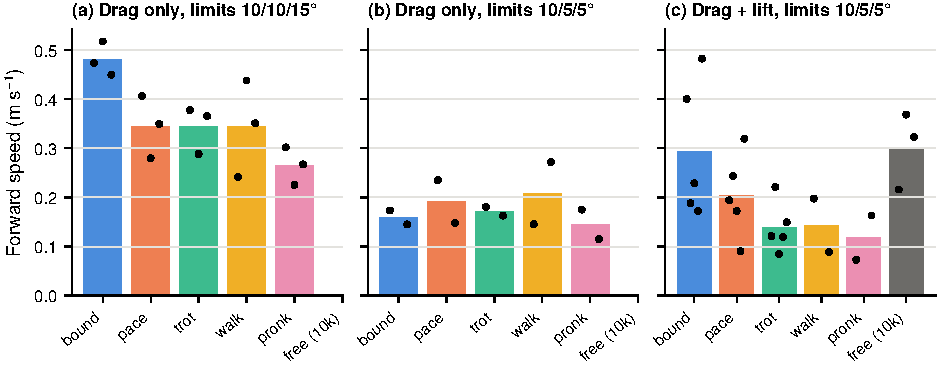
\includegraphics[width=\textwidth]{fig_mj_families}
  \caption[MuJoCo中各步态族的最快步态]{降阶模型中各步态族的最快步态；柱为各种子的均值，点为单个种子的结果。(a)纯阻力，适中限值。(b)纯阻力，严格限值。(c)阻力与升力，严格限值，包括三次$10^4$次评估的自由相位搜索。2500次评估的自由相位搜索未予显示，因为它们尚未收敛。}
  \label{fig:mj-families}
\end{figure}

\section{严格限值下含升力的腿间协调}

在含升力和严格限值的条件下，五个种子上全部十五个对角小跑、同侧步和跳跃步解都是升力推进的、可行的，且不出水（\cref{tab:mj-families}、\cref{fig:mj-families}c）。跳跃步再次最快，其中一个种子达到\SI{0.483}{\metre\per\second}，与适中限值下最快的纯阻力步态一样快，但其舵机几乎始终处于饱和状态。对角小跑的平均功率最低（$1.23\pm\SI{0.90}{\watt}$），但也是三者中最慢的，因此其较低的每米能耗混淆了“经济”与“缓慢”。

为区分二者，在含升力和严格限值的条件下按步态族计算了等速下的最低功率（五个种子，\cref{fig:mj-coord}）。在\SI{0.10}{\metre\per\second}时，对角小跑需要\SI{0.10}{\watt}，而跳跃步需要\SI{0.17}{\watt}；在\SI{0.15}{\metre\per\second}时分别为\SI{0.48}{}和\SI{0.51}{\watt}；各种子的中位数相近。在\SI{0.20}{\metre\per\second}时，对角小跑需要\SI{1.68}{\watt}，而四足齐跳（pronk）和跳跃步分别需要\SI{0.96}{}和\SI{0.98}{\watt}，且五个对角小跑种子中只有三个可行；严格限值下对角小跑的速度极限约为\SI{0.22}{\metre\per\second}。本实验全部55个可行解都是升力推进的。因此，对角协调在低速时至多略为经济；在约\SI{0.15}{\metre\per\second}以上，前后协调既更经济也更快。\Cref{fig:mj-trot}展示了一个速度为\SI{0.221}{\metre\per\second}、功率为\SI{1.03}{\watt}的升力推进对角小跑步态，其舵机从未饱和。

自由相位（free phase）搜索需要更大的评估预算。在2500次评估下，它仅达到\SIrange{0.05}{0.07}{\metre\per\second}；在$10^4$次评估下，三个种子达到$0.303\pm\SI{0.078}{\metre\per\second}$，全部为升力推进，且都收敛到接近跳跃步或四足齐跳的前后协调（偏差为周期的15--19\,\%），而非对角小跑。最佳自由步态以\SI{3.3}{\watt}达到\SI{0.369}{\metre\per\second}，比五个跳跃步最优解中的三个更快，且每米能耗低于全部五个，这表明在固定步态族之外存在更好的协调方式。

\begin{figure}[t]
  \centering
  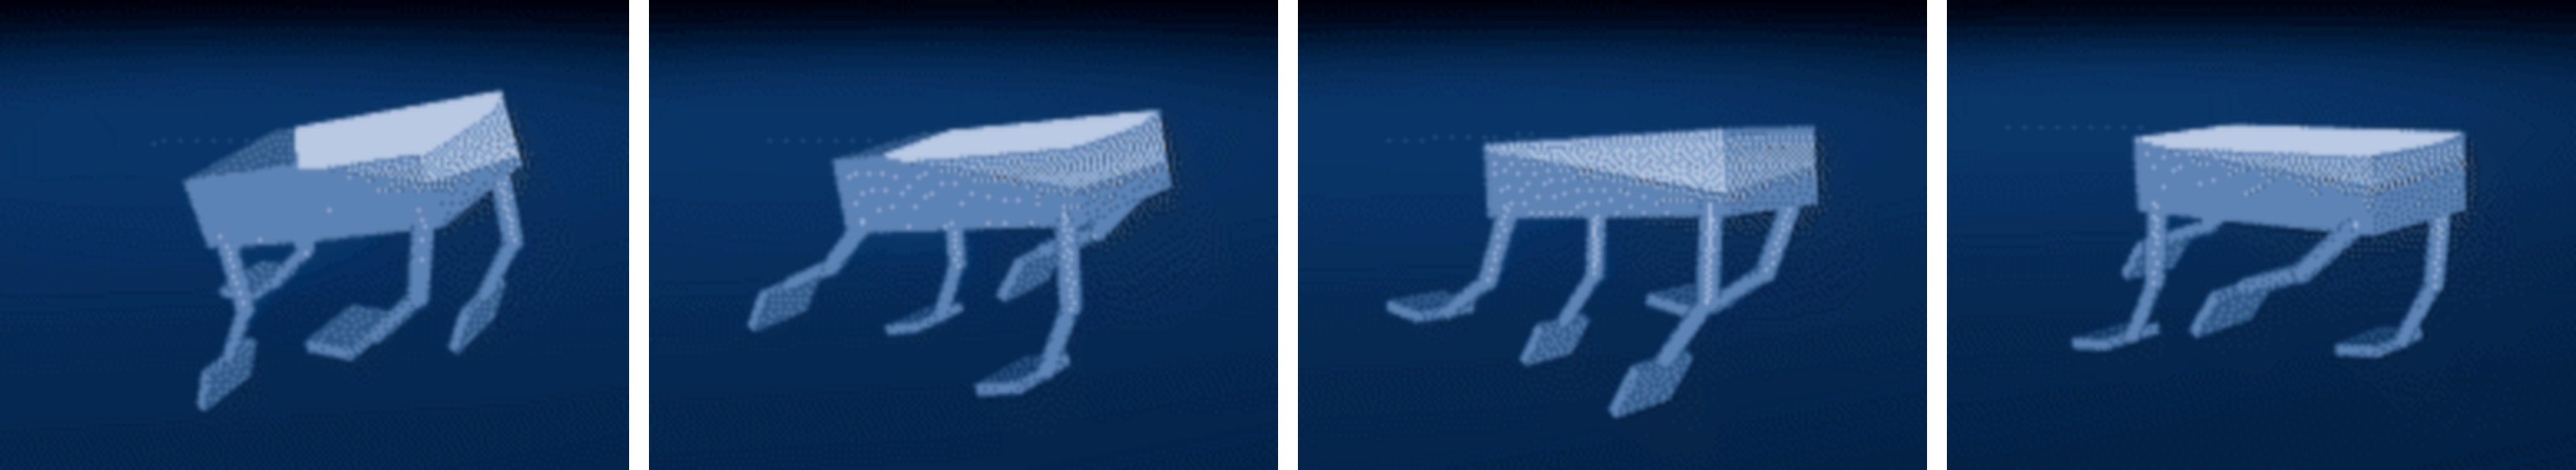
\includegraphics[width=\textwidth]{fig_mj_trot_frames.png}\\[1mm]
  {\small (a)}\\[2mm]
  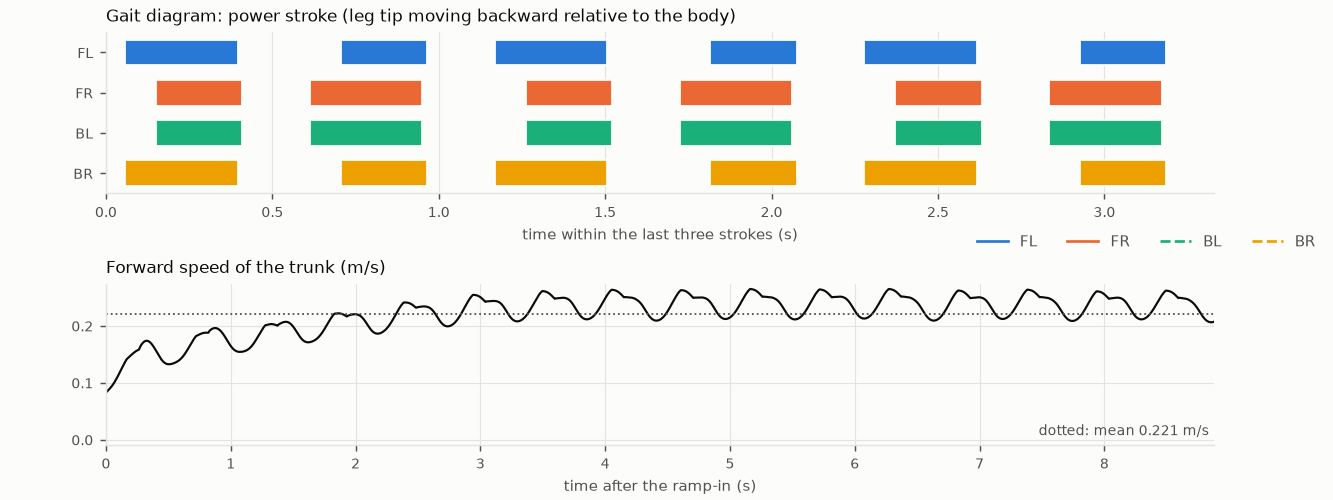
\includegraphics[width=\textwidth]{fig_mj_trot.png}\\
  {\small (b)}
  \caption[MuJoCo中的升力推进对角小跑]{在严格限值下找到的升力推进对角小跑步态（\SI{0.90}{\hertz}，$\mathrm{DUTY}=0.59$，\SI{0.221}{\metre\per\second}，\SI{1.03}{\watt}）。(a) MuJoCo动画中的四帧画面，相邻两帧间隔\SIrange{0.25}{0.30}{\second}，覆盖一个\SI{1.11}{\second}的划动周期；相机跟随躯干。(b) 上图：最后三个周期内四条腿的划水冲程，对角腿同步动作。下图：斜坡引入阶段之后躯干的前进速度，点线为均值。}
  \label{fig:mj-trot}
\end{figure}


\begin{figure}[t]
  \centering
  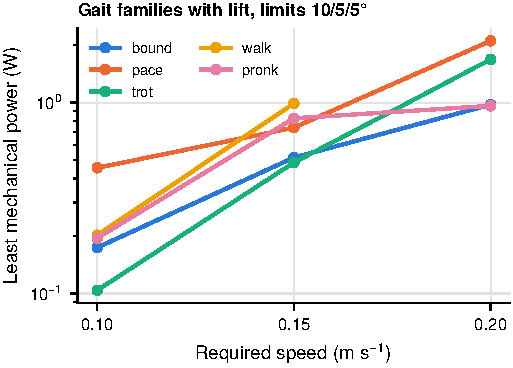
\includegraphics[width=0.58\textwidth]{fig_mj_coord}
  \caption[各步态族的最低功率]{各步态族达到所需速度的最低机械功率，含升力、严格限值（五个种子中的最优值）。}
  \label{fig:mj-coord}
\end{figure}

\section{电功率}

由于大多数最快步态的舵机持续处于力矩限值，基于机械功率的排序可能掩盖了较大的铜损。因此，对全部222个有效最优解重新计算了电功率。按步态族平均，电功率与机械功率的偏差约在$\pm30$\,\%以内，因为在饱和时反电动势项抵消了大部分堵转力矩。例外是适中限值下纯阻力的对角小跑和四足齐跳，其电功率分别高出71\,\%和44\,\%（对角小跑为\SI{19.6}{}而非\SI{11.5}{\watt}）。这使对角小跑在每米能耗上落后于同侧步和行走步；除此之外，本附录的各项结论对电功率同样成立。

\chapter{实时求解器：拖曳仿真与整机趋势}
\label{app:flare-trends}

本附录汇集Flare Live的结果。拖曳仿真（tow run）是\cref{sec:ver-flare}中交叉校核的基础；自航仿真（self-propelled run）反映了整机的趋势，但不能给出可靠的量级。

\section{拖曳仿真}
\label{app:flare}

\begin{table}[H]
  \centering
  \caption[Flare Live拖曳仿真]{采用L0运动的Flare Live拖曳仿真：尾鳍上的流向流体力（尾鳍坐标系）以及整条拍动腿的净推力，单位为\si{\milli\newton}，在$t=\SIrange{3}{9}{\second}$内取平均。}
  \label{tab:app-flare}
  \footnotesize
  \begin{tabular}{@{}lcccccc@{}}
    \toprule
    $\U$ (\si{\metre\per\second}) & 格子 & 尾鳍，拍动 & 尾鳍，不拍动 & 腿净推力 & CFD尾鳍 & $\alpha_{75}$ \\
    \midrule
    0     & \SI{3}{\milli\metre} & 20.0  & --      & 25.7 & 45.5 & \SI{73.8}{\degree} \\
    0.1   & \SI{3}{\milli\metre} & 8.5   & --      & 15.9 & $\approx34$ & \SI{41.1}{\degree} \\
    0.223 & \SI{3}{\milli\metre} & $-0.1$ & $-12.6$ & 9.6  & 21.4 & \SI{19.7}{\degree} \\
    0.223 & \SI{2}{\milli\metre} & 4.1   & $-11.6$ & 5.8  & 21.4 & \SI{19.8}{\degree} \\
    \bottomrule
  \end{tabular}
\end{table}

\section{自航仿真}

鉴于\cref{sec:ver-flare}中的推力亏缺，Flare Live自航仿真仅用于分析趋势（\cref{fig:flare-robot}、\cref{tab:flare}）。取阻力$K=\SI{0.65}{\newton\second\squared\per\metre\squared}$（$D_\text{mid}$），以\SI{2}{\hertz}、目标攻角\SI{18}{\degree}进行对角小跑（trot）时，游速为\SI{0.154}{\metre\per\second}，约为基于CFD预测值的一半，这与所缺失的尾鳍推力相符。
\begin{itemize}
  \item \emph{频率。}在$K=0.65$时，速度随频率按$\U\propto f^{0.71}$增长（$K=3.95$时为$f^{0.51}$），而功率按$f^{1.8}$增长；运输代价（cost of transport）随频率升高。斯特劳哈尔数几乎保持不变。
  \item \emph{攻角。}目标攻角\SI{18}{\degree}给出最高的速度和最低的运输代价；\SI{28}{\degree}略慢，\SI{10}{\degree}则慢得多。控制器确实能保持目标值：在\SI{10}{\degree}的算例中，冲程中段攻角的中位数为\SI{10.1}{\degree}，但尾鳍每个周期需转动\SI{122}{\degree}，且有11\,\%的时间处于限位处。在CFD中，\SI{10}{\degree}规律在该航速下产生的推力最大（\cref{sec:res-lift}）。Flare Live中小攻角所受的惩罚与其未被解析的升力相符；只有“效率在\SIrange{18}{20}{\degree}附近最高”这一结论得到了两种求解器的共同支持。
  \item \emph{阻力。}将$K$由0.65降至0.27（裸船体）仅使速度由\SI{0.154}{}提高到\SI{0.160}{\metre\per\second}，因此在Flare Live中，机器人受限于其推力而非船体。
  \item \emph{姿态。}在对角小跑中，船体的沉浮小于\SI{0.6}{\milli\metre}，俯仰小于\SI{0.3}{\degree}：对角协调使漂浮的机器人保持水平。
\end{itemize}

\begin{table}[t]
  \centering
  \caption[Flare Live自航仿真]{Flare Live自航仿真，对角小跑，$K=\SI{0.65}{\newton\second\squared\per\metre\squared}$。COT $=P_\text{j}/(mg\U)$，其中$P_\text{j}$为关节驱动功率，$m=\SI{0.863}{\kilo\gram}$。}
  \label{tab:flare}
  \small
  \begin{tabular}{@{}lccc@{}}
    \toprule
    算例 & $\U$ (\si{\milli\metre\per\second}) & $P_\text{j}$ (mW) & COT \\
    \midrule
    \SI{2}{\hertz}, $\alpha$ \SI{10}{\degree} & 100.2 & 261 & 0.31 \\
    \SI{2}{\hertz}, $\alpha$ \SI{18}{\degree} & \textbf{153.8} & 239 & \textbf{0.18} \\
    \SI{2}{\hertz}, $\alpha$ \SI{28}{\degree} & 143.8 & 249 & 0.20 \\
    \SI{2.5}{\hertz}, $\alpha$ \SI{18}{\degree} & 183.1 & 355 & 0.23 \\
    \SI{3}{\hertz}, $\alpha$ \SI{18}{\degree} & 205.0 & 488 & 0.28 \\
    \bottomrule
  \end{tabular}
\end{table}

\begin{figure}[t]
  \centering
  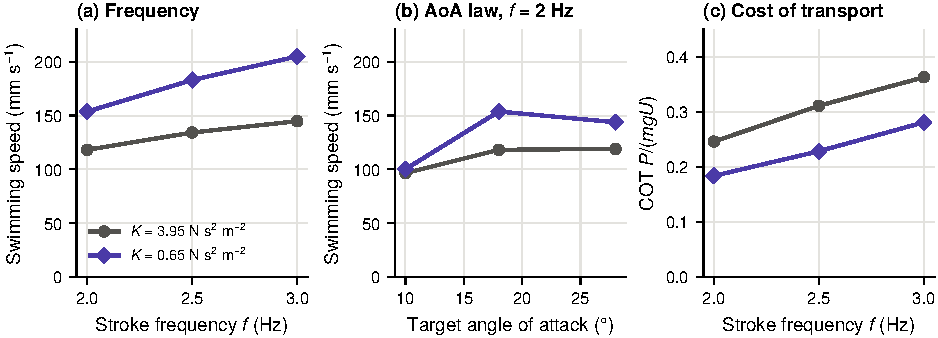
\includegraphics[width=\textwidth]{fig_flare_robot}
  \caption[Flare Live自由游动趋势]{Flare Live中的自航机器人（对角小跑）。(a) 两种船体阻力下速度随划水频率的变化。(b) \SI{2}{\hertz}时速度随目标攻角的变化。(c) 运输代价随频率的变化。}
  \label{fig:flare-robot}
\end{figure}

Flare Live中的关节驱动功率（\SIrange{240}{490}{\milli\watt}）比CFD中的水动力功率（四个尾鳍约\SI{65}{\milli\watt}）高出一个数量级，因为它包含了驱动连杆运动的功率、连杆的惯性以及控制器的控制作用。

\chapter{可复现性}
\label{app:repro}

\section{软件}

\begin{sloppypar}
\begin{itemize}
  \item OpenFOAM v2606，\texttt{overPimpleDyMFoam}；网格由\texttt{blockMesh}和\texttt{snappyHexMesh}生成。算例生成器、运行脚本和后处理均以Python编写（\texttt{make\_leg\_cfd.py}、\texttt{make\_fluke\_cfd.py}、\texttt{fluke\_traj.py}、\texttt{fluke\_forces.py}）。
  \item MuJoCo 3.14及Python包\texttt{cma}；步态优化代码\texttt{swimopt}（\url{https://github.com/lxtuni/swimopt}），其中包括全部234次运行（其中222次有效）的原始结果（\texttt{thesis\_notes/data/all\_runs.csv}）。纯阻力最优解在开启升力后的回放结果（\cref{sec:mj-liftshare}）记录在代码仓库的说明文档中，不在\texttt{all\_runs.csv}内。
  \item Flare Live及脚本\texttt{run\_float.py}（自航仿真，self-propelled run）和\texttt{bench\_foil.py}（拖曳仿真，tow run）。
\end{itemize}
\end{sloppypar}
\TODO{补充CFD与Flare Live脚本的代码仓库以及最终版本的提交哈希值。}

\section{MuJoCo设置}

\begin{table}[H]
  \centering
  \caption[MuJoCo设置]{基于降阶模型的步态优化（reduced-order gait optimization）的设置。}
  \label{tab:app-mujoco}
  \small
  \begin{tabularx}{\textwidth}{@{}l>{\raggedright\arraybackslash}X@{}}
    \toprule
    项目 & 取值 \\
    \midrule
    时间步长，积分器 & \SI{2}{\milli\second}，implicit-fast \\
    评估 & 稳定\SI{1.0}{\second}，渐入\SI{1.5}{\second}，计分\SI{8}{\second}并向上取整为整数个周期 \\
    舵机 & 位置舵机，刚度60，临界阻尼，$\tau_s=\SI{3}{\newton\metre}$，$\omega_\text{max}=\SI{400}{\degree\per\second}$ \\
    脚蹼系数 & $C_D=(2.2,0.10,0.10)$，$C_a=1.0$，$c_v=0.05$，$c_l=1.1$ \\
    杆件系数 & $C_D=(0.5,0.5,0.25)$，$C_a=0.3$，$c_v=0.02$ \\
    躯干系数 & $C_D=(0.9,1.6,1.8)$，$C_a=0.2$，$c_v=0.10$ \\
    步态 & $H=2$；$f\in[0.2,2.5]$\,Hz；DUTY $\in[0.25,0.75]$；$A\in[0,0.9]$\,rad；$q_0\in[-0.5,0.5]$\,rad \\
    CMA-ES & 种群规模16，$\sigma_0=0.25$，2500次评估（自由相位为$10^4$次），非零种子 \\
    限值 & 航向/横滚/俯仰RMS $10/10/\SI{15}{\degree}$或$10/5/\SI{5}{\degree}$；注明之处另要求出水比例$\le5$\,\%；\cref{sec:mj-liftshare}中的阻力型划动另加升力推力占比$s_L\le0.1$ \\
    \bottomrule
  \end{tabularx}
\end{table}

\section{发现并修正的模型错误}

工作过程中发现了仿真设置中的若干错误，并在生成本文所报告的结果之前予以修正。之所以列出这些错误，是因为它们很容易重犯。
\begin{itemize}
  \item MJCF默认以度为单位读取关节范围；本意以弧度表示的$\pm1.3$范围将每个关节都锁定在了$\pm\SI{1.3}{\degree}$。此次修正之前的所有结果均已舍弃。
  \item 在运行时更改刚体质量而未重新计算MuJoCo的派生常量，导致附加质量对单个自由刚体失效，并在一项动量守恒测试中造成36\,\%的误差。
  \item 从URDF导入的视觉几何体和碰撞几何体都被施加了水动力，使浮力、阻力和附加质量加倍。
  \item 一旦腿部可以自由运动，对速度和姿态的加性加权便会产生强烈横滚和偏航的最优解；它已被式\eqref{eq:feasibility}的可行性优先（feasibility-first）表述所取代。
  \item 升力占比最初定义为$|I_L|/(|I_L|+|I_\text{drag}|)$。由于稳态游动时升力冲量与阻力冲量相互抵消，该值对任何含升力的步态都约为0.5；将其用作限值时，只有几乎不动的步态才能满足。该指标已被式\eqref{eq:liftshare}中的$s_L$取代，使用旧指标的运行均已作废。
  \item 在尾鳍CFD中，一个未在尾鳍周围加密的粗背景网格（background mesh）导致了挖洞（hole cutting）失败，几乎整个背景网格都被移除；现在会自动检查洞单元的数量。
\end{itemize}


\printbibliography[heading=bibintoc,title={参考文献}]
\end{document}
